\documentclass[a4paper, 12pt]{article}
\usepackage[utf8]{inputenc}
\usepackage[T1, T2A]{fontenc}
\usepackage[a4paper, top=2cm, bottom=2cm, left=1cm, right=1cm, marginparwidth=1.75cm]{geometry}
\usepackage{graphicx}
\usepackage{amsmath}
\usepackage{amssymb}
\usepackage{amsfonts}
\usepackage{indentfirst}
\usepackage[english, russian]{babel}
\usepackage[section,above,below]{placeins}
\usepackage{pdfpages} 
\usepackage{svg}

\newcommand{\V}[1]{\int_Q #1(y) E(x-y) dy}
\newcommand{\R}[1]{\mathbb{R}^#1}
\newcommand{\ro}{ \tilde \rho_N}
\newcommand{\der}[2]{\dfrac{\partial #1}{\partial #2}}

\begin{document}
  
\subsubsection{Кратное интегрирование по областям с параметризуемой границей}
Пусть $Q$ -- область, по которой ведётся интегрирование, причём она имеет параметризуемую границу; $f$ -- функция под интегралом. Область можно разбить на сетку, например, следующим классическим способом (Рис. \ref{classic}, для простоты $Q$ --- круг).

\begin{figure}[h!]
  \noindent\centering{
  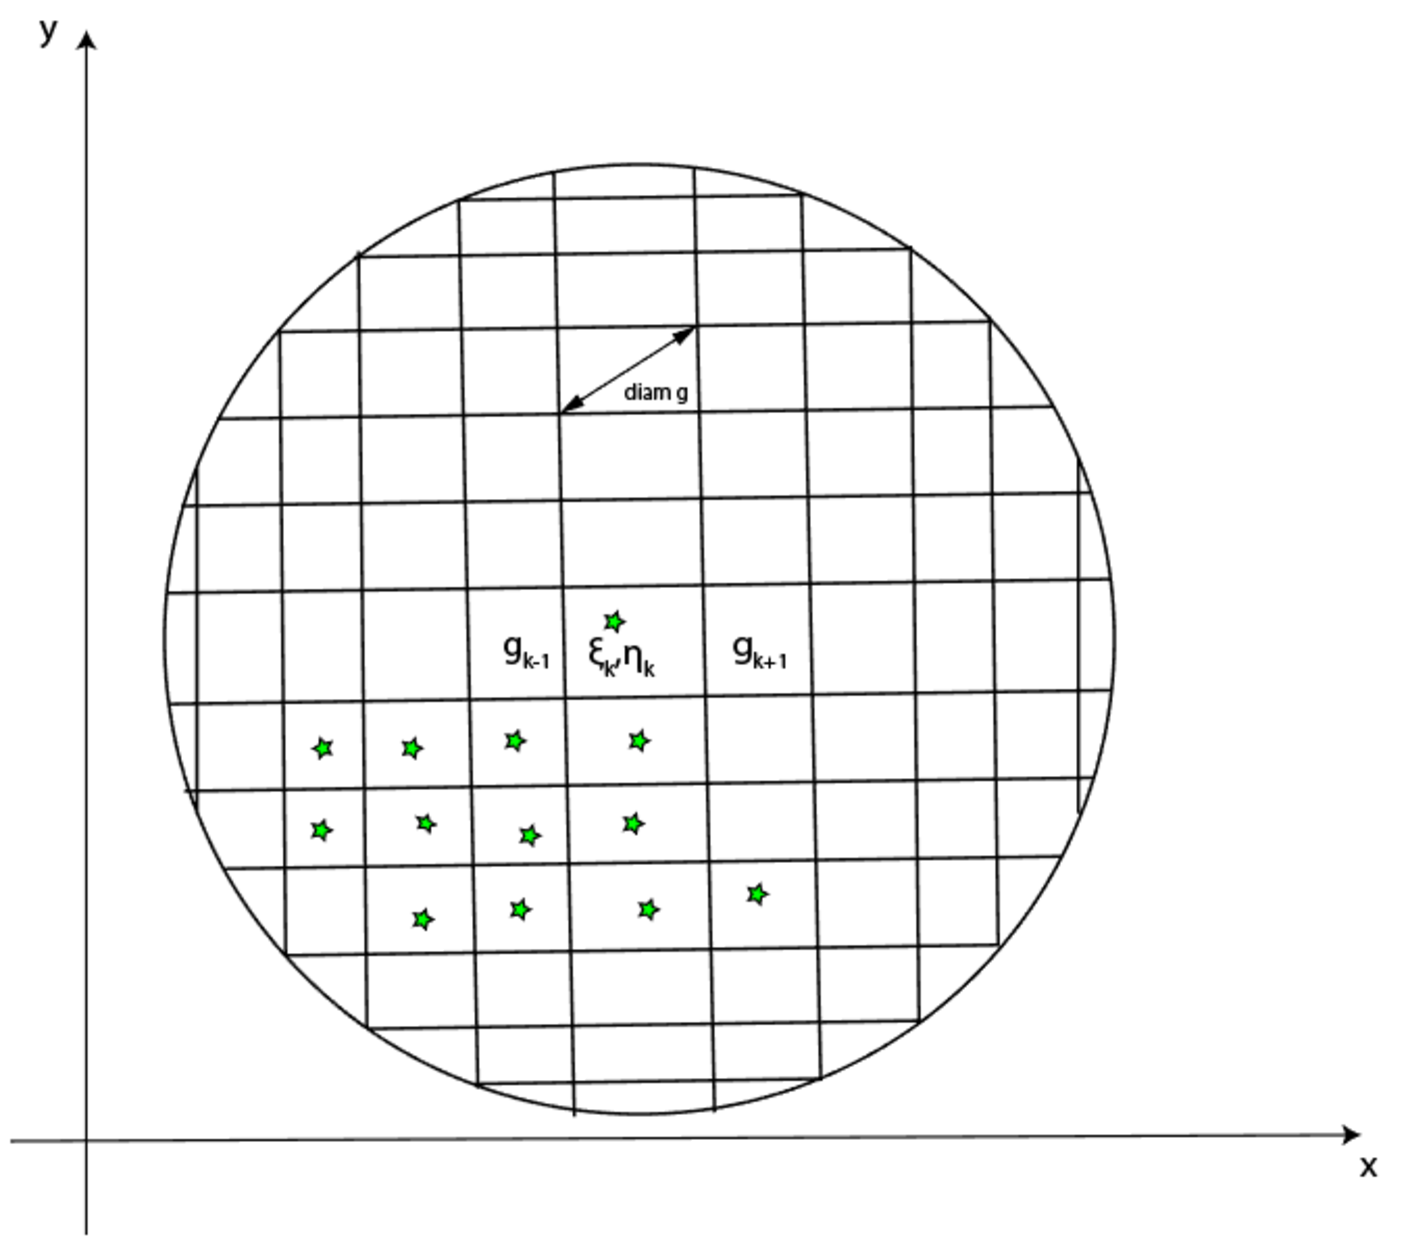
\includegraphics[width=14cm]{4.pdf}
}
  \caption{Разбиение области на сетку классическим способом}
  \label{classic}
  \end{figure} 

В таком случае по определению кратного интеграла $$\int_Q f(x,y)dx dy=\lim_{\text{diam} g_k \rightarrow 0} \sum_k S(g_k) f(\xi_k,\eta_k),$$ где $g_k$ -- обозначение $k$-й ячейки ($Q = \bigcup_k g_k$), $\text{diam} g_k$ -- её диаметр, $S(g_k)$ -- площадь, $f(\xi_k,\eta_k)$ -- значение $f$ в любой точке внутри ячейки.
Указанное равенство справедливо независимо от того, как именно область $Q$ разбивается на ячейки, поэтому, имея задание границы области в виде ${\bf r}={\bf r}(t,r), t \in [t_0, t_{\max}]$, область легко можно разбить на $k$ вложенных друг в друга колец\footnote{В многомерном случае правильнее будет называть их слоями.}, ограниченных кривыми ${\bf r}(t,r_i),{\bf r}(t,r_{i+1}),i =1,\dots,k$, а каждое кольцо разбить на ячейки в соответствии с изменением параметра $t$ (Рис.\ref{plast}).

\begin{figure}[h!]
  \noindent\centering{
  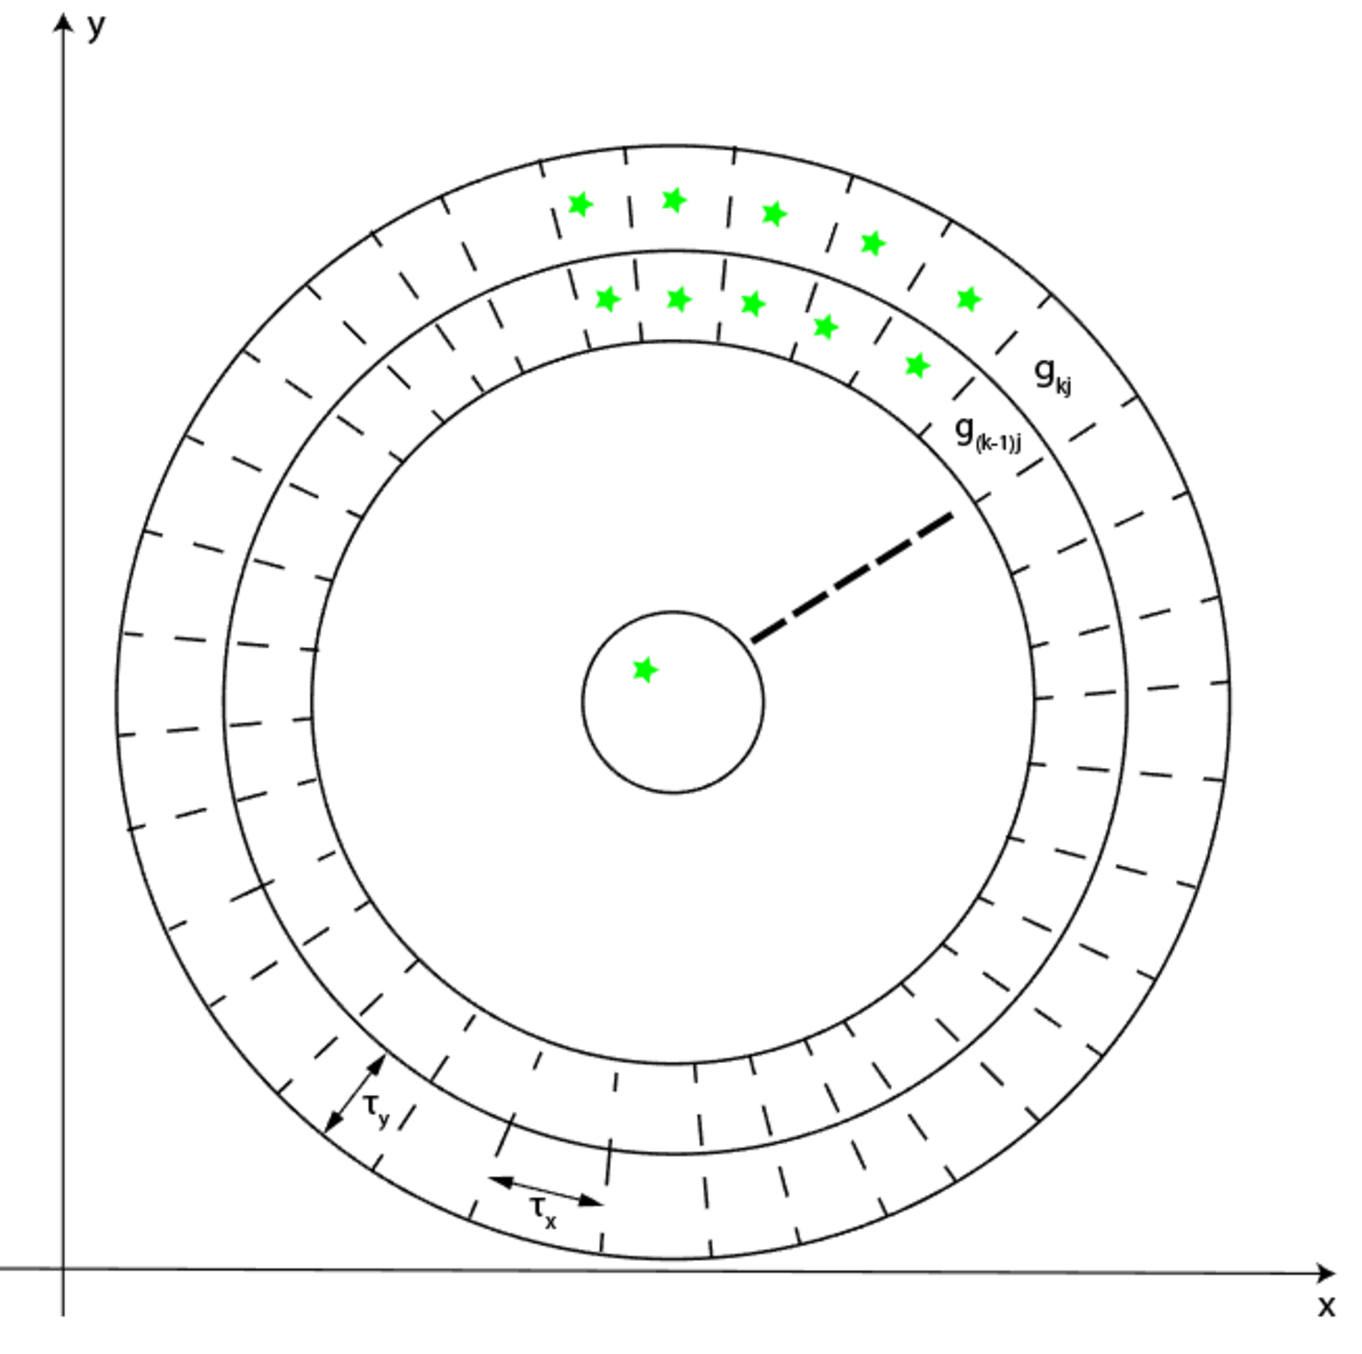
\includegraphics[width=14cm]{5.pdf}
}
  \caption{Разбиение области на сетку в соответствии с параметризацией границы}
  \label{plast}
  \end{figure} 

Тогда $$\int_Q f(x,y)dx dy=\lim_{\tau_x, \tau_y \rightarrow 0} \sum_k \sum_j S(g_{kj}) f({\bf r}(t_{j+\frac{1}{2}\tau_x},r_{k+\frac{1}{2}\tau_y})),$$
где $\tau_y$ --- "радиус"\ колец (соответственно шаг по радиусу области, определяющий количество колец),
$\tau_x$ --- шаг "по кольцу" (по параметру $t$), $S(g_{kj})$ -- площадь ячейки $j$ из $k$-го кольца,
$f({\bf r}(t_{j+\frac{1}{2}\tau_x},r_{k+\frac{1}{2}\tau_y}))$ --- значение функции в точке примерно в середине ячейки $j\ k$-го кольца. 
Сразу отметим, что не обязательно брать одни и те же параметры $\tau_x, \tau_y$ для всех колец, вдобавок ясно, что $S(g_{kj}) \rightarrow \tau_x \tau_y, \tau_x, \tau_y \rightarrow 0$.

Таким образом, получено разбиение области $Q$ на кольца, которое удобно выполнить, зная задание границы $Q$ в виде ${\bf r}=(t,r), t \in [t_0,t_{\max}]$. Тогда интеграл по $Q$ приближённо равен сумме интегралов по всем кольцам, причём приближённо, потому что в центре области остаётся вырожденное кольцо, интеграл по которому будем считать неизвестным; вместо интеграла по вырожденному кольцу можно взять произведение площади этого кольца и точки в центре, если известна площадь; ясно, что при уменьшении радиуса $\tau_y$ кольца вклад интеграла по вырожденному кольцу будет уменьшаться.
Следовательно, задача интегрирования по области свелась к задаче интегрирования по кольцу.

Разобьём кольцо на $n$ секторов, как показано на Рис. \ref{plast2}.
\begin{figure}[h!]
  \noindent\centering{
  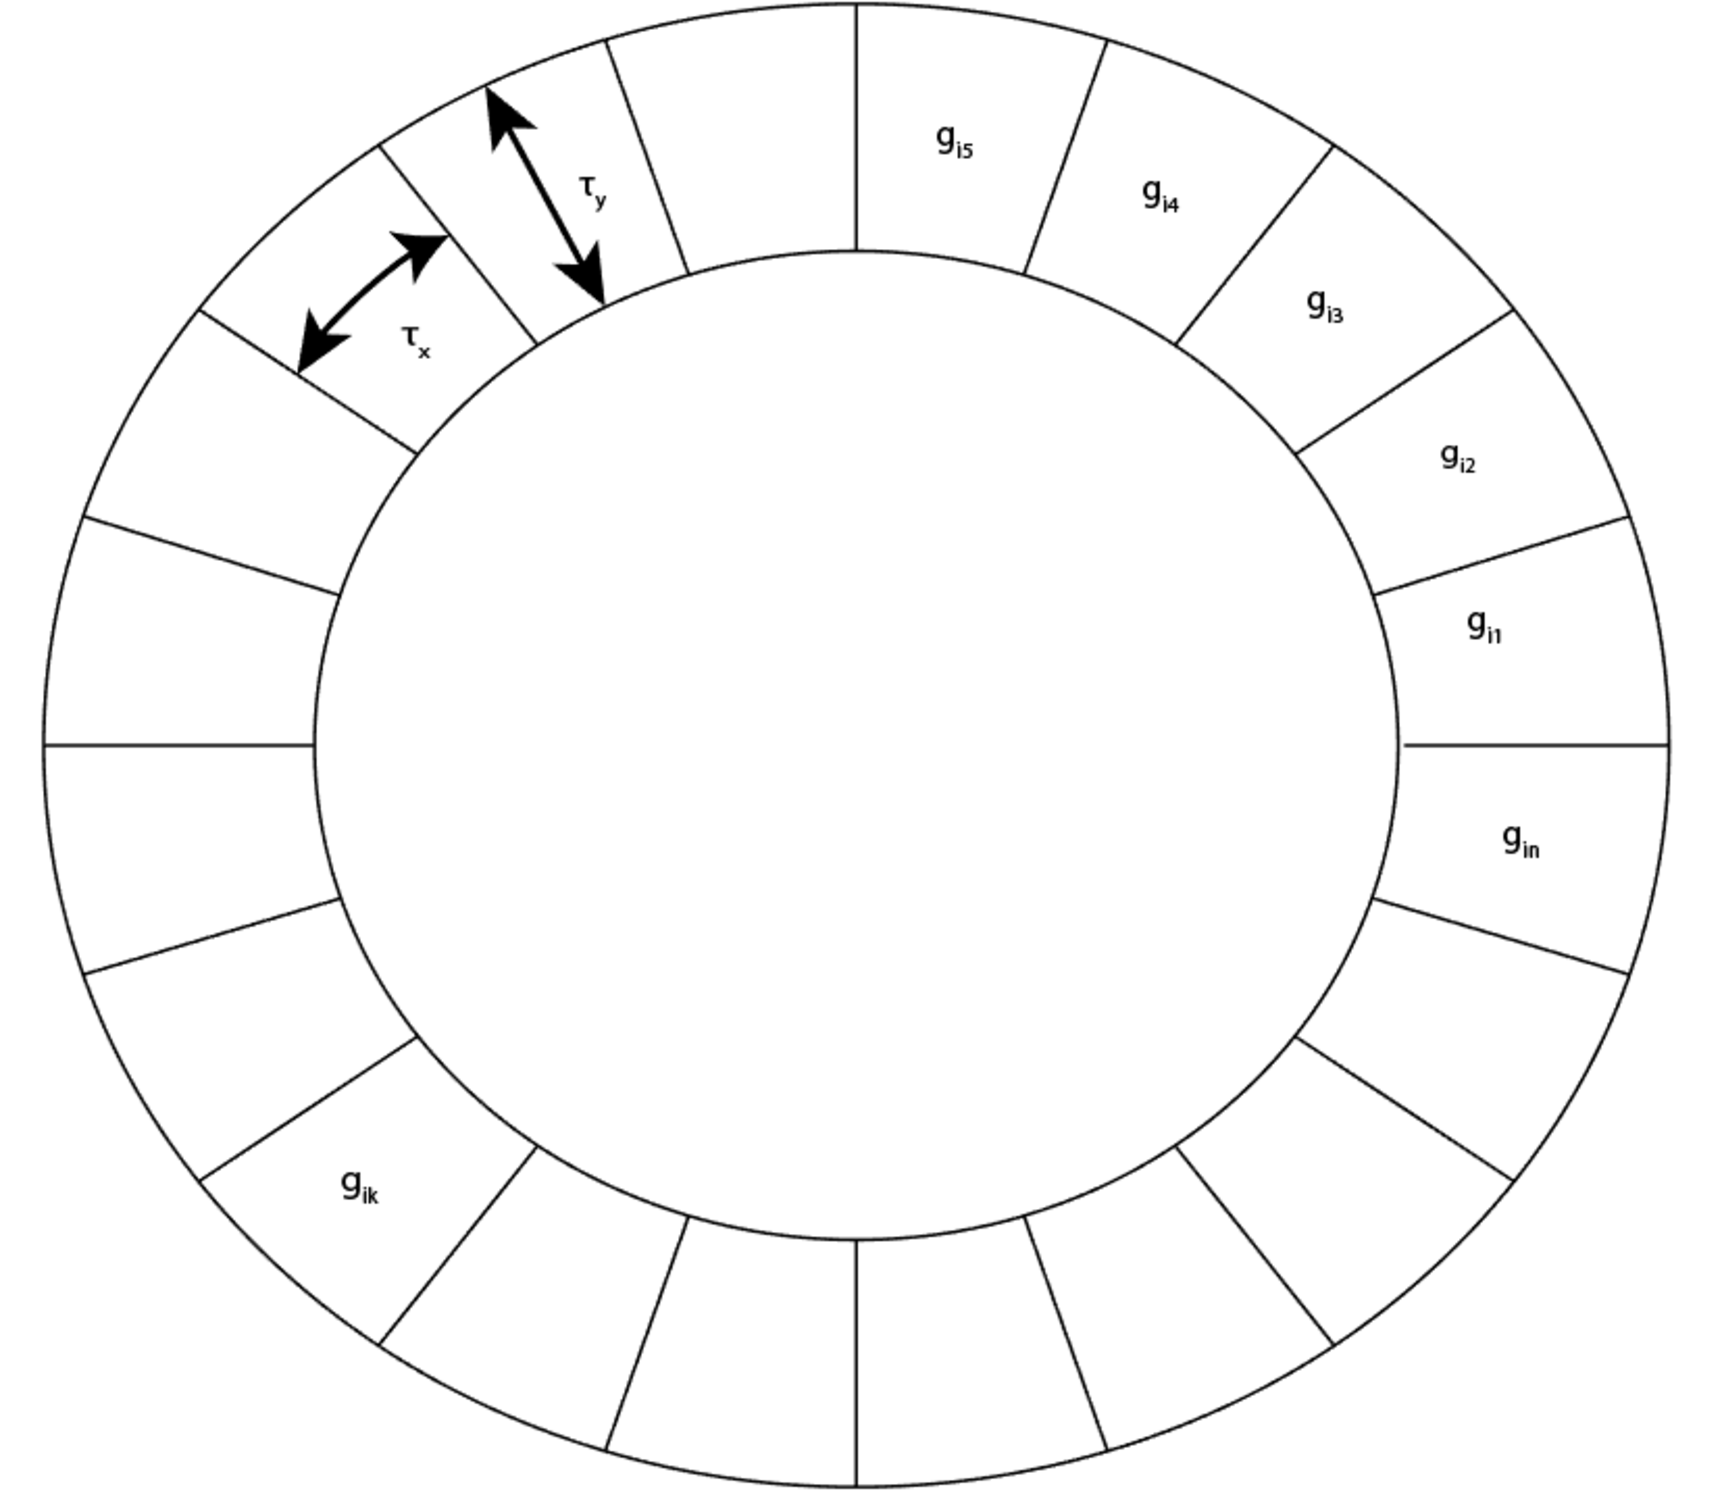
\includegraphics[width=12cm]{6.pdf}
}
  \caption{Разбиение кольца на сетку в соответствии с параметризацией границы}
  \label{plast2}
  \end{figure} 
Отрезки, разделяющие секторы, имеют концы ${\bf r}(t_j,r_i), {\bf r}(t_j,r_{i+1}), i= 1, \dots, k, j=1,\dots,n, t_j=t_0+\tau_x j, r_i =\tau_y i$. Очевидно, что при $\tau_x, \tau_y \rightarrow 0$ площадь каждого сектора стремится к $\tau_x \tau_y$ (независимо от формы кривой), а интеграл от функции $f$ по этому сектору -- к $\tau_x \tau_y f(t_j+\frac{1}{2}\tau_x ,r_i + \frac{1}{2} \tau_y)=\tau_x \tau_y f(t_0+(j+\frac{1}{2})\tau_x ,(i+\frac{1}{2}) \tau_y)$, если, конечно, $f$ не имеет особенностей в центре сектора.
Запишем полученную формулу в виде:
$$\int_{g_{ij}}f(x,y)dx dy \approx \tau_x \tau_y f \left(t_0+\left(j+\frac{1}{2}\right)\tau_x ,\left(i+\frac{1}{2}\right) \tau_y\right)=\frac{\tau_x \tau_y}{\tau_y} \tau_y f \left(t_0+\left(j+\frac{1}{2}\right)\tau_x ,\left(i+\frac{1}{2}\right) \tau_y\right).$$
Просуммировав по всем секторам $g_{ij}$, получим интеграл по кольцу $g_{i}$:
$$\sum_j \frac{\tau_x \tau_y}{\tau_y} \tau_y f \left(t_0+\left(j+\frac{1}{2}\right)\tau_x ,\left(i+\frac{1}{2}\right) \tau_y\right) \approx \int_{g_i} f(x,y) dx dy,$$
который есть ничто иное как:
$$\int_{g_i} f(x,y)dx dy=\frac{S(g_i)}{t_{\max}-t_0} \int^{t_{\max}}_{t_0} f\left({\bf r}\left(t,\left(i+\frac{1}{2}\right)\tau_y\right)\right)dt=\frac{S(g_i)}{l} \int_l f(x,y) dl,$$
то есть интеграл по кольцу может быть выражен через произведение площади кольца и криволинейного интеграла по подобной границам кривой, проходящей по середине кольца (Рис. \ref{plast3}).
\begin{figure}[h!]
  \noindent\centering{
  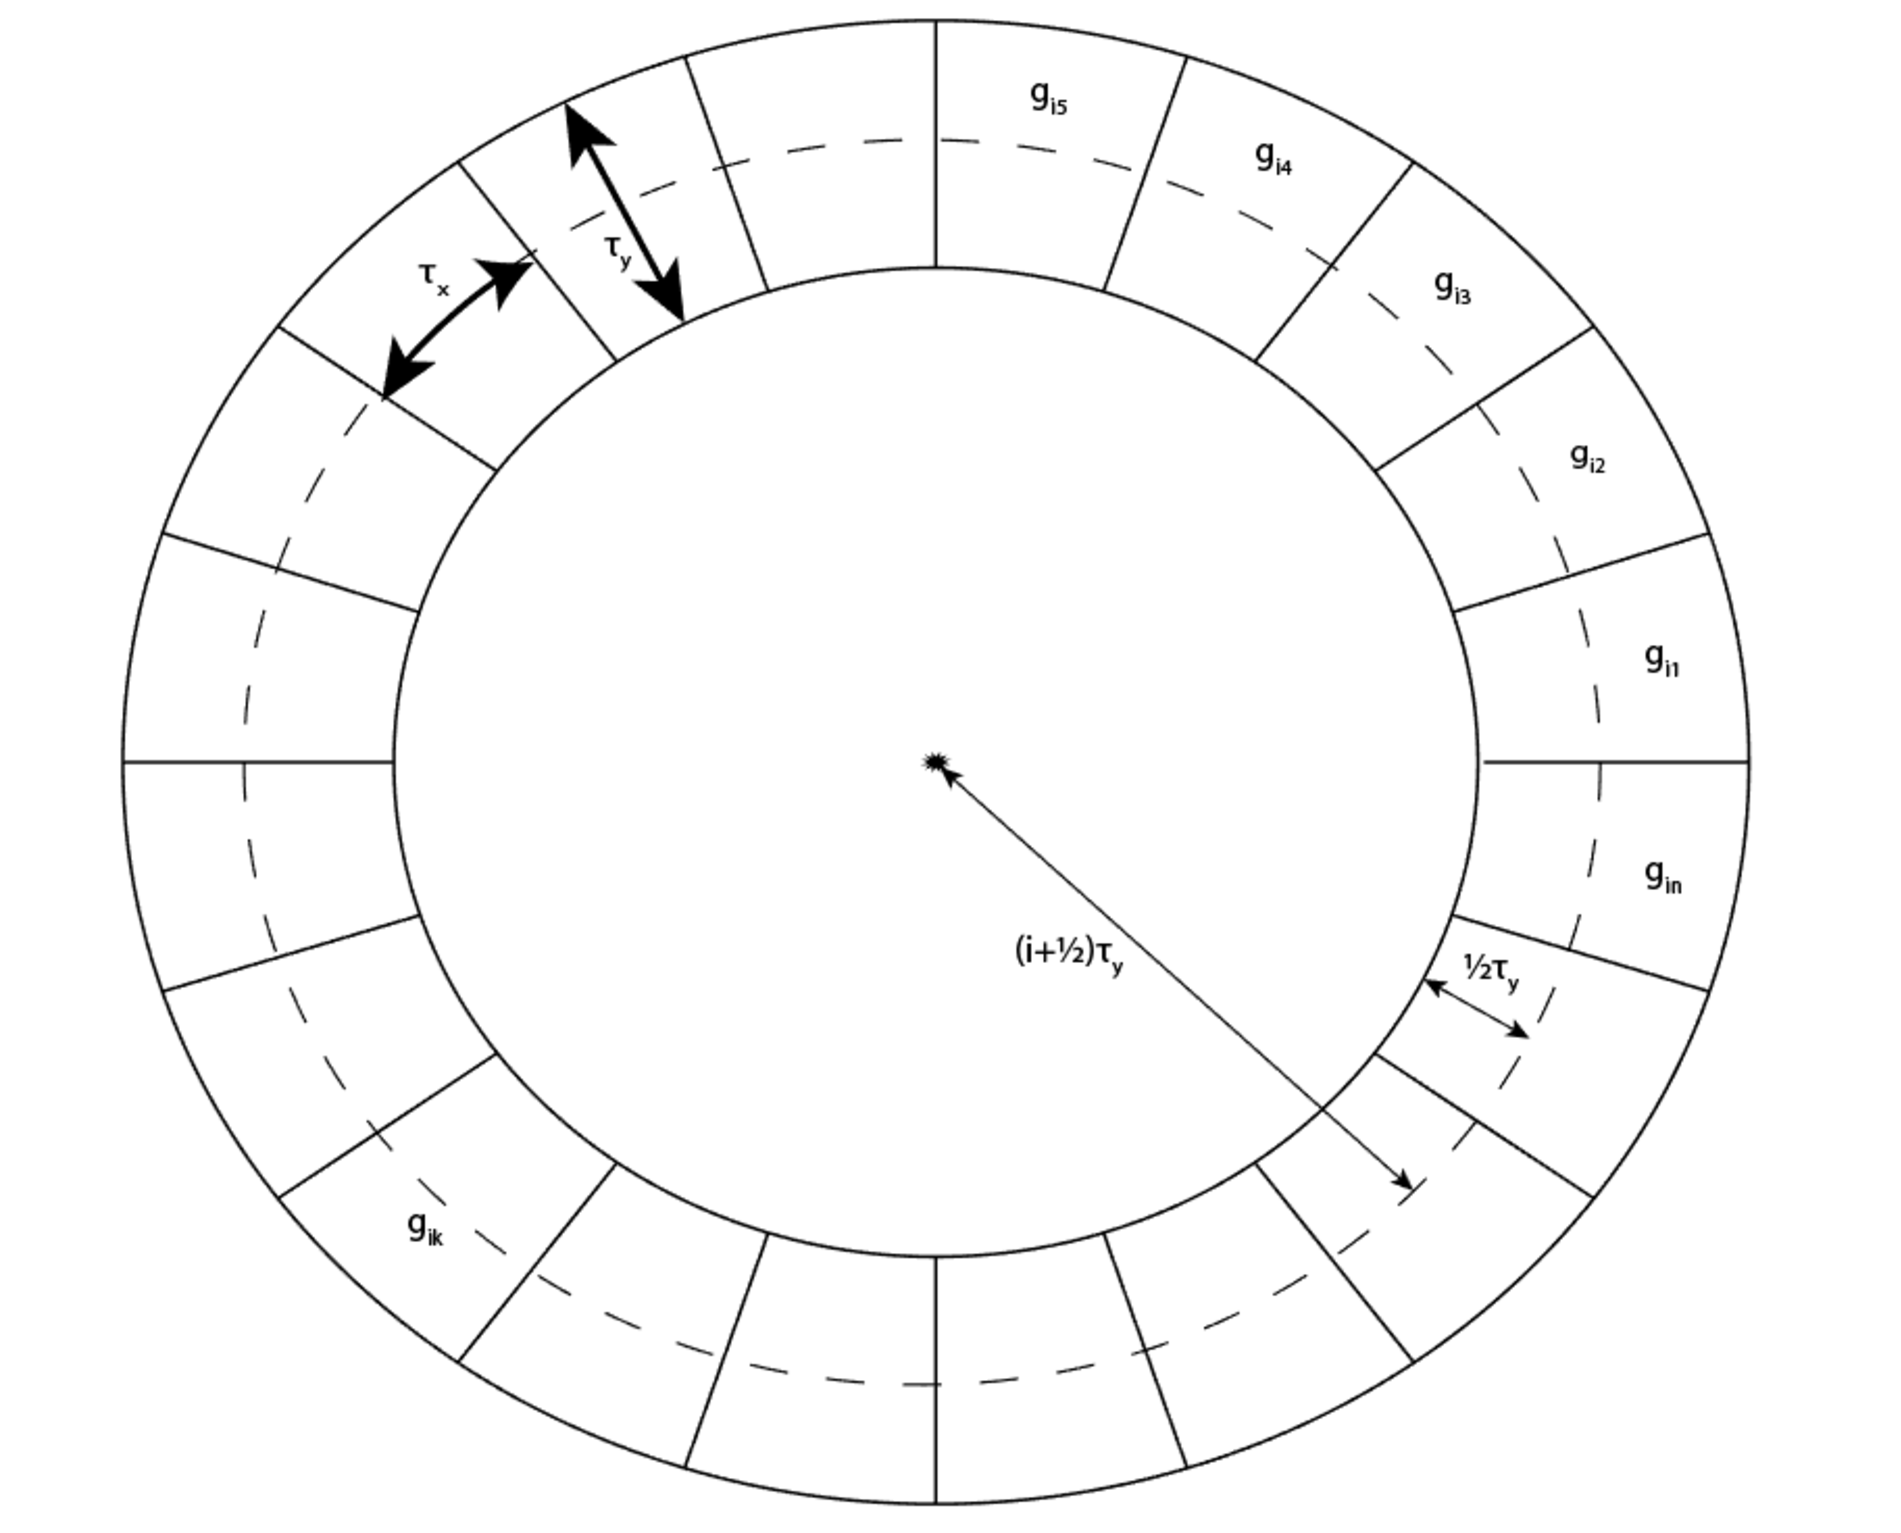
\includegraphics[width=12cm]{7.pdf}
}
  \caption{Кривая посередине кольца, по которой вычисляется криволинейный интеграл}
  \label{plast3}
  \end{figure} 

Таким образом, получено выражение кратного интеграла через сумму определённых:
$$\int_Q f(x,y)dx dy \approx \sum_i \frac{S_i}{t_{\max}-t_0} \int^{t_{\max}}_{t_0} f\left({\bf r}\left(t,\left(i+\frac{1}{2}\right)\tau_y\right)\right)dt.$$  

{\bf Замечания}:
\begin{enumerate}
  \item На самом деле при интегрировании можно брать любой контур внутри кольца, но при специальном задании границ кольца в виде ${\bf r}(t,r)$ (на что рассчитывает метод) удобнее брать именно подобную кривую.
   \item Если нет возможности выразить функцию площади кольца $S_i=S(\tau_y,(i+0.5)\tau_y)$, в качестве площади при достаточно малых $\tau_y$ можно взять $S_i=\pi ((i+1)\tau_y)^2-\pi (i \tau_y)^2= \pi \tau^2_y (2i+1)$
   \item Как правило, при параметризации $t_0=0$, но $t_{\max}$ зависит от радиуса кривой $r=(i+0.5)\tau_y$, поэтому $\frac{1}{t_{\max}-t_0}$ не всегда является константным выражением и может быть вынесено за знак суммирования.
\item Для возможности равномерного интегрирования указанных криволинейных интегралов следует использовать естественную параметризацию.
\item Для круговой области вычислять кратный интеграл можно и классическими способами, однако если область имеет более сложную форму, классические методы будет чрезвычайно тяжело использовать. 
\end{enumerate}

{\bf Тесты.} На следующих рисунках (рисунки \ref{circ5}-\ref{hcirc2}) показаны результаты использования описанного метода интегрирования для разных областей и разных подинтегральных функций.
Области и функции взяты простыми, так как для сложных областей и функций трудно  аналитически найти интеграл, с которым требуется провести сравнение.
Замечено два типа поведения погрешности в зависимости от числа колец в интеграле: логарифмическое убывание и малое приближённо константное значение (на самом деле очень медленное логарифмическое убывание); при этом произведение {\it погрешность интегрирования} $\cdot$ {\it время вычислений} в первом случае логарифмически убывает, во втором --- логарифмически растёт.
Требуется также отметить, что графики рисовались в логарифмической шкале, поэтому точки с погрешностью не больше машинного нуля либо временем вычисления меньше машинного минимума --- не изображались. 

\begin{figure}[h!]
    \noindent\centering{
    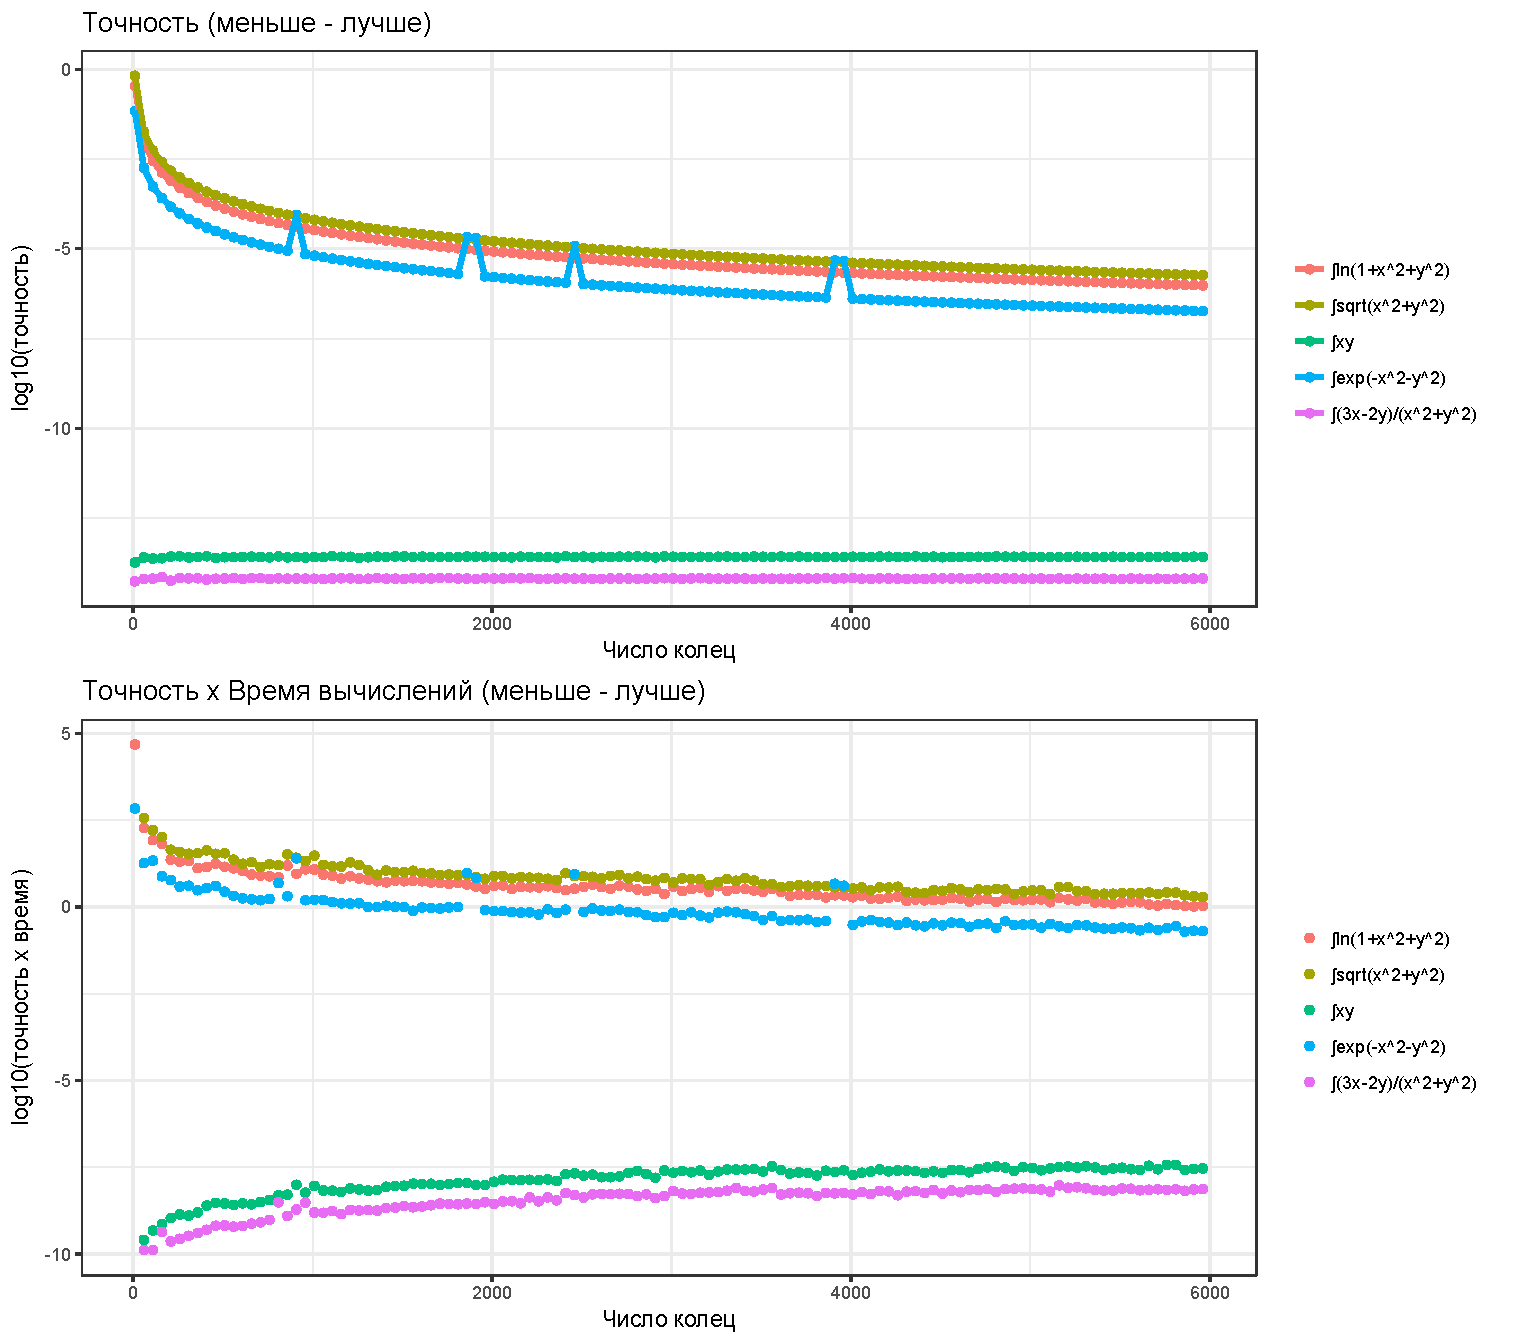
\includegraphics[width=\linewidth]{circ5.pdf}
  }
    \caption{Точность и отношение точность-время от интегрирования для круга радиуса $r=5$}
    \label{circ5}
    \end{figure} 
  
    \begin{figure}[h!]
      \noindent\centering{
      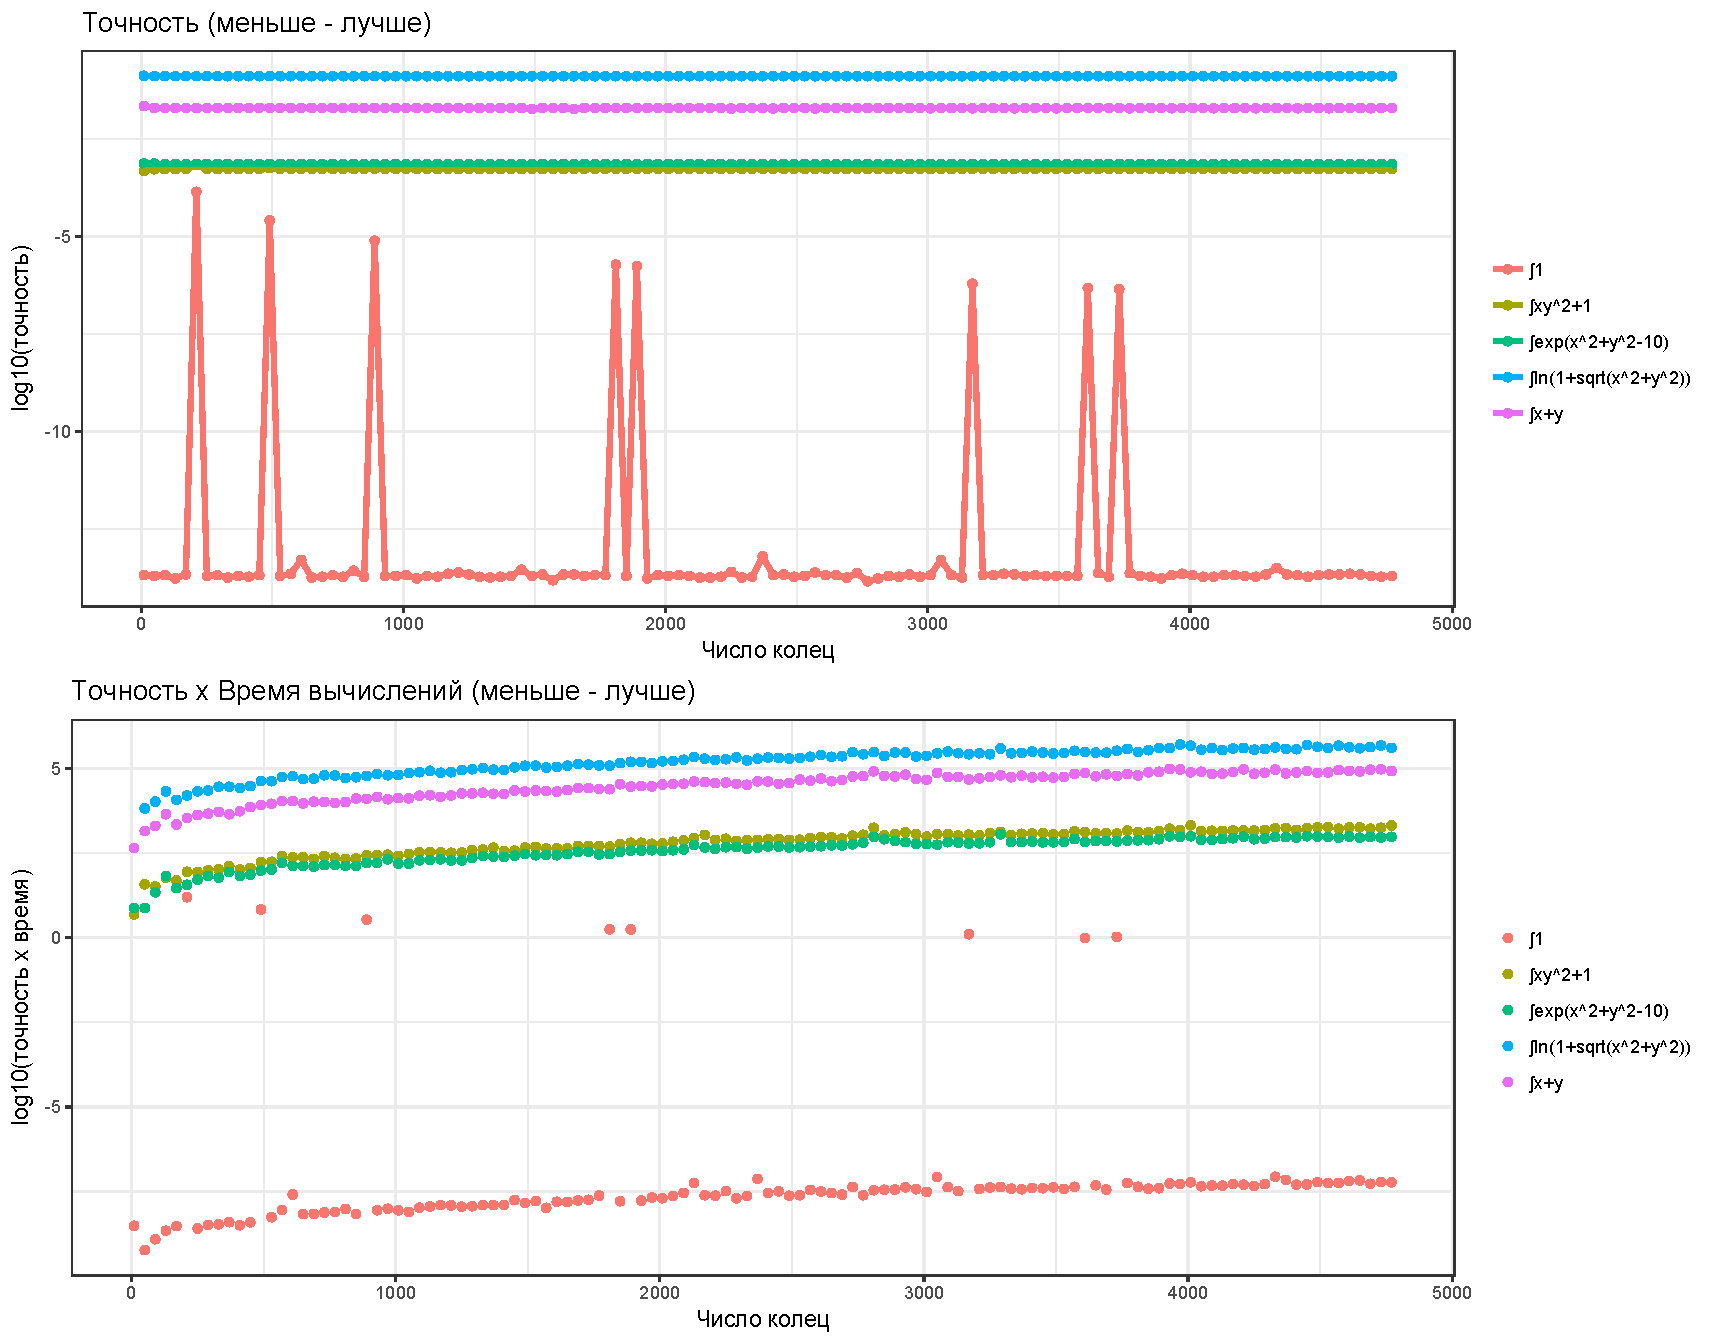
\includegraphics[width=\linewidth]{hcirc.pdf}
    }
      \caption{Точность и отношение точность-время от интегрирования для верхнего полукруга радиуса $r=2$}
      \label{hcirc2}
      \end{figure} 

      \begin{figure}[h] 
        \center{\begin{minipage}[h]{\linewidth} 
        \center{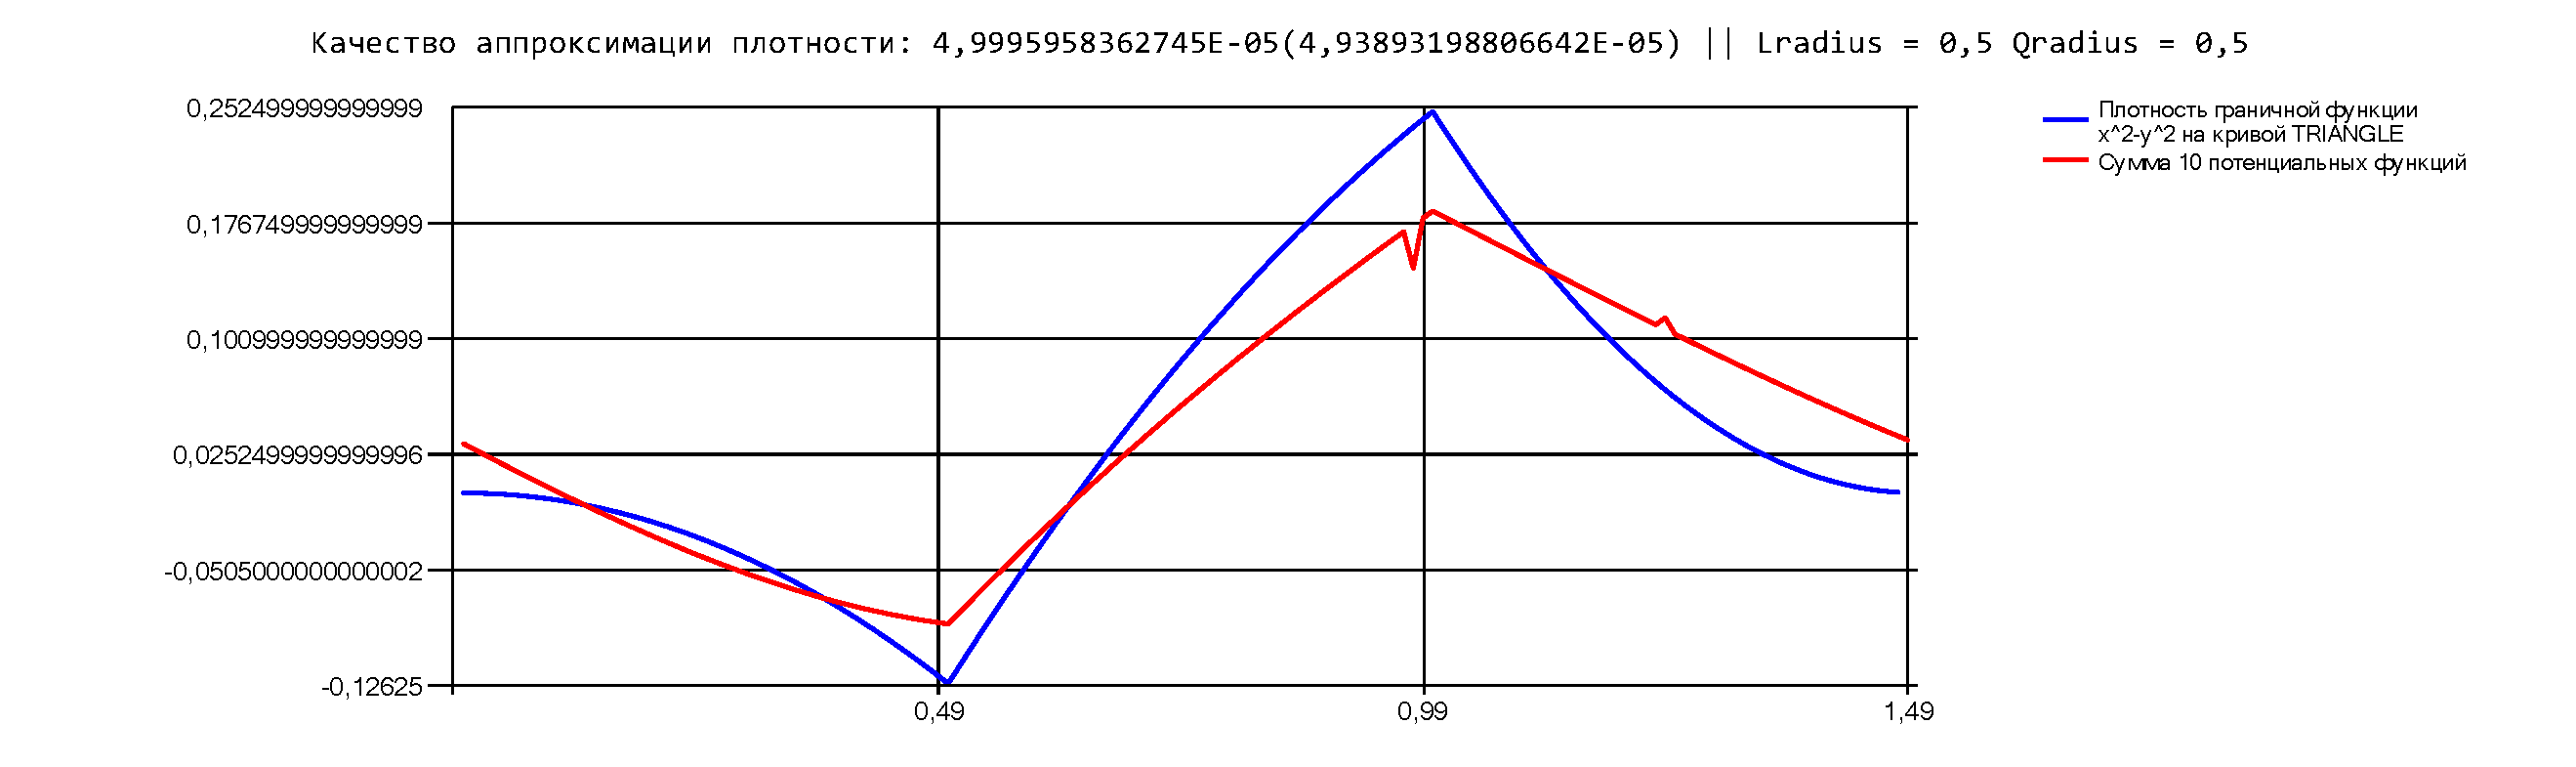
\includegraphics[width=0.8\linewidth]{d11.pdf} \\ для плотности} 
        \end{minipage}} 
        \vfill 
        \center{\begin{minipage}[h]{\linewidth} 
        \center{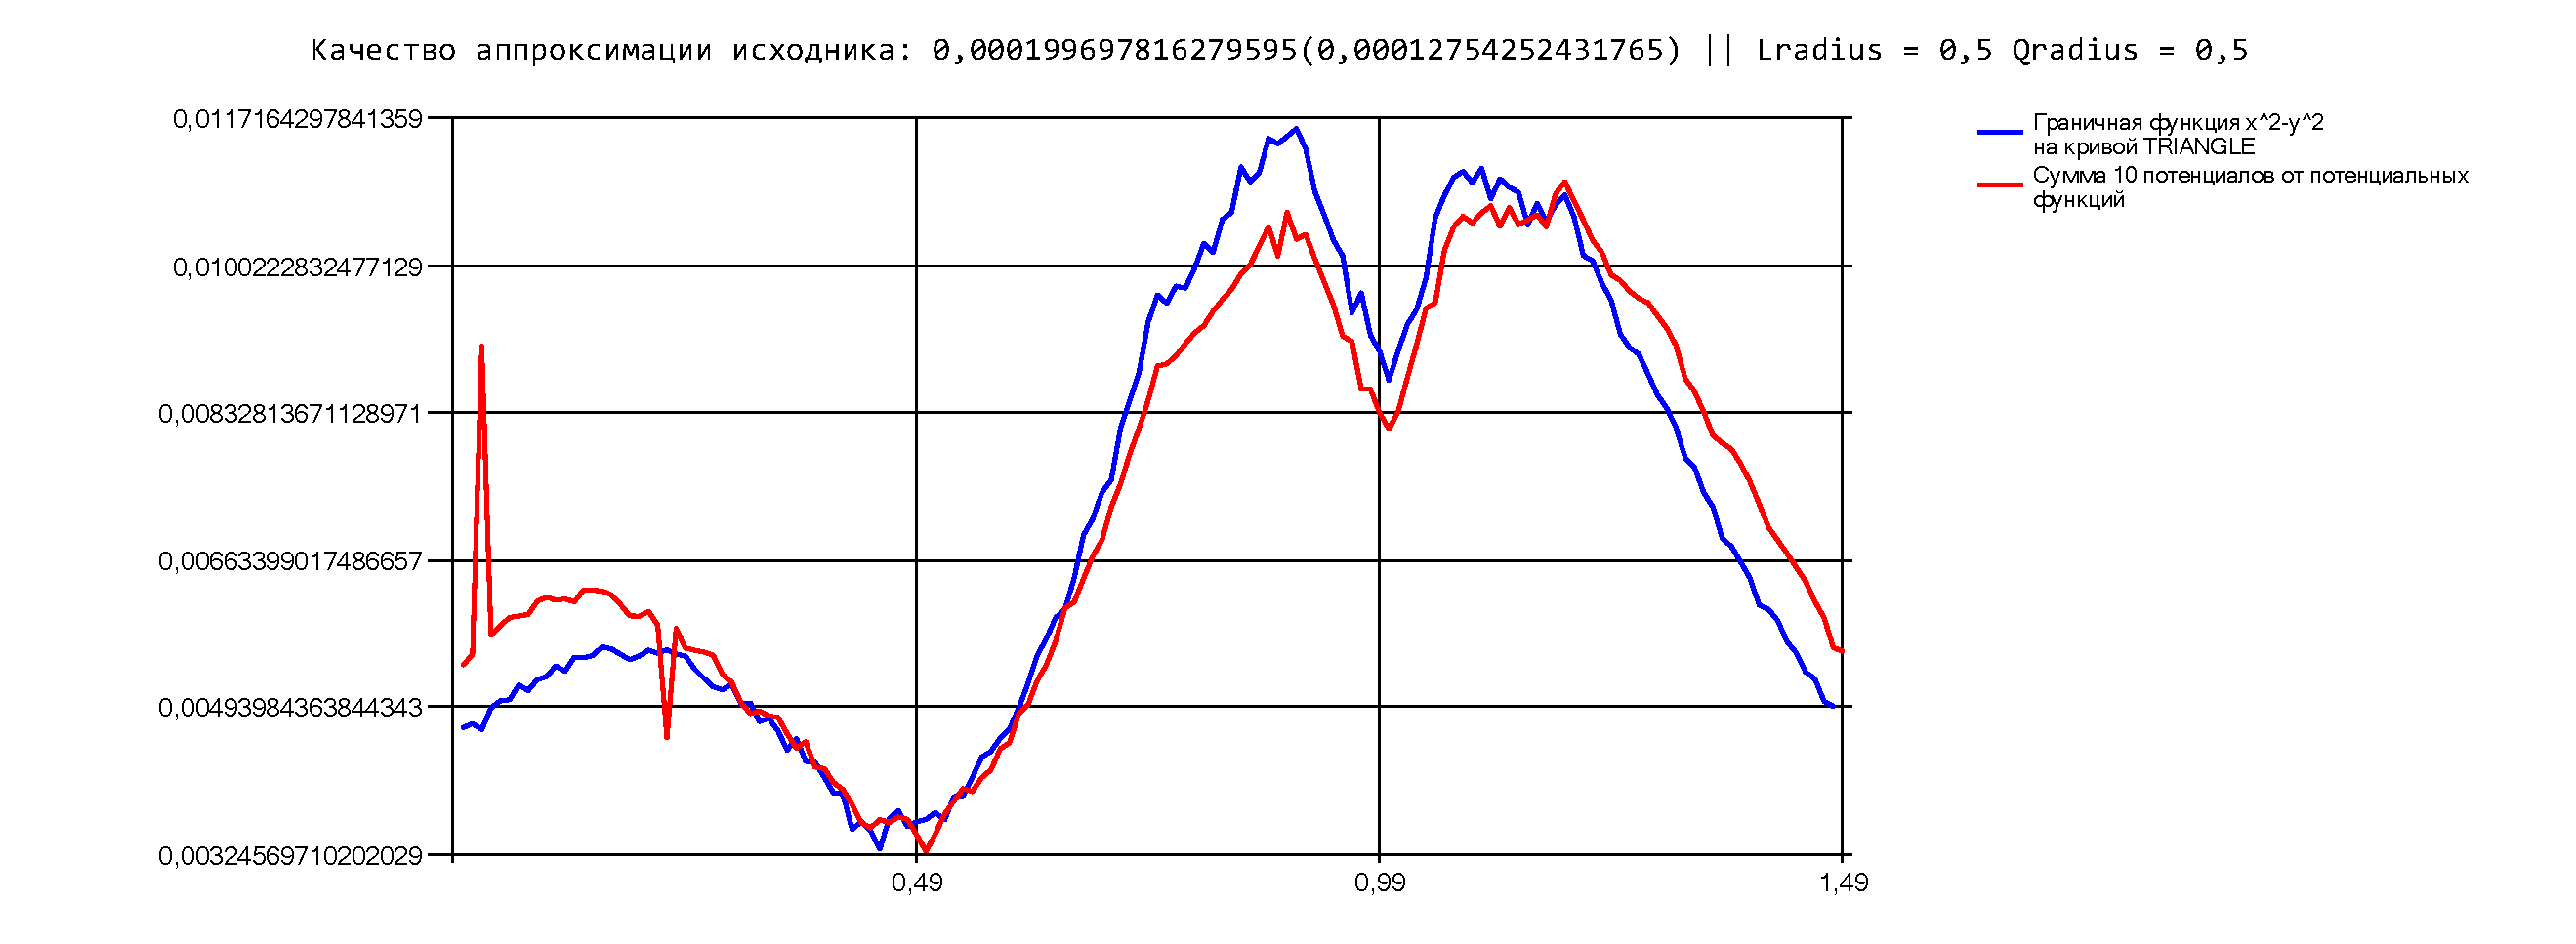
\includegraphics[width=0.8\linewidth]{v11.pdf} \\ для потенциала} 
        \end{minipage}} 
        \caption{Один из результатов работы алгоритма} 
        \label{hexampl2} 
        \end{figure}     
        
        \begin{figure}[h] 
          \center{\begin{minipage}[h]{\linewidth} 
          \center{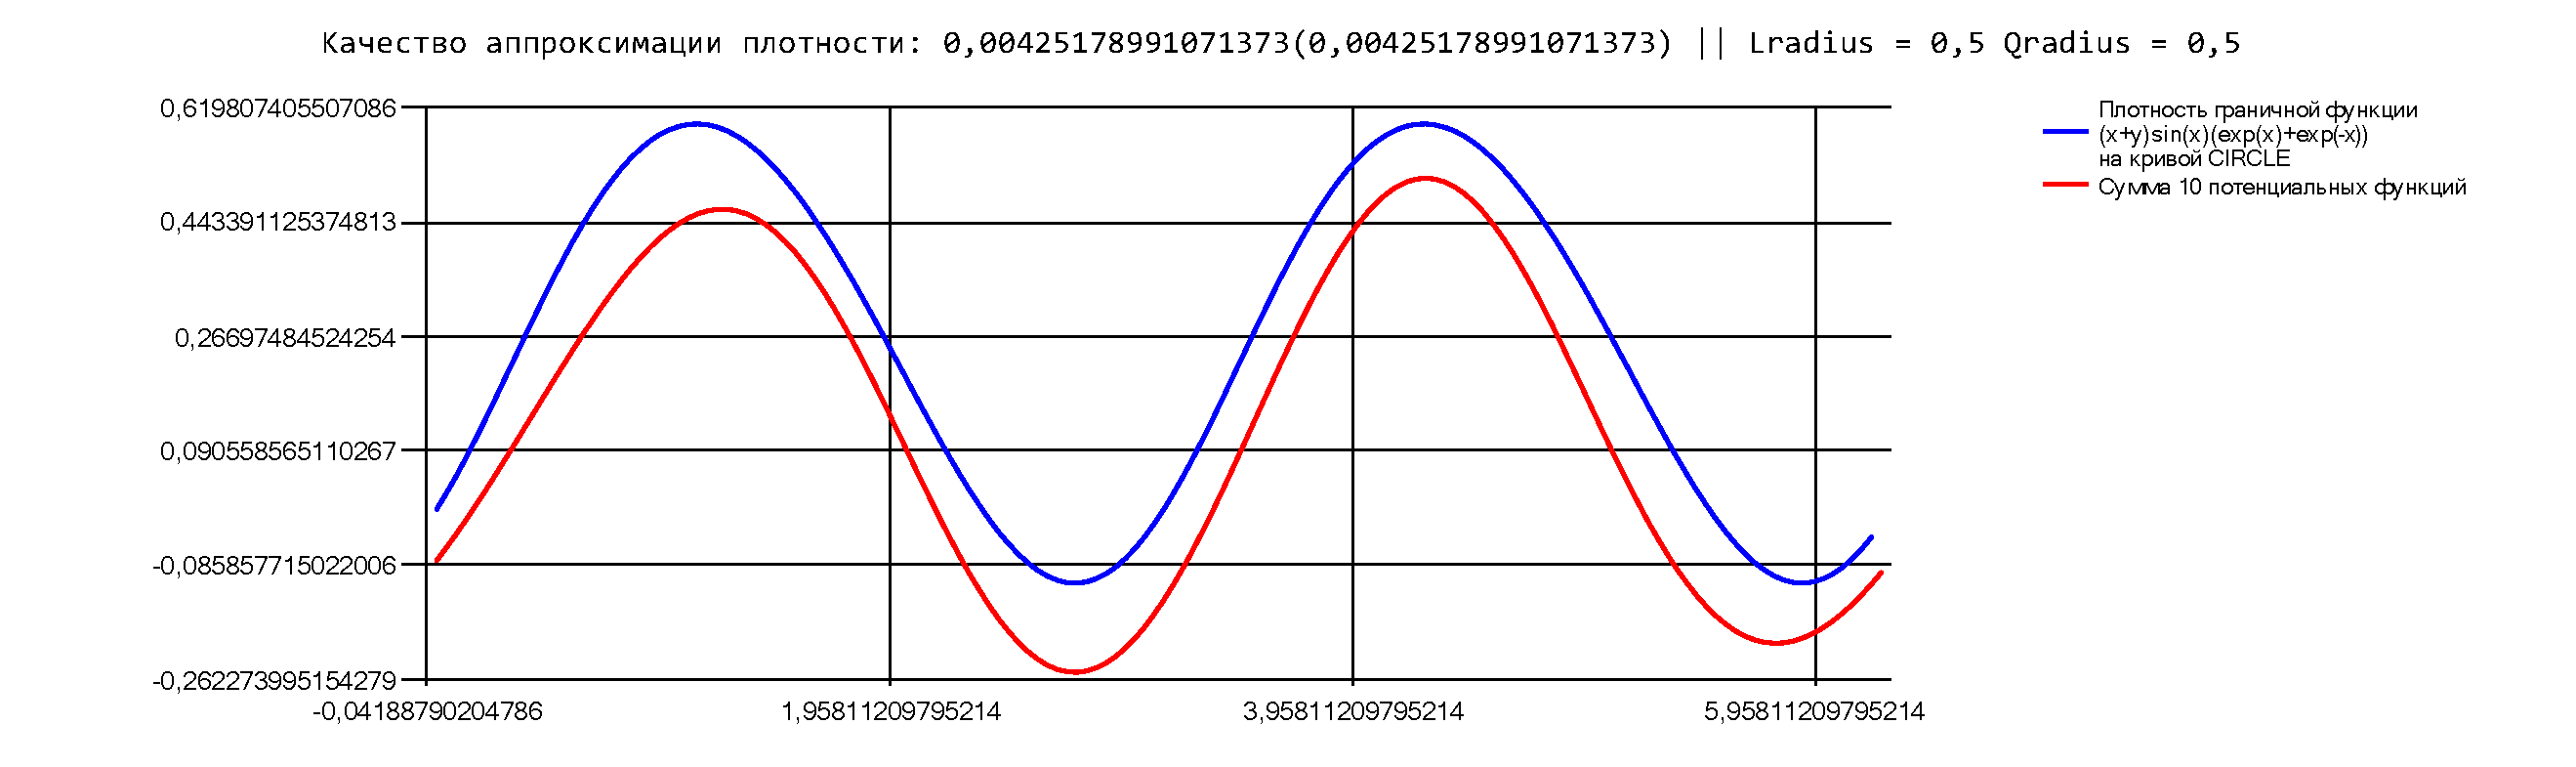
\includegraphics[width=0.8\linewidth]{d12.pdf} \\ для плотности} 
          \end{minipage}} 
          \vfill 
          \center{\begin{minipage}[h]{\linewidth} 
          \center{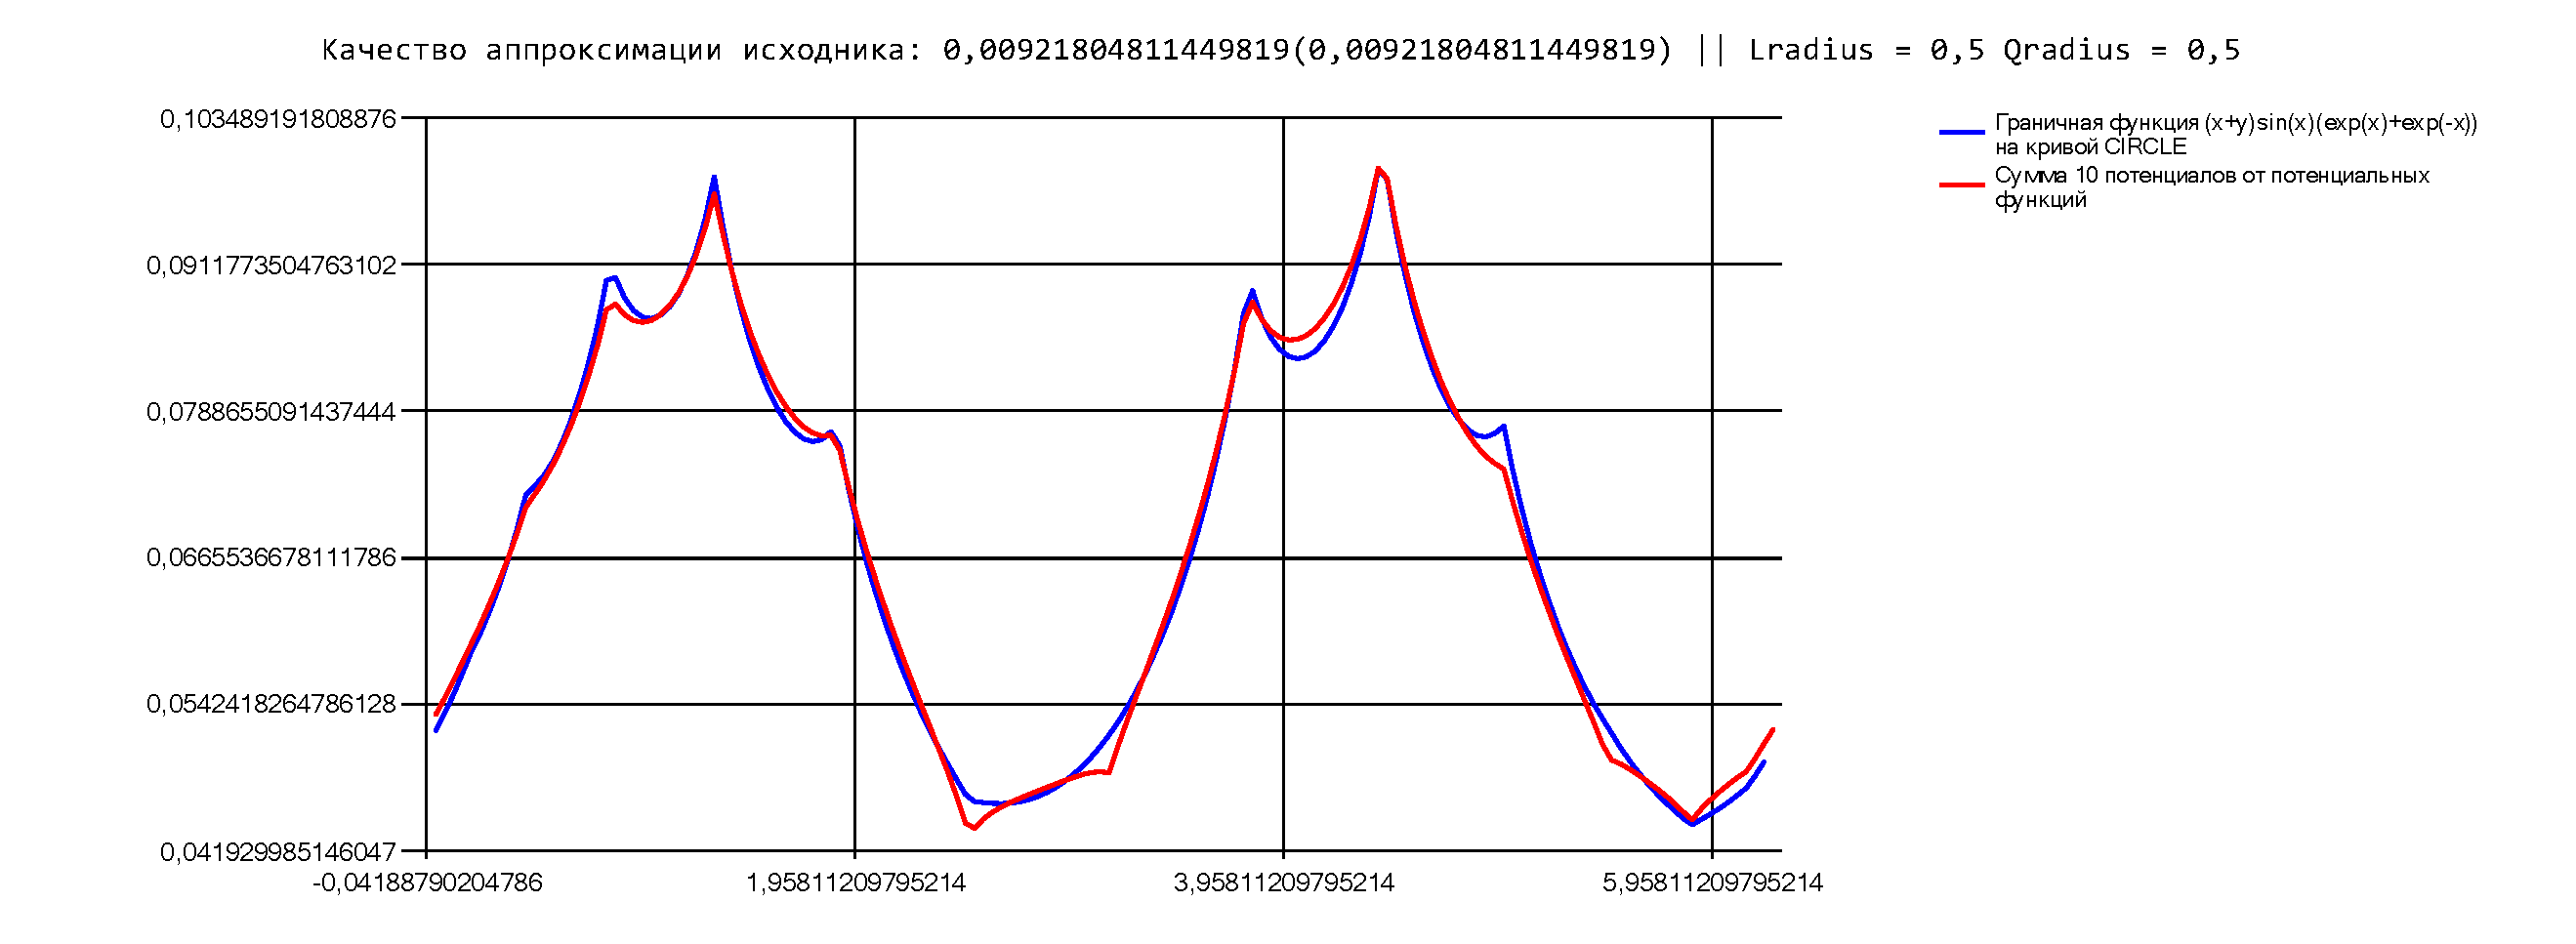
\includegraphics[width=0.8\linewidth]{v12.pdf} \\ для потенциала} 
          \end{minipage}} 
          \caption{Один из результатов работы алгоритма} 
          \label{ris:image1} 
          \end{figure}

          \begin{figure}[h] 
            \center{\begin{minipage}[h]{\linewidth} 
            \center{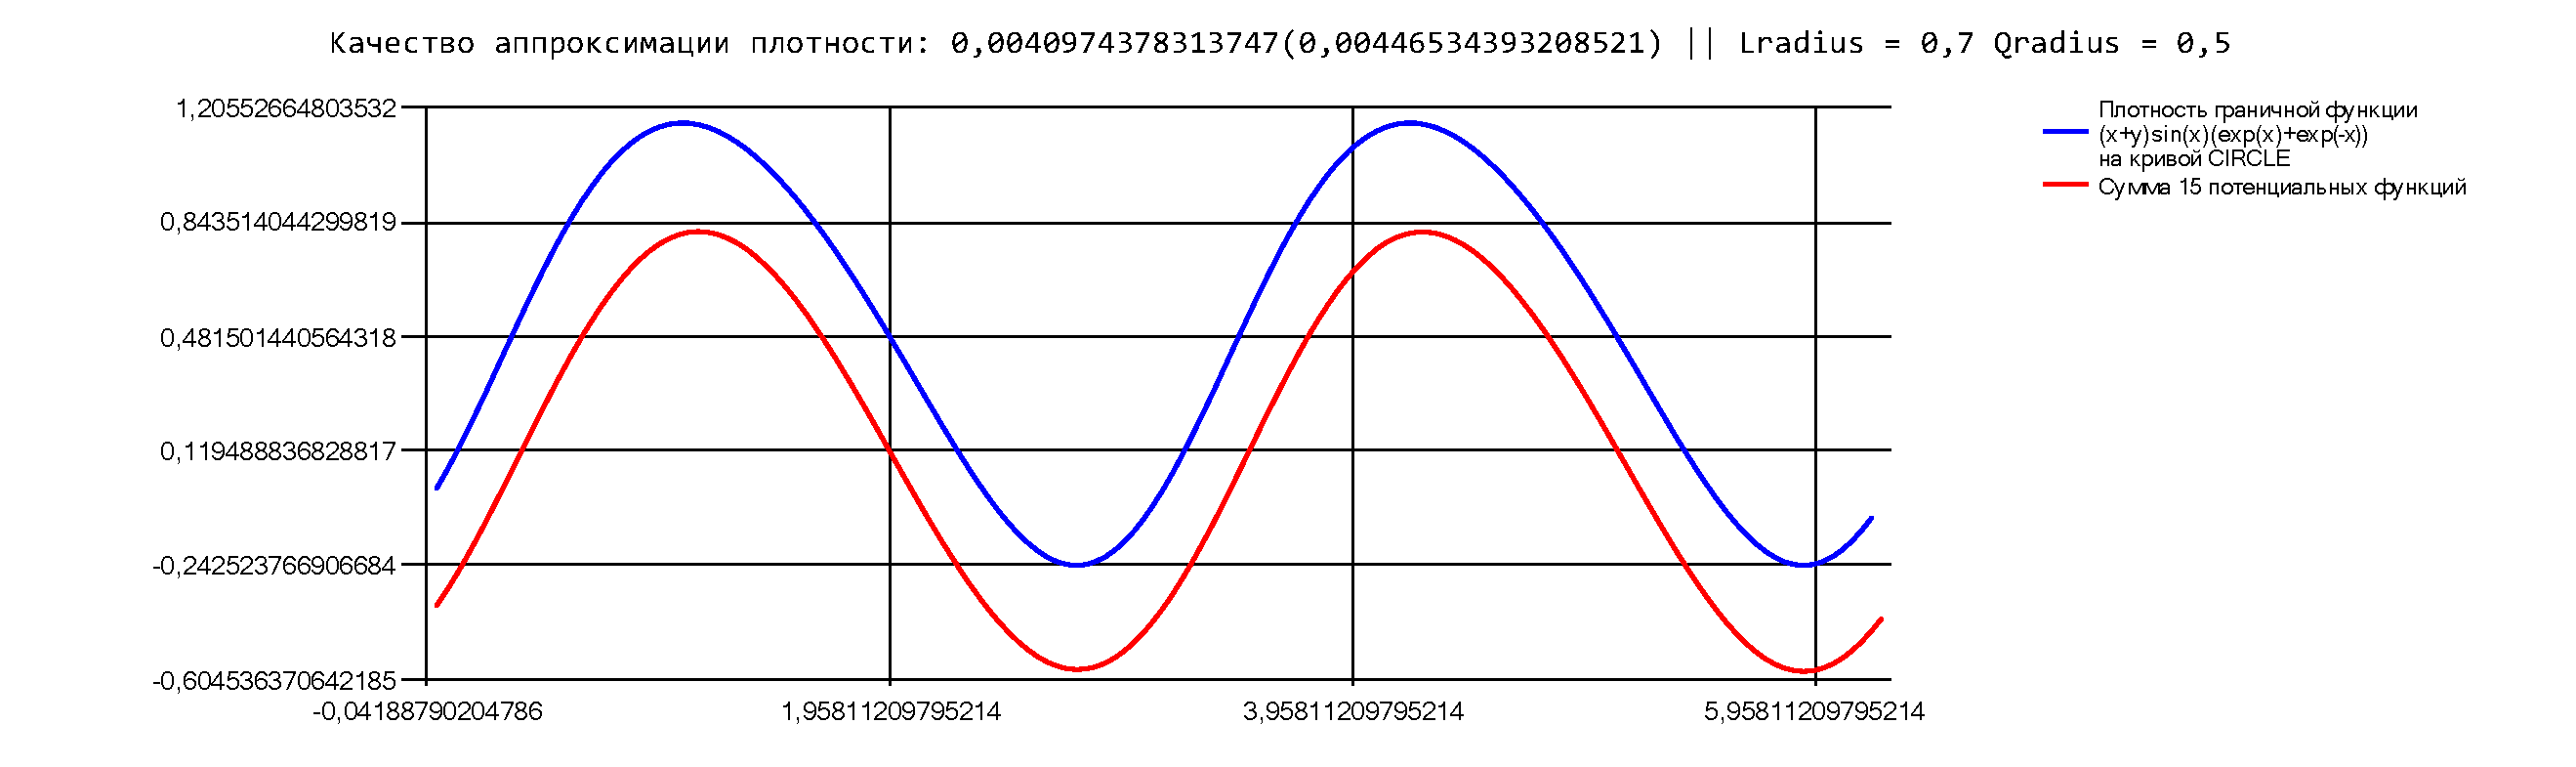
\includegraphics[width=0.8\linewidth]{d13.pdf} \\ для плотности} 
            \end{minipage}} 
            \vfill 
            \center{\begin{minipage}[h]{\linewidth} 
            \center{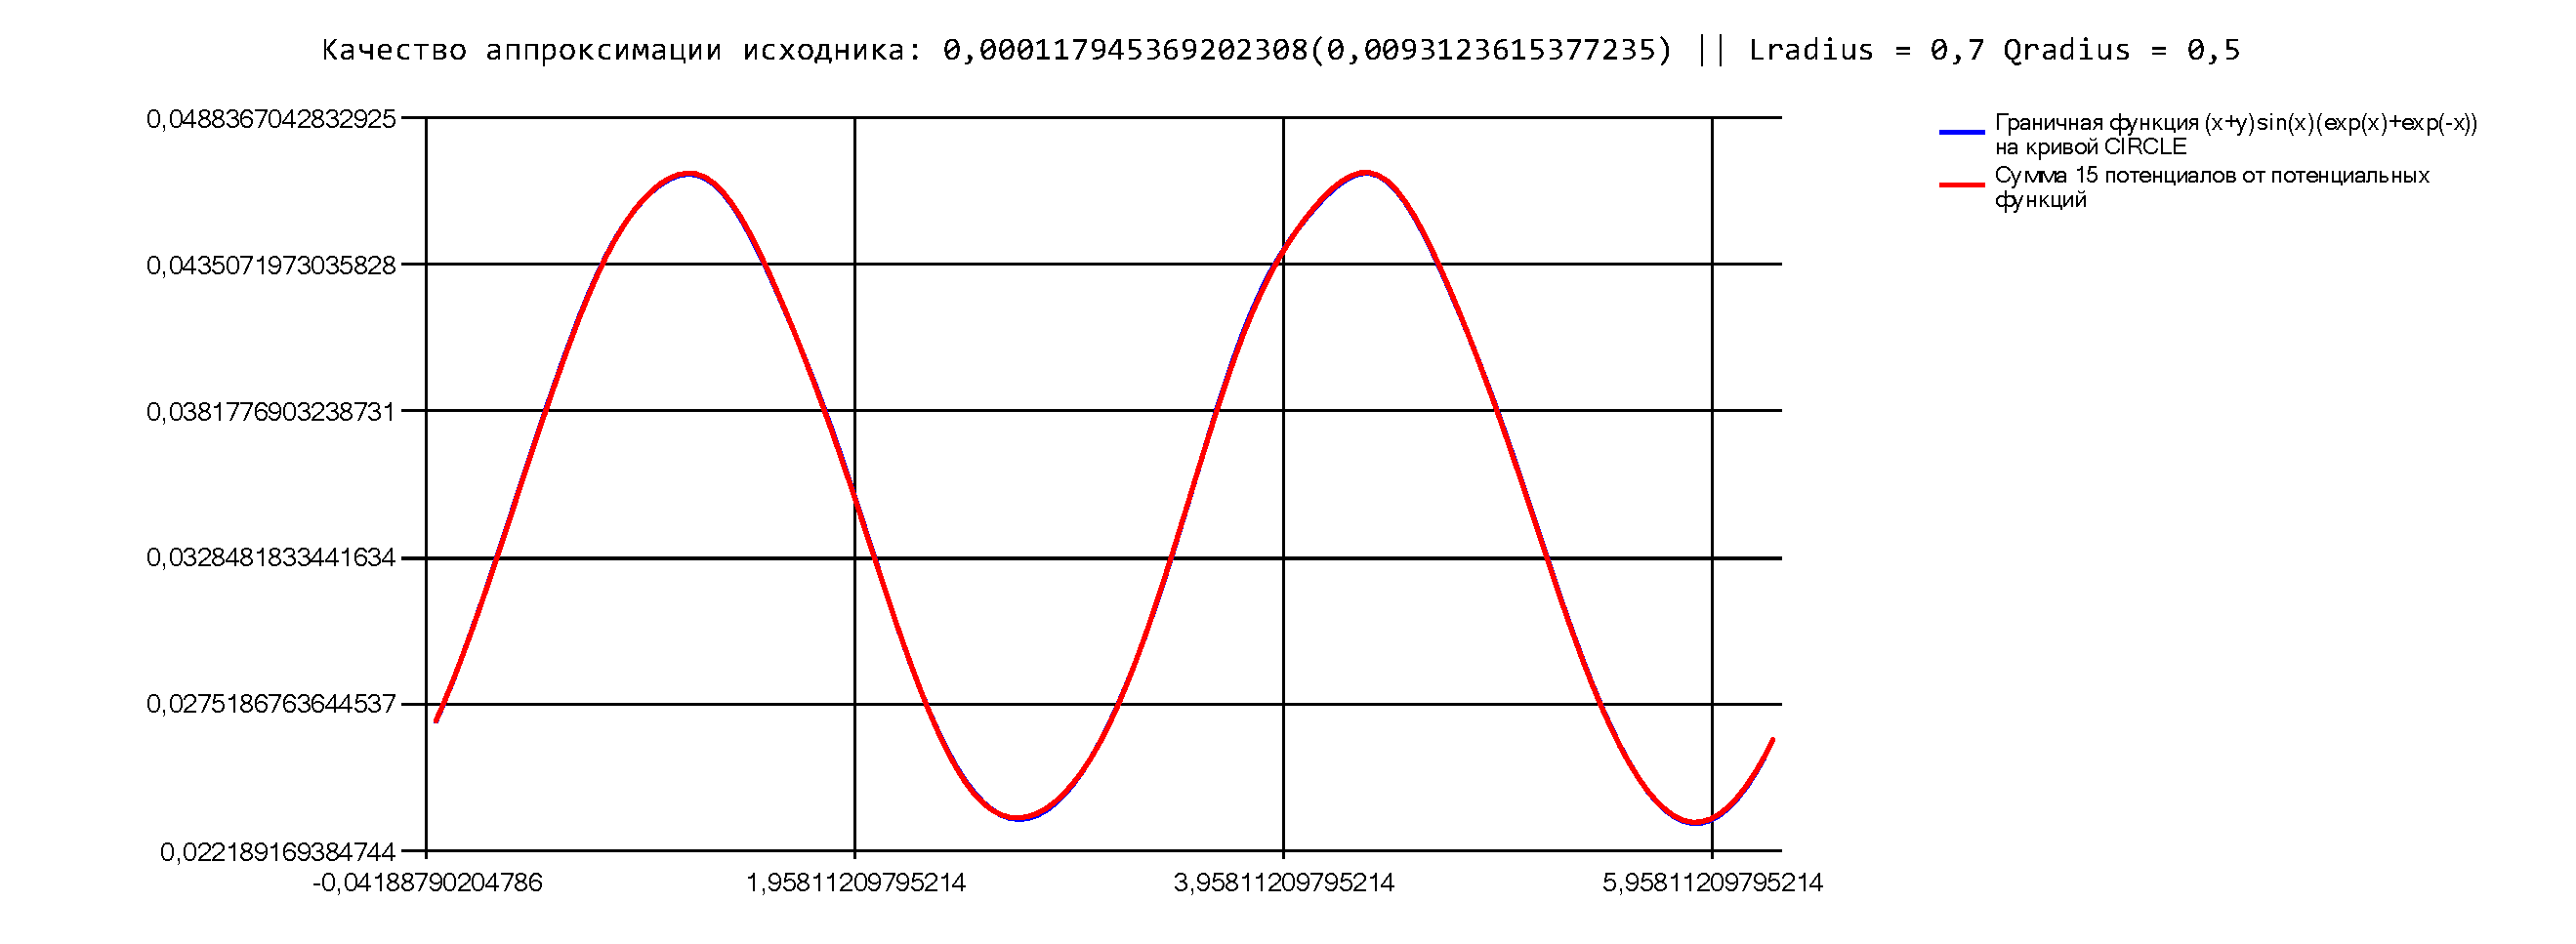
\includegraphics[width=0.8\linewidth]{v13.pdf} \\ для потенциала} 
            \end{minipage}} 
            \caption{Один из результатов работы алгоритма} 
            \label{p3} 
            \end{figure}

            \begin{figure}[h] 
              \center{\begin{minipage}[h]{\linewidth} 
              \center{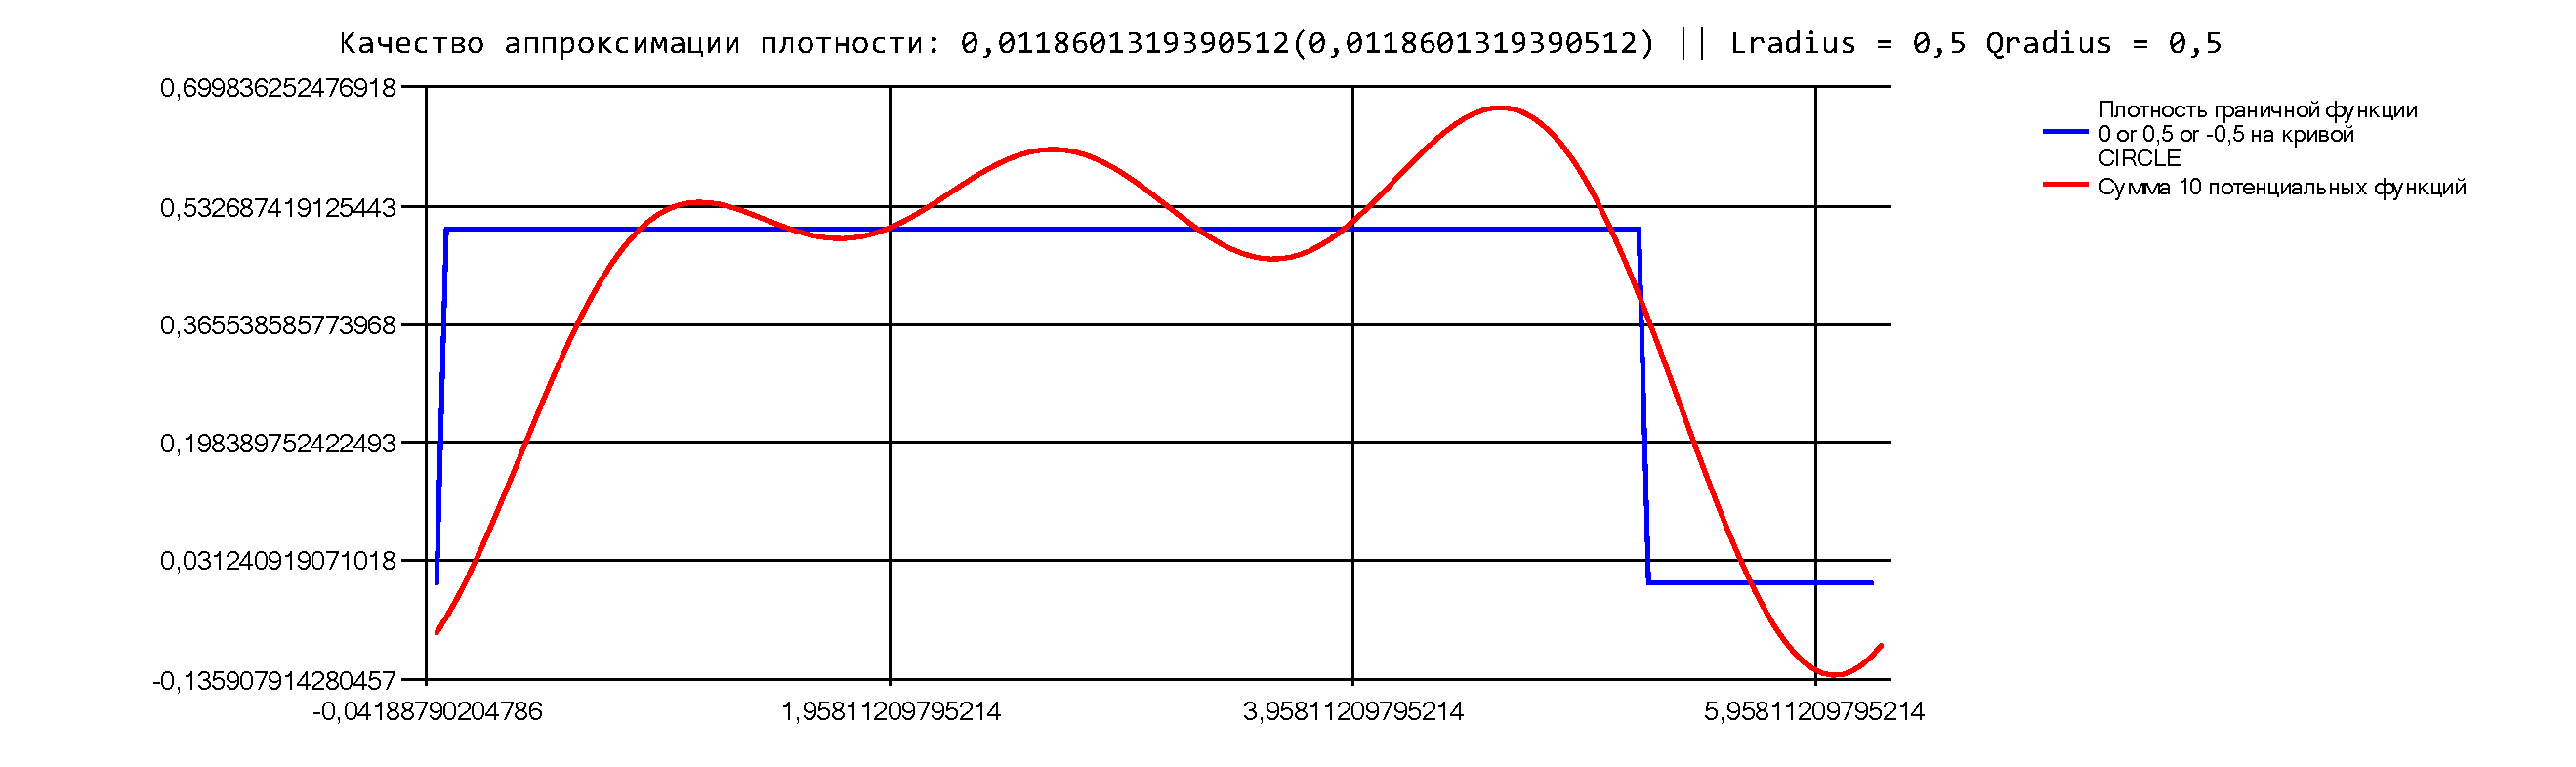
\includegraphics[width=0.8\linewidth]{d14.pdf} \\ для плотности} 
              \end{minipage}} 
              \vfill 
              \center{\begin{minipage}[h]{\linewidth} 
              \center{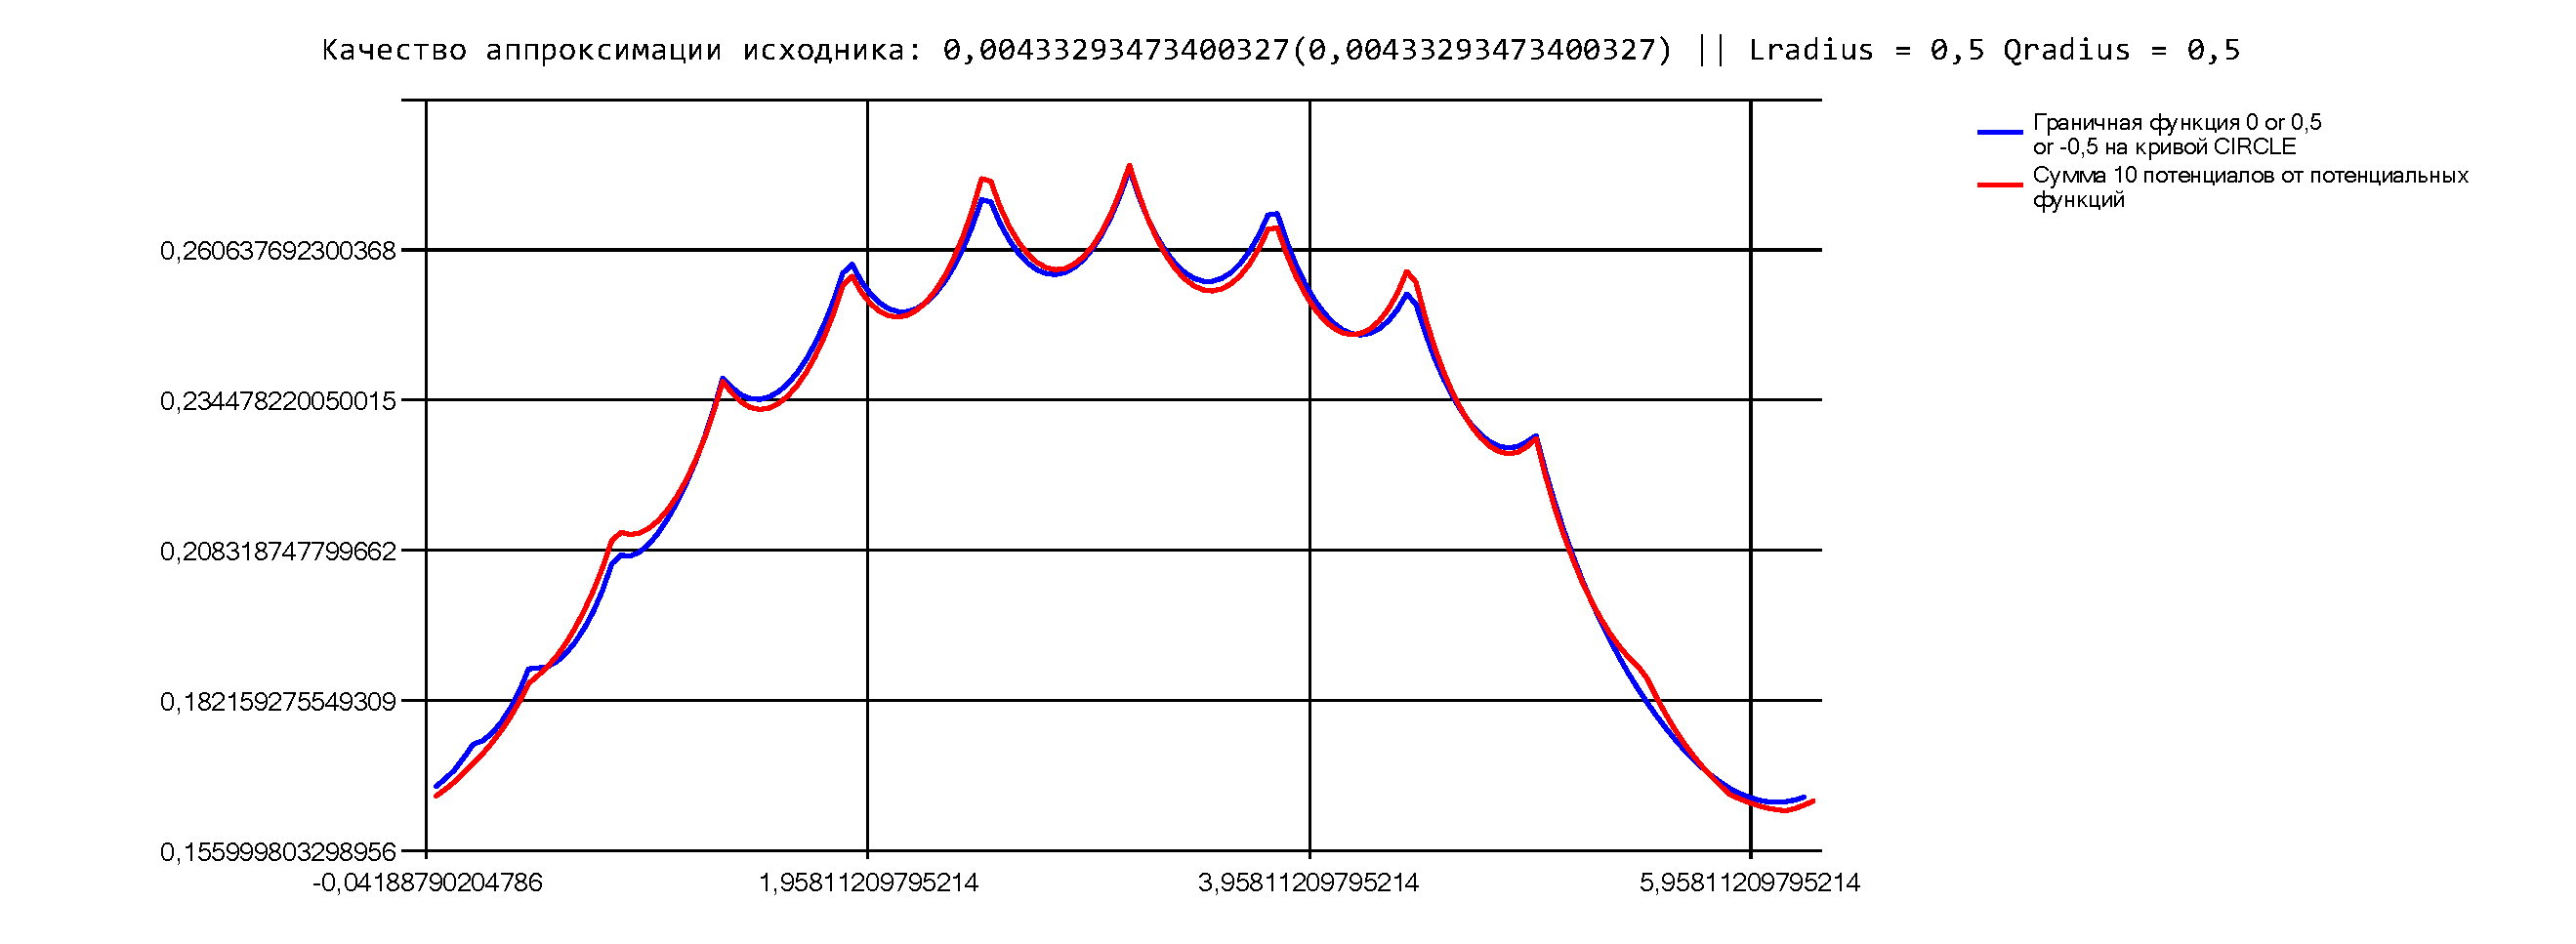
\includegraphics[width=0.8\linewidth]{v14.pdf} \\ для потенциала} 
              \end{minipage}} 
              \caption{Один из результатов работы алгоритма} 
              \label{p4} 
              \end{figure}

              \begin{figure}[h] 
                \center{\begin{minipage}[h]{\linewidth} 
                \center{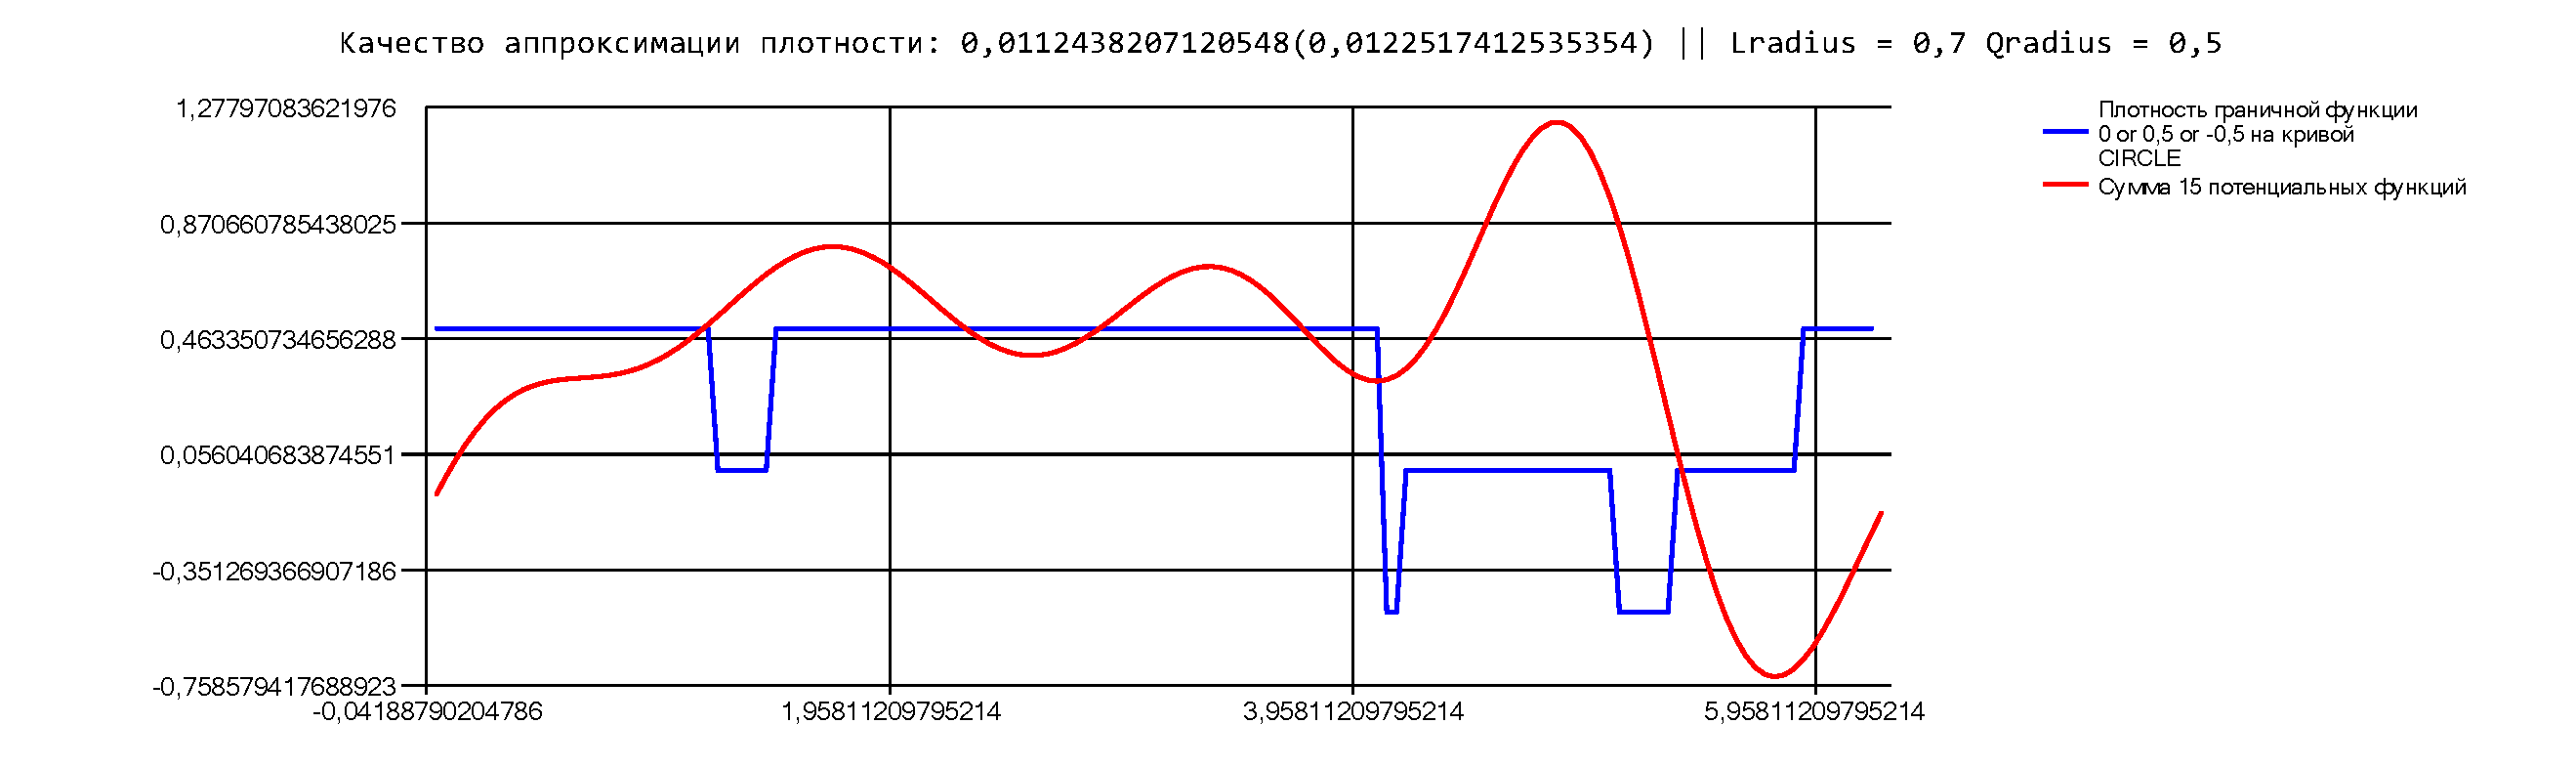
\includegraphics[width=0.8\linewidth]{d15.pdf} \\ для плотности} 
                \end{minipage}} 
                \vfill 
                \center{\begin{minipage}[h]{\linewidth} 
                \center{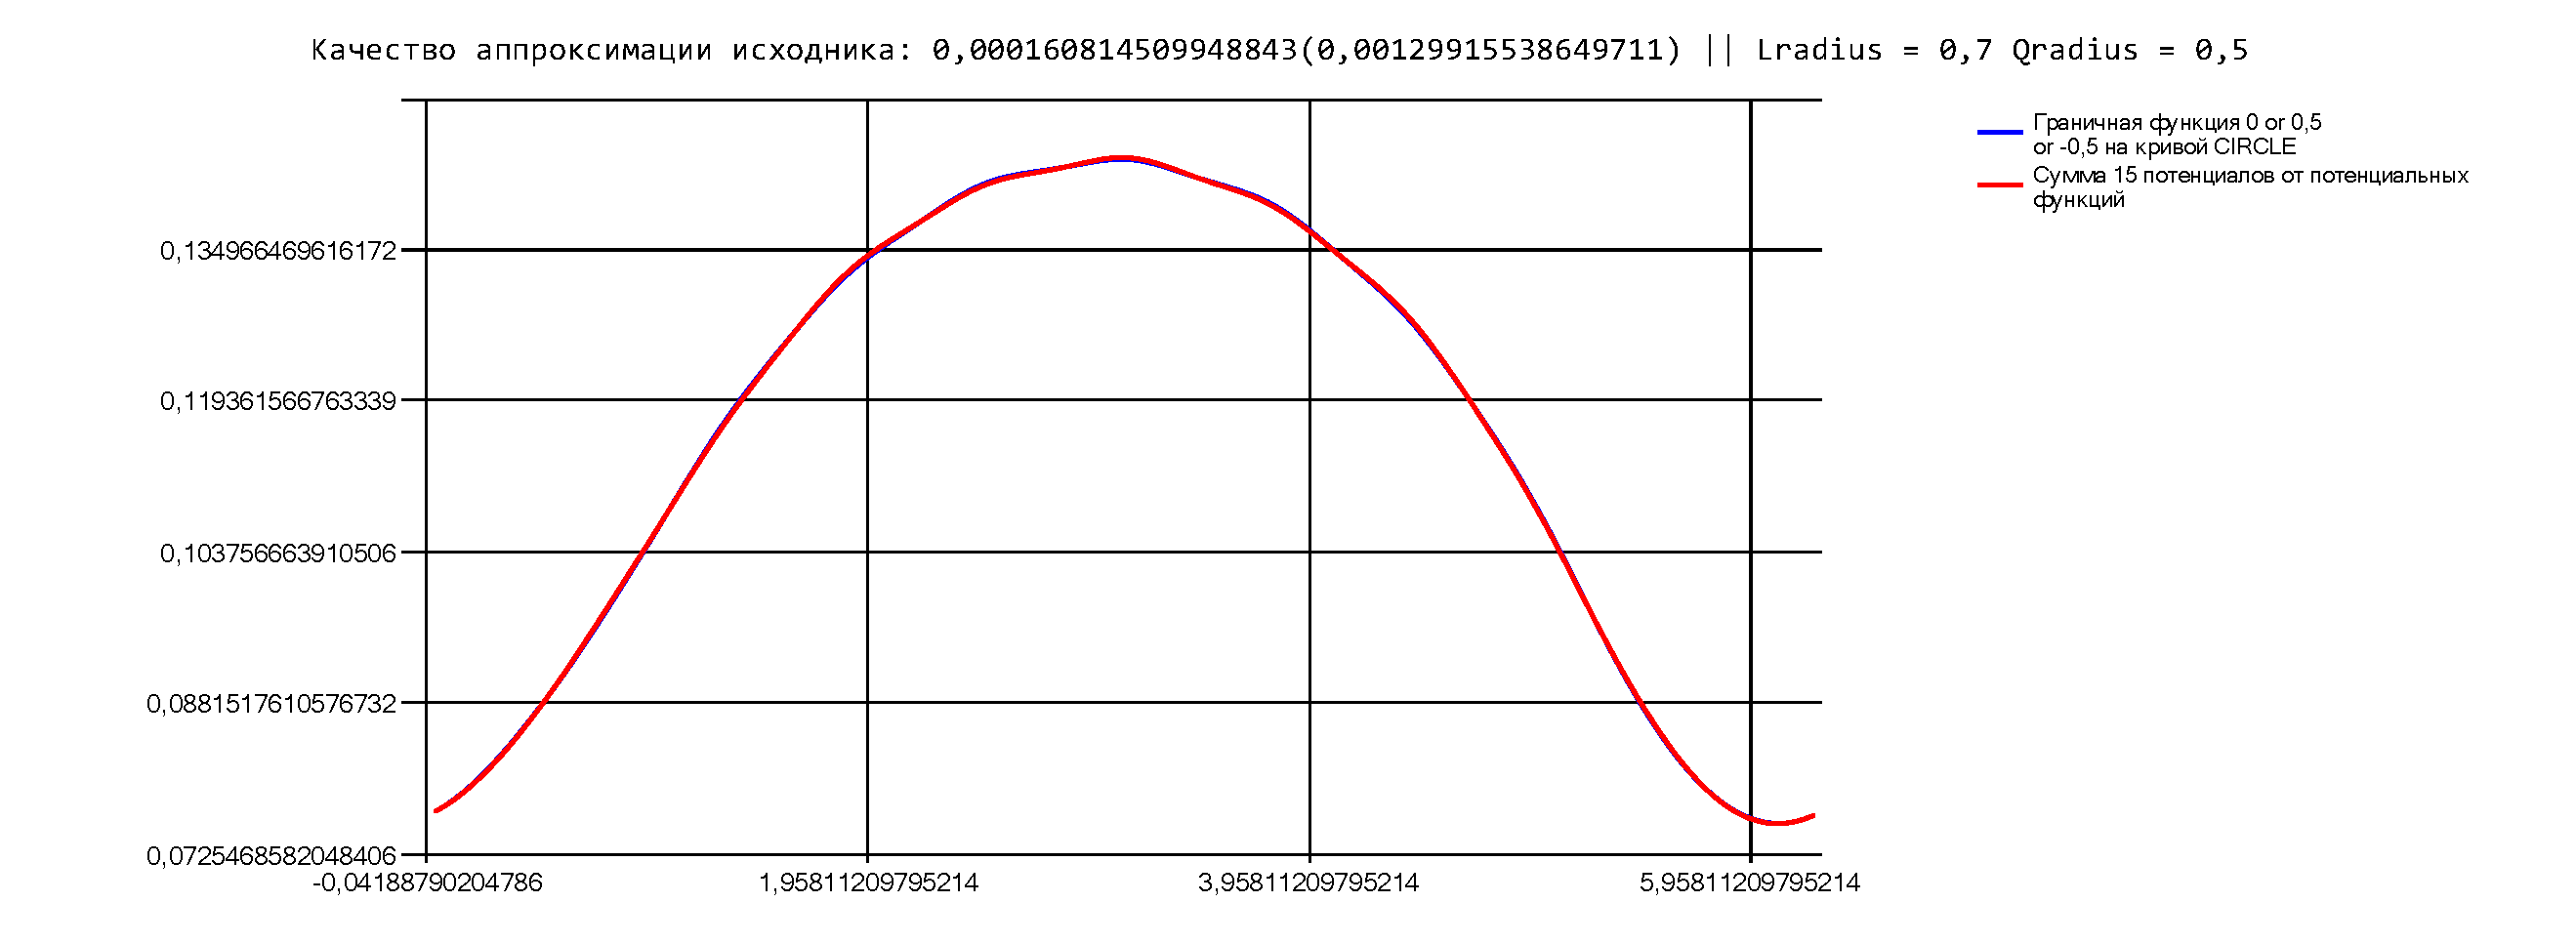
\includegraphics[width=0.8\linewidth]{v15.pdf} \\ для потенциала} 
                \end{minipage}} 
                \caption{Один из результатов работы алгоритма} 
                \label{p5} 
                \end{figure}

                \begin{figure}[h] 
                  \center{\begin{minipage}[h]{\linewidth} 
                  \center{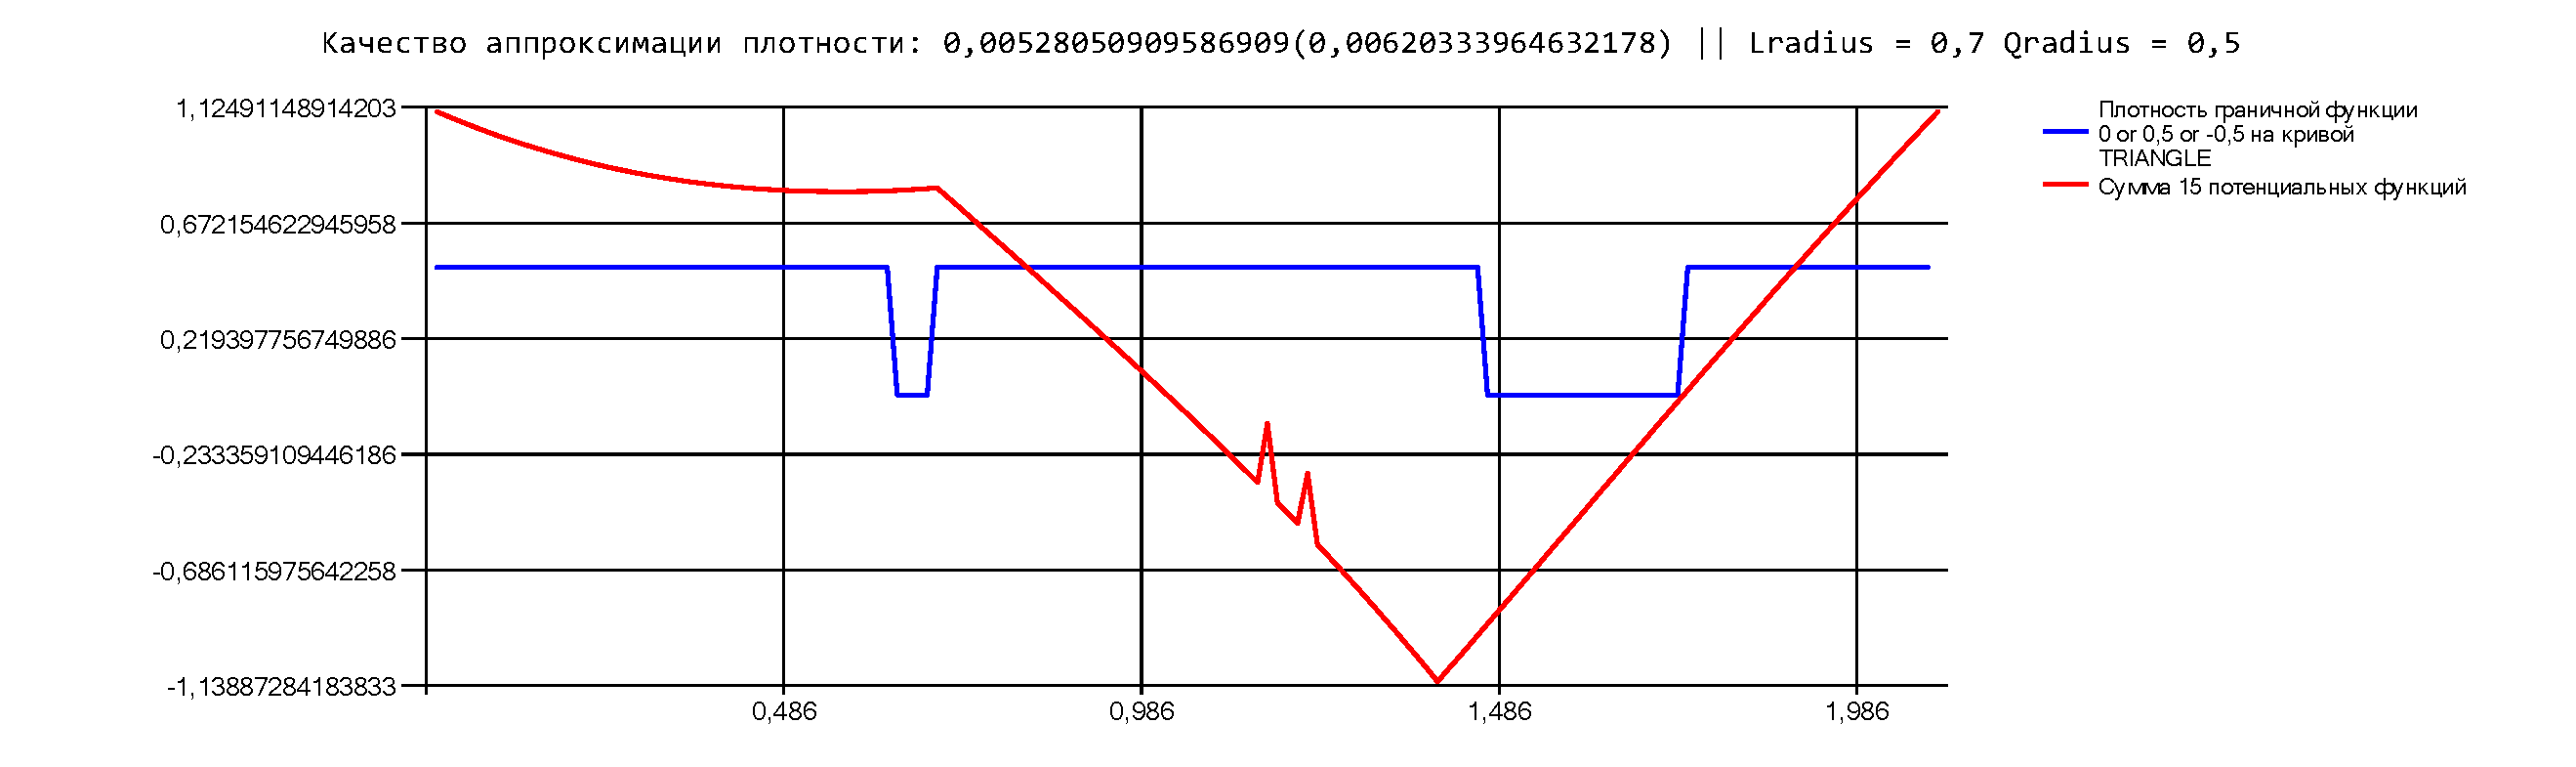
\includegraphics[width=0.8\linewidth]{d16.pdf} \\ для плотности} 
                  \end{minipage}} 
                  \vfill 
                  \center{\begin{minipage}[h]{\linewidth} 
                  \center{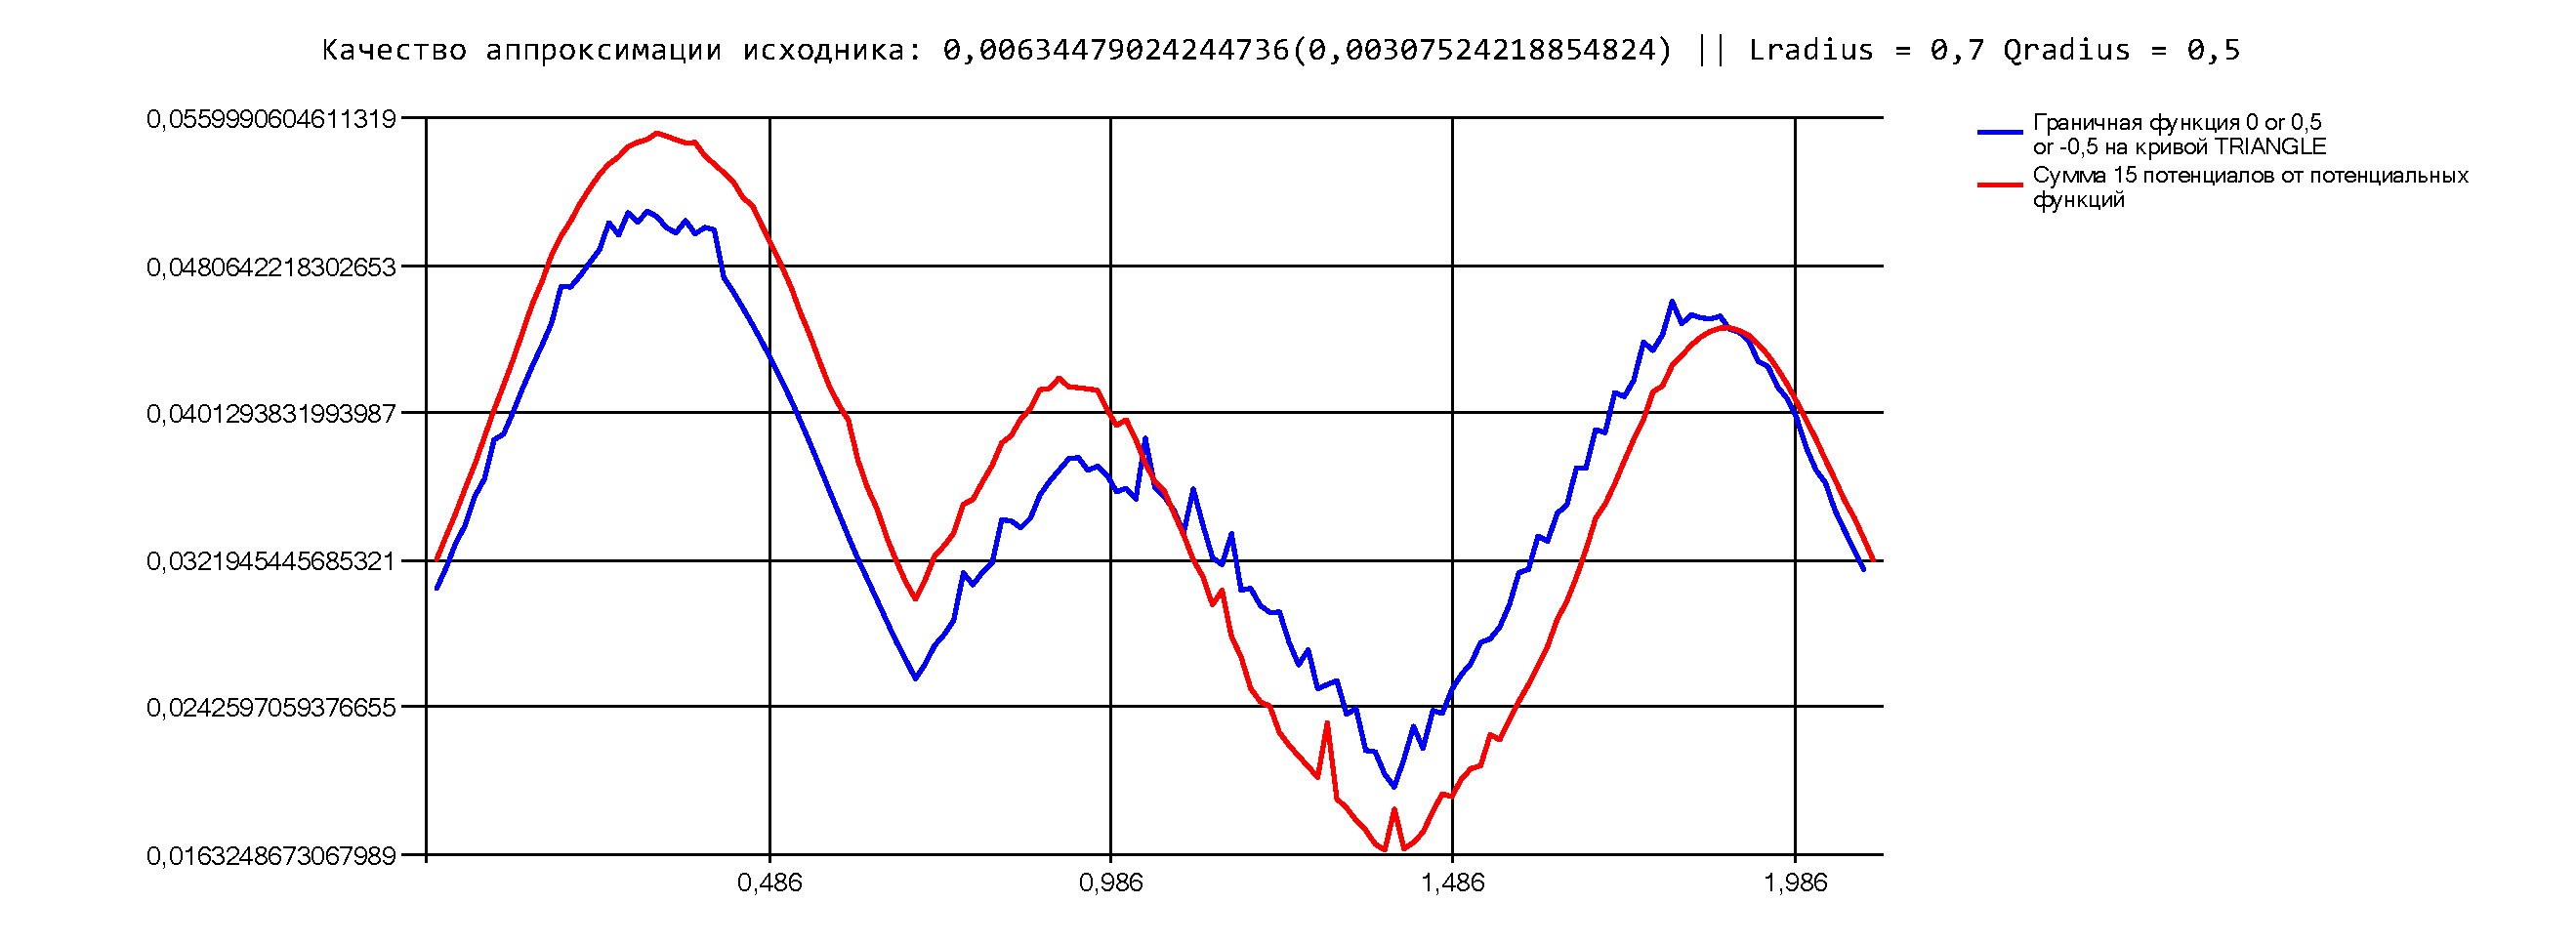
\includegraphics[width=0.8\linewidth]{v16.pdf} \\ для потенциала} 
                  \end{minipage}} 
                  \caption{Один из результатов работы алгоритма} 
                  \label{ris:image1} 
                  \end{figure}


                  \begin{figure}[h] 
                    \center{\begin{minipage}[h]{\linewidth} 
                    \center{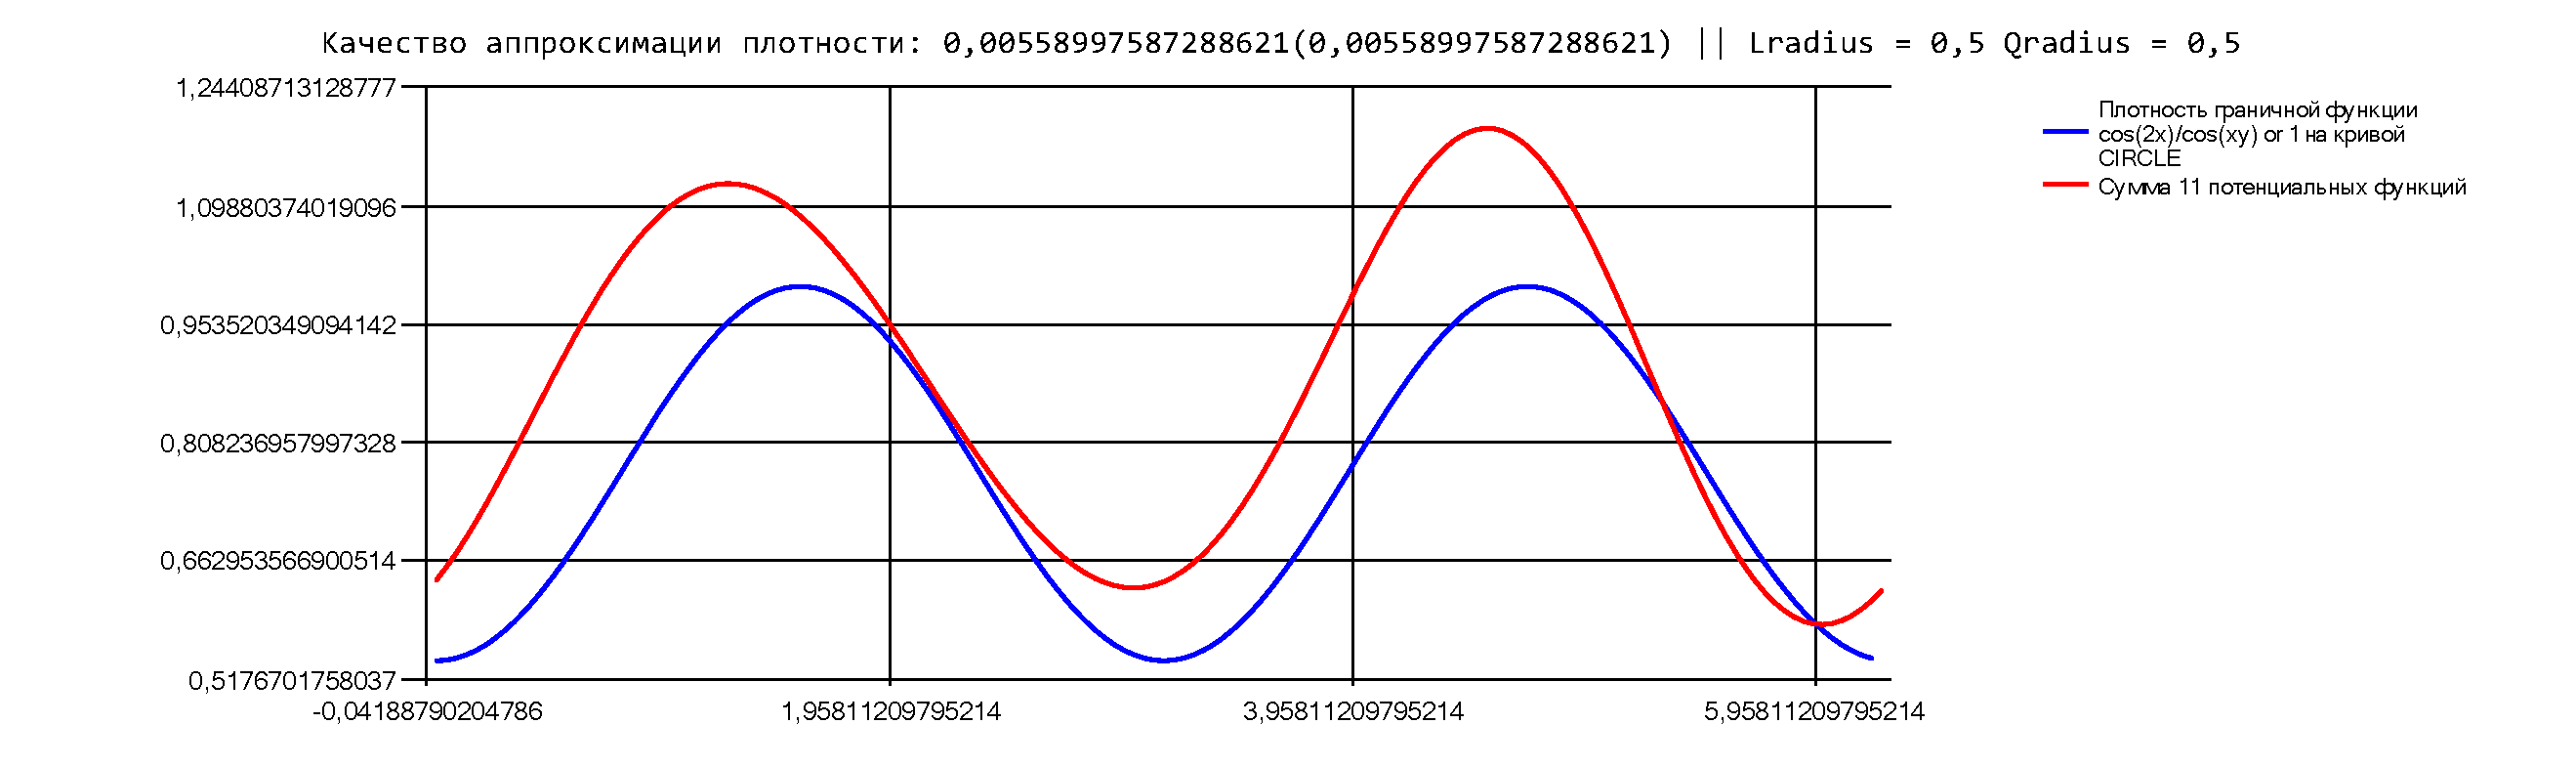
\includegraphics[width=0.8\linewidth]{d17.pdf} \\ для плотности} 
                    \end{minipage}} 
                    \vfill 
                    \center{\begin{minipage}[h]{\linewidth} 
                    \center{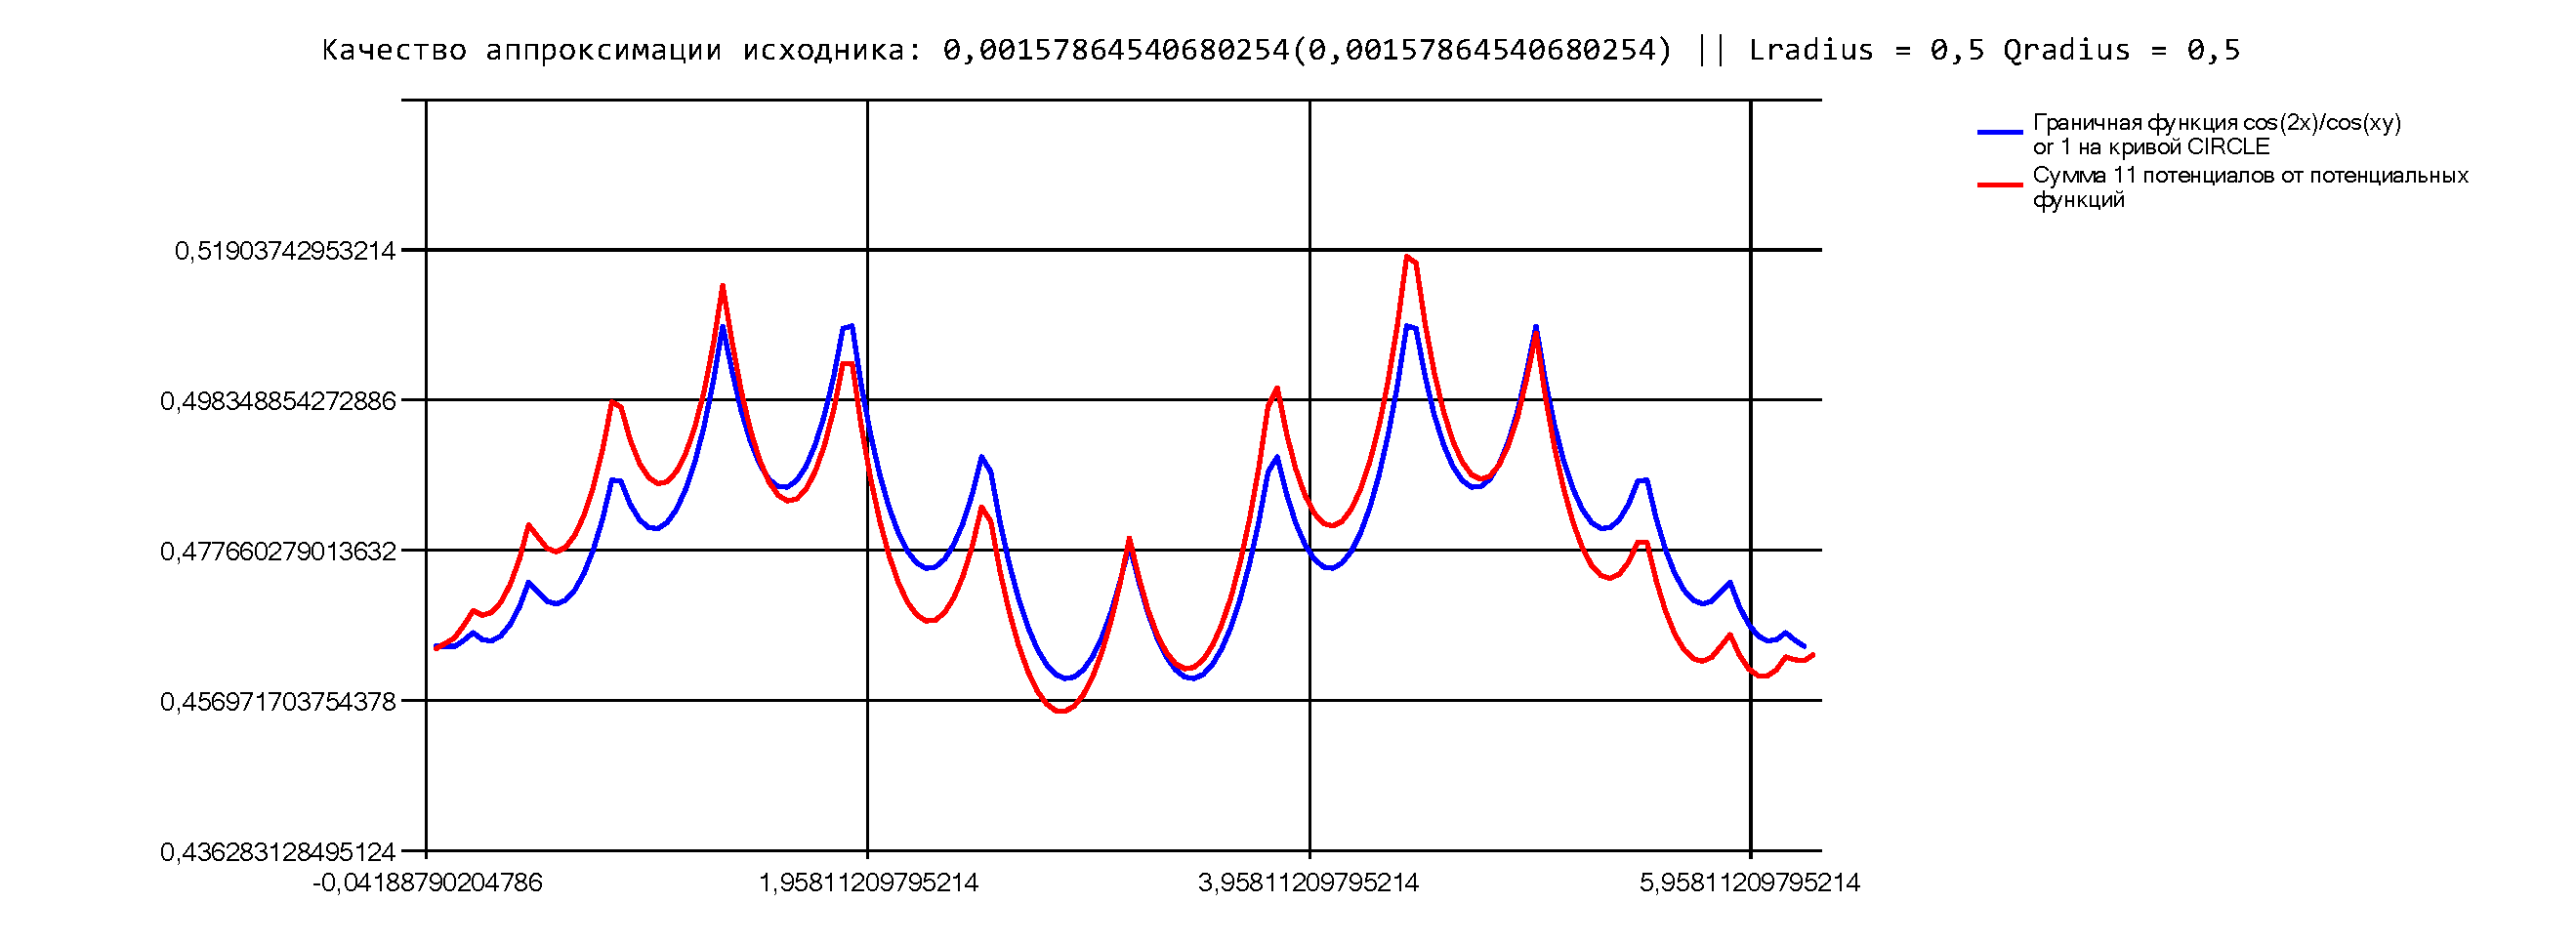
\includegraphics[width=0.8\linewidth]{v17.pdf} \\ для потенциала} 
                    \end{minipage}} 
                    \caption{Один из результатов работы алгоритма} 
                    \label{ris:image1} 
                    \end{figure}

                    \begin{figure}[h] 
                      \center{\begin{minipage}[h]{\linewidth} 
                      \center{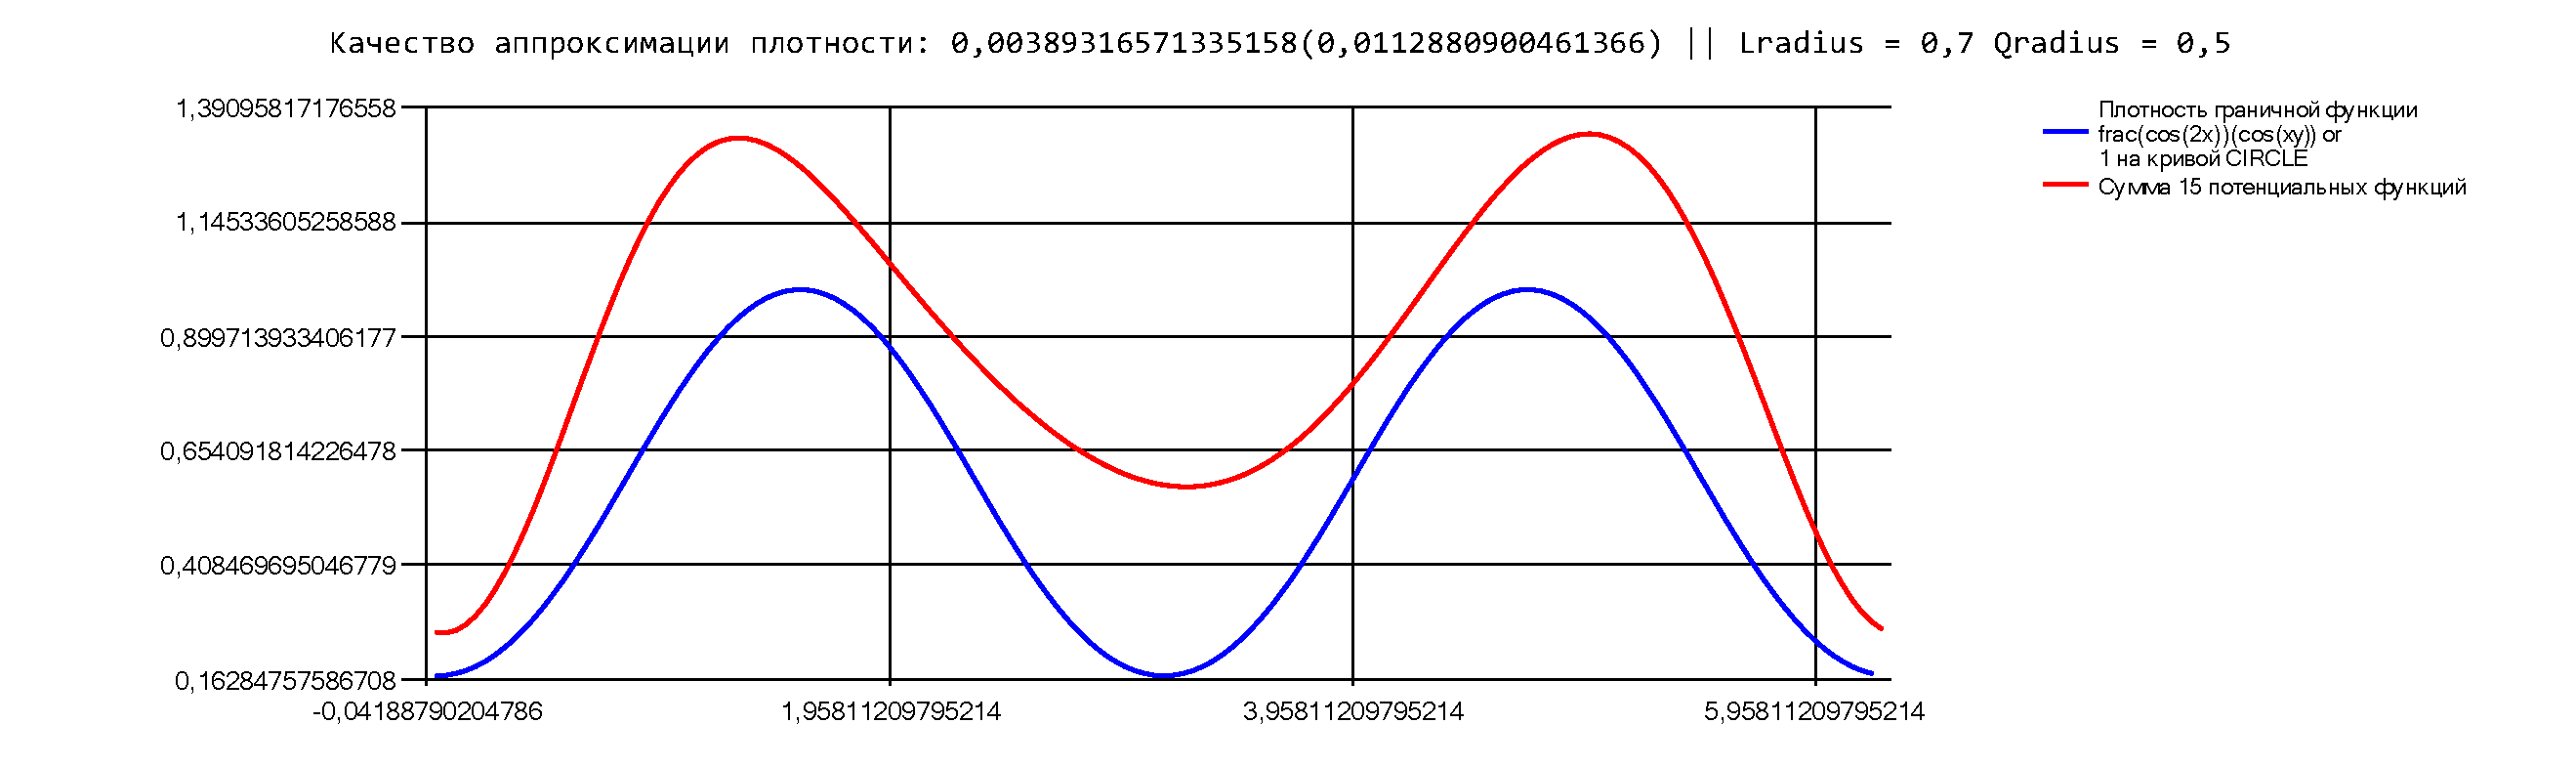
\includegraphics[width=0.8\linewidth]{d18.pdf} \\ для плотности} 
                      \end{minipage}} 
                      \vfill 
                      \center{\begin{minipage}[h]{\linewidth} 
                      \center{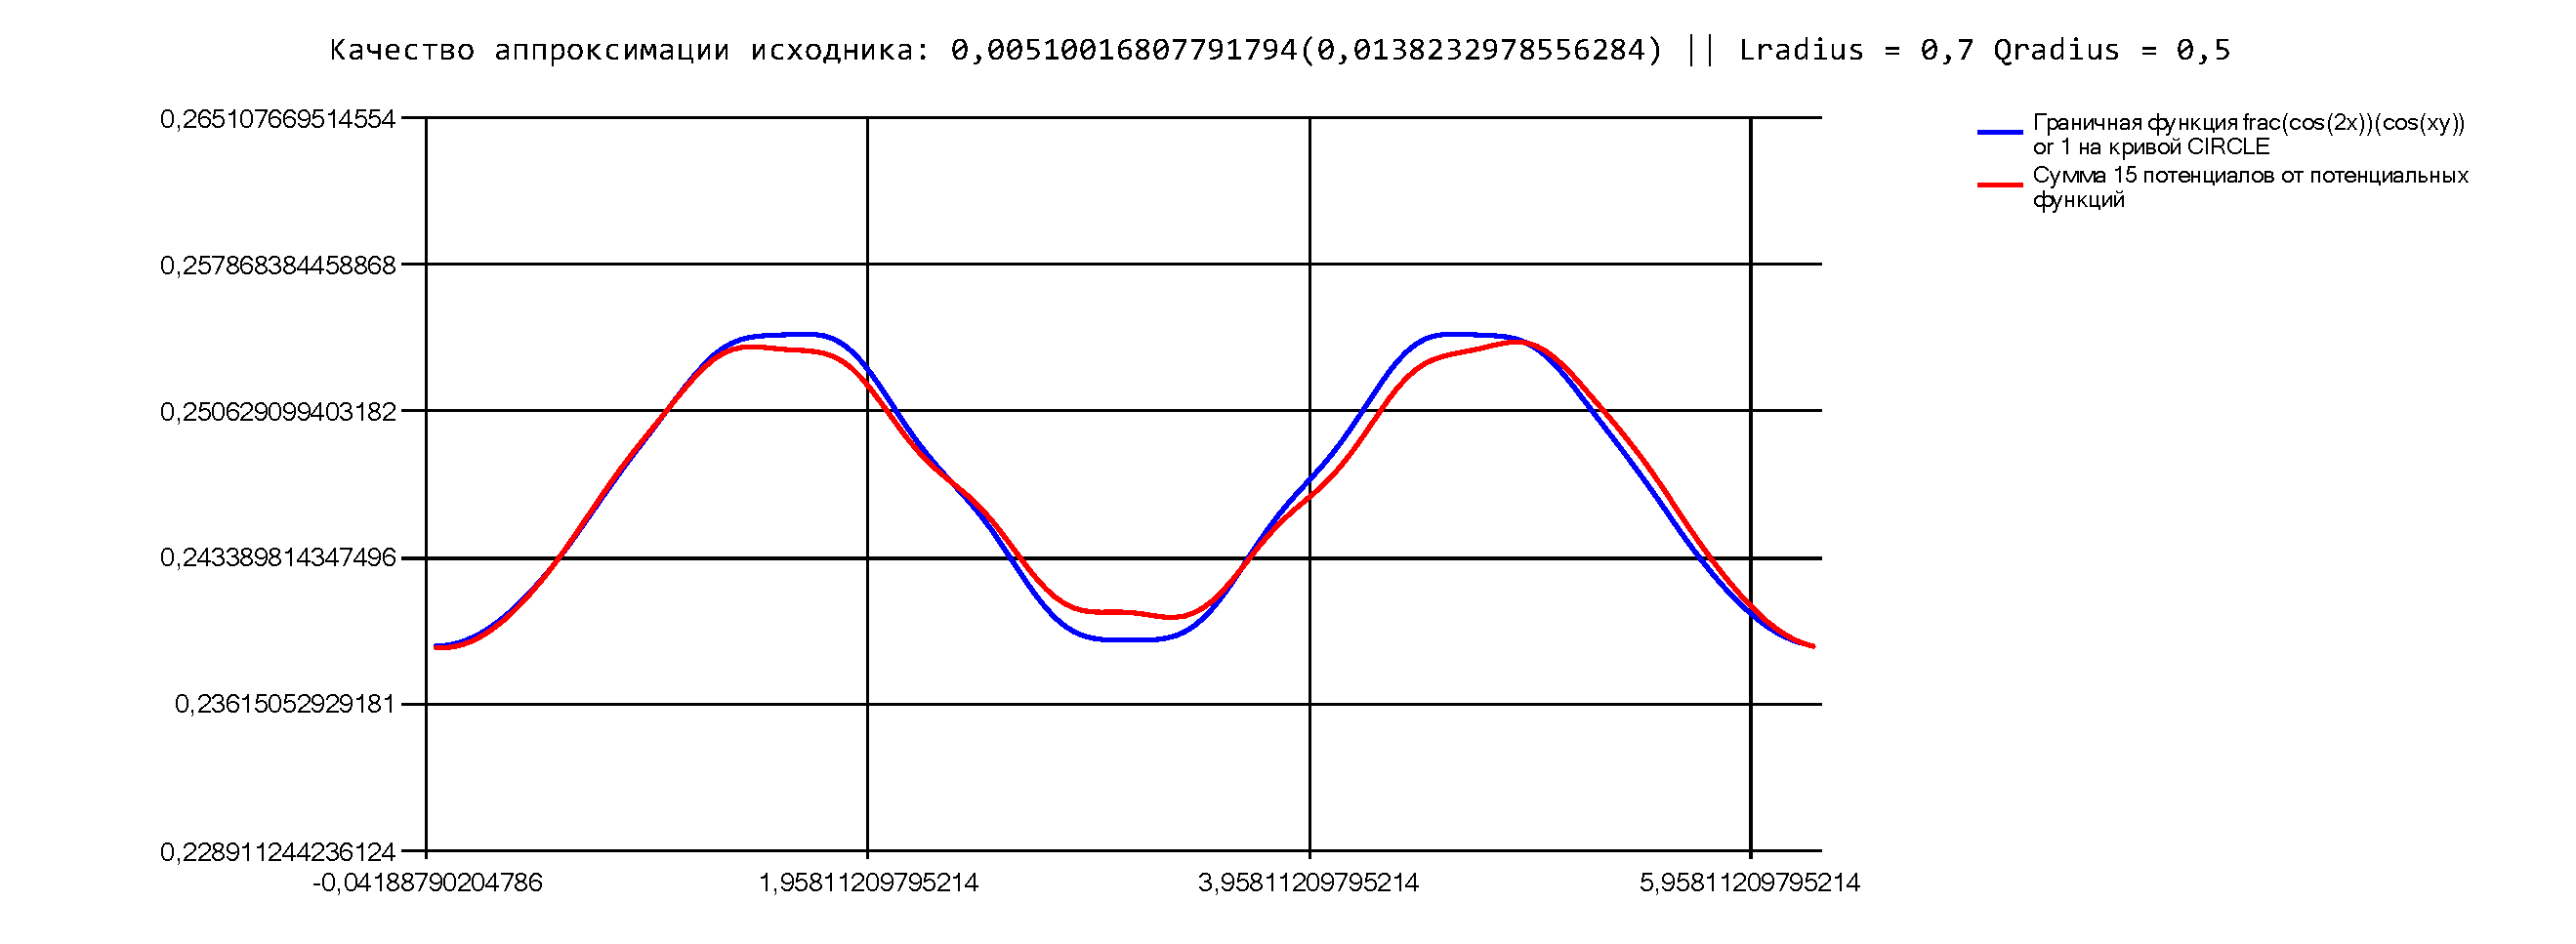
\includegraphics[width=0.8\linewidth]{v18.pdf} \\ для потенциала} 
                      \end{minipage}} 
                      \caption{Один из результатов работы алгоритма} 
                      \label{ris:image1} 
                      \end{figure}


                      \begin{figure}[h] 
                        \center{\begin{minipage}[h]{\linewidth} 
                        \center{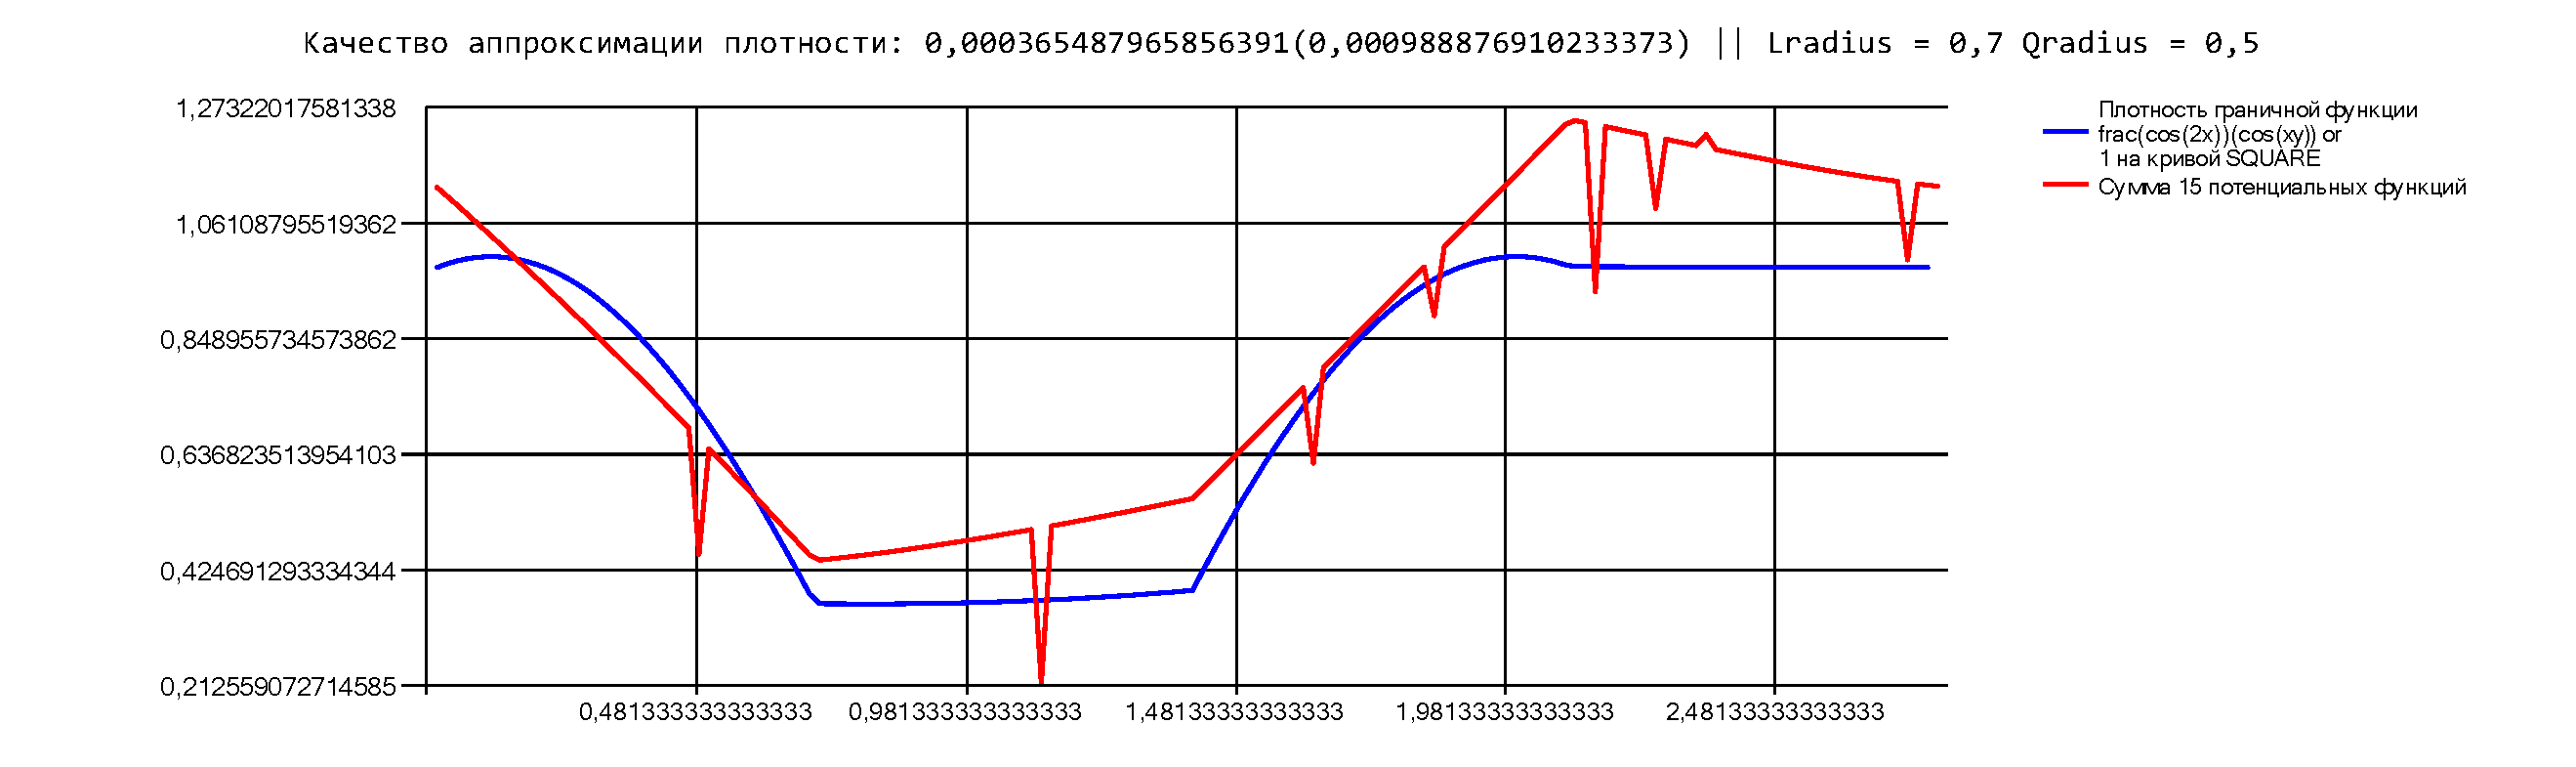
\includegraphics[width=0.8\linewidth]{d19.pdf} \\ для плотности} 
                        \end{minipage}} 
                        \vfill 
                        \center{\begin{minipage}[h]{\linewidth} 
                        \center{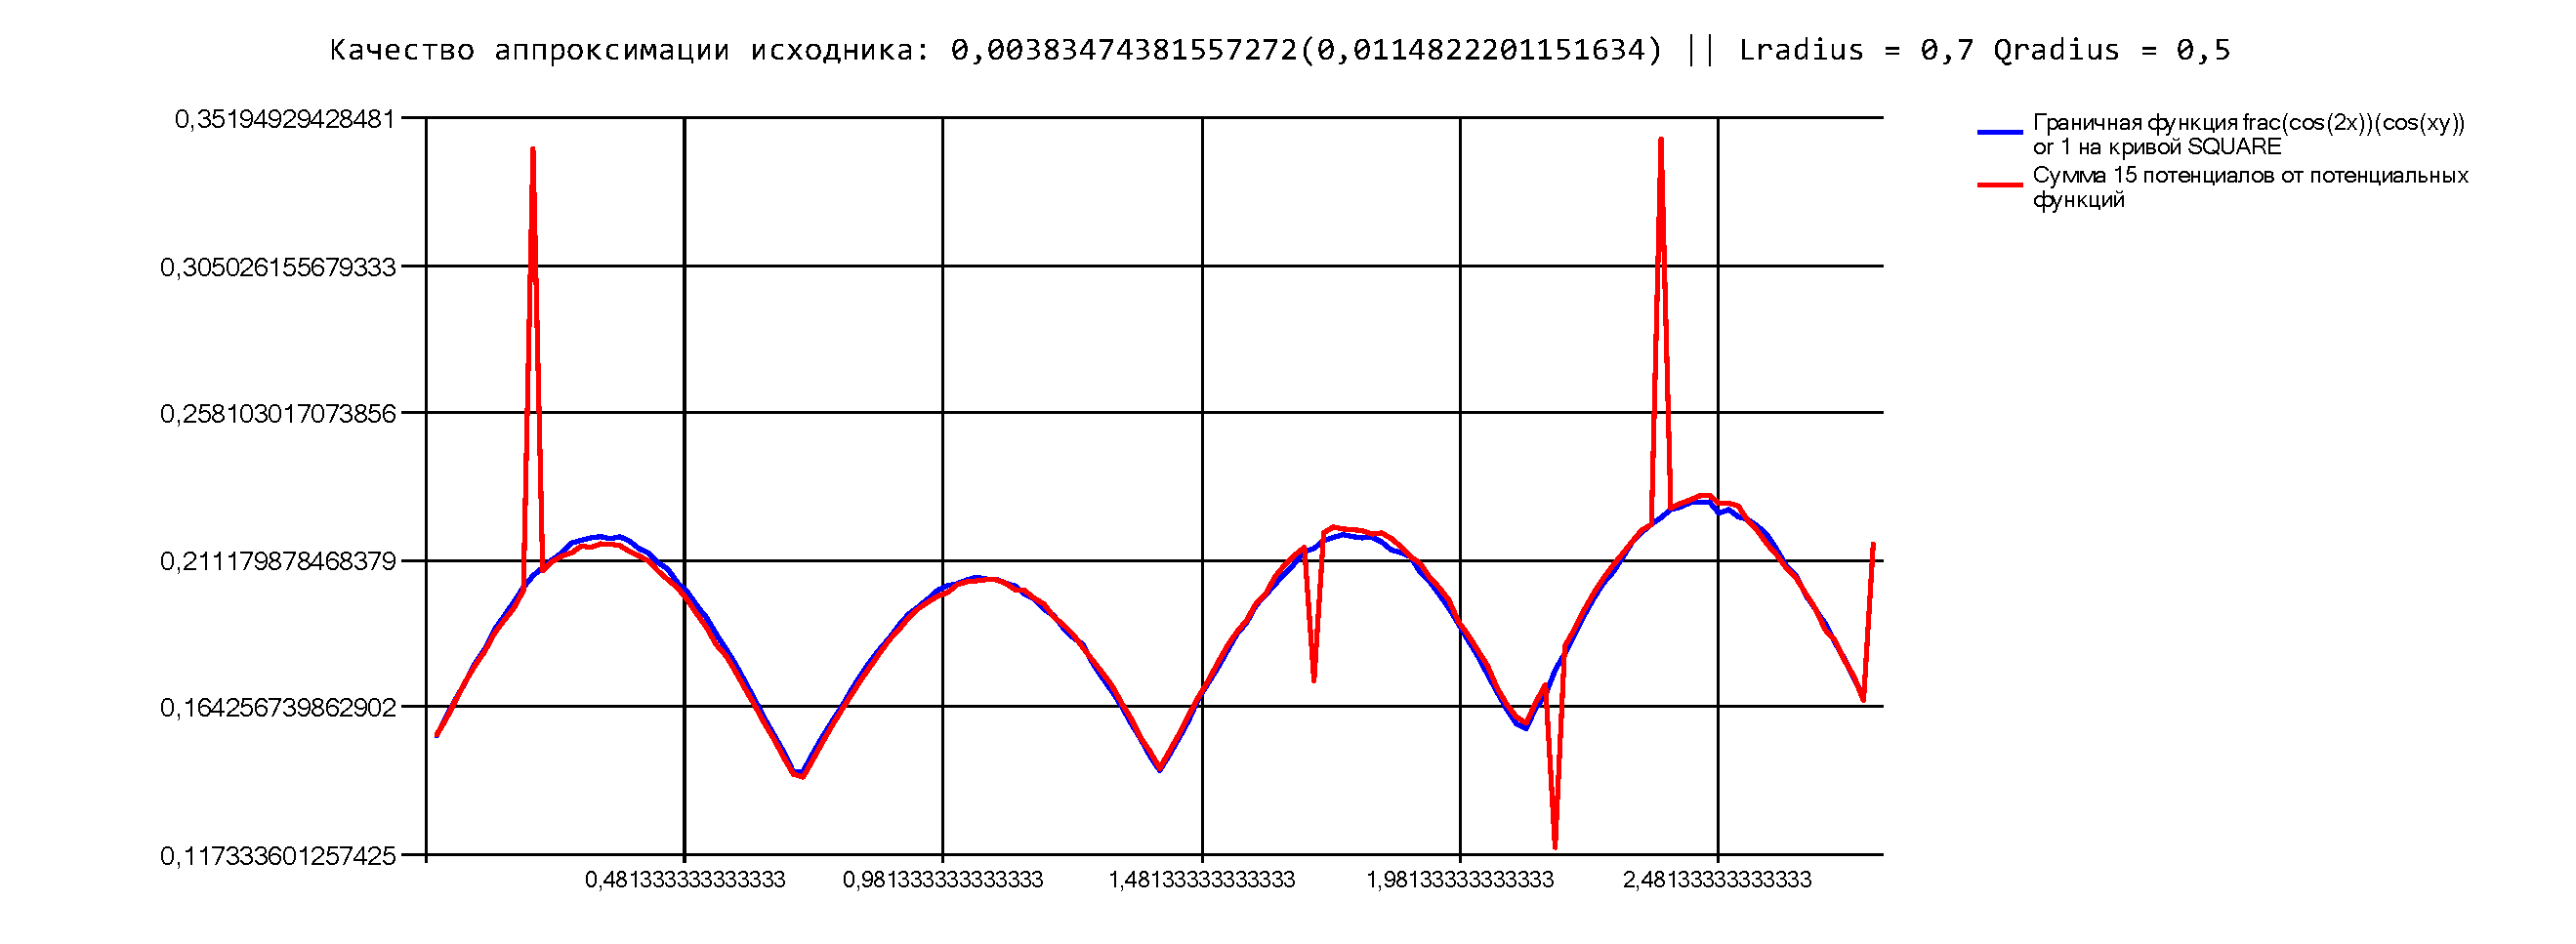
\includegraphics[width=0.8\linewidth]{v19.pdf} \\ для потенциала} 
                        \end{minipage}} 
                        \caption{Один из результатов работы алгоритма} 
                        \label{ris:image1} 
                        \end{figure}


                        \begin{figure}[h] 
                          \center{\begin{minipage}[h]{\linewidth} 
                          \center{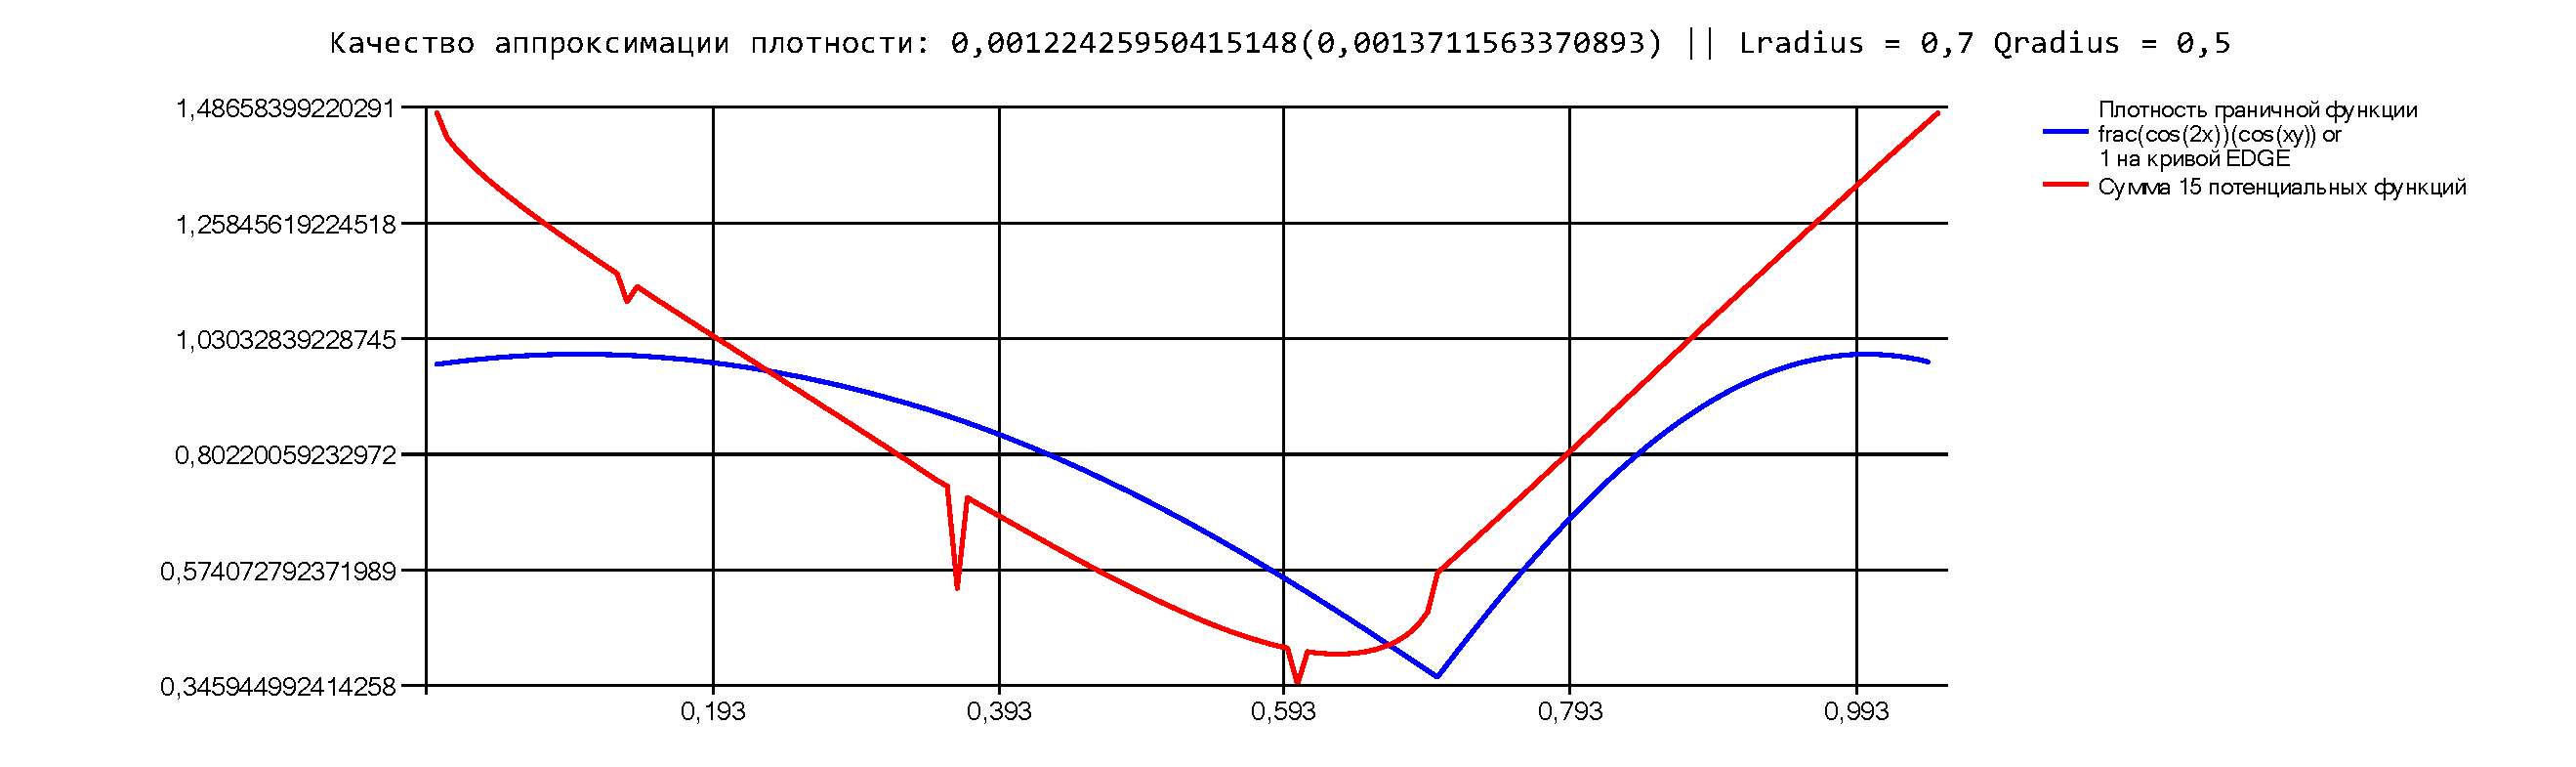
\includegraphics[width=0.8\linewidth]{d20.pdf} \\ для плотности} 
                          \end{minipage}} 
                          \vfill 
                          \center{\begin{minipage}[h]{\linewidth} 
                          \center{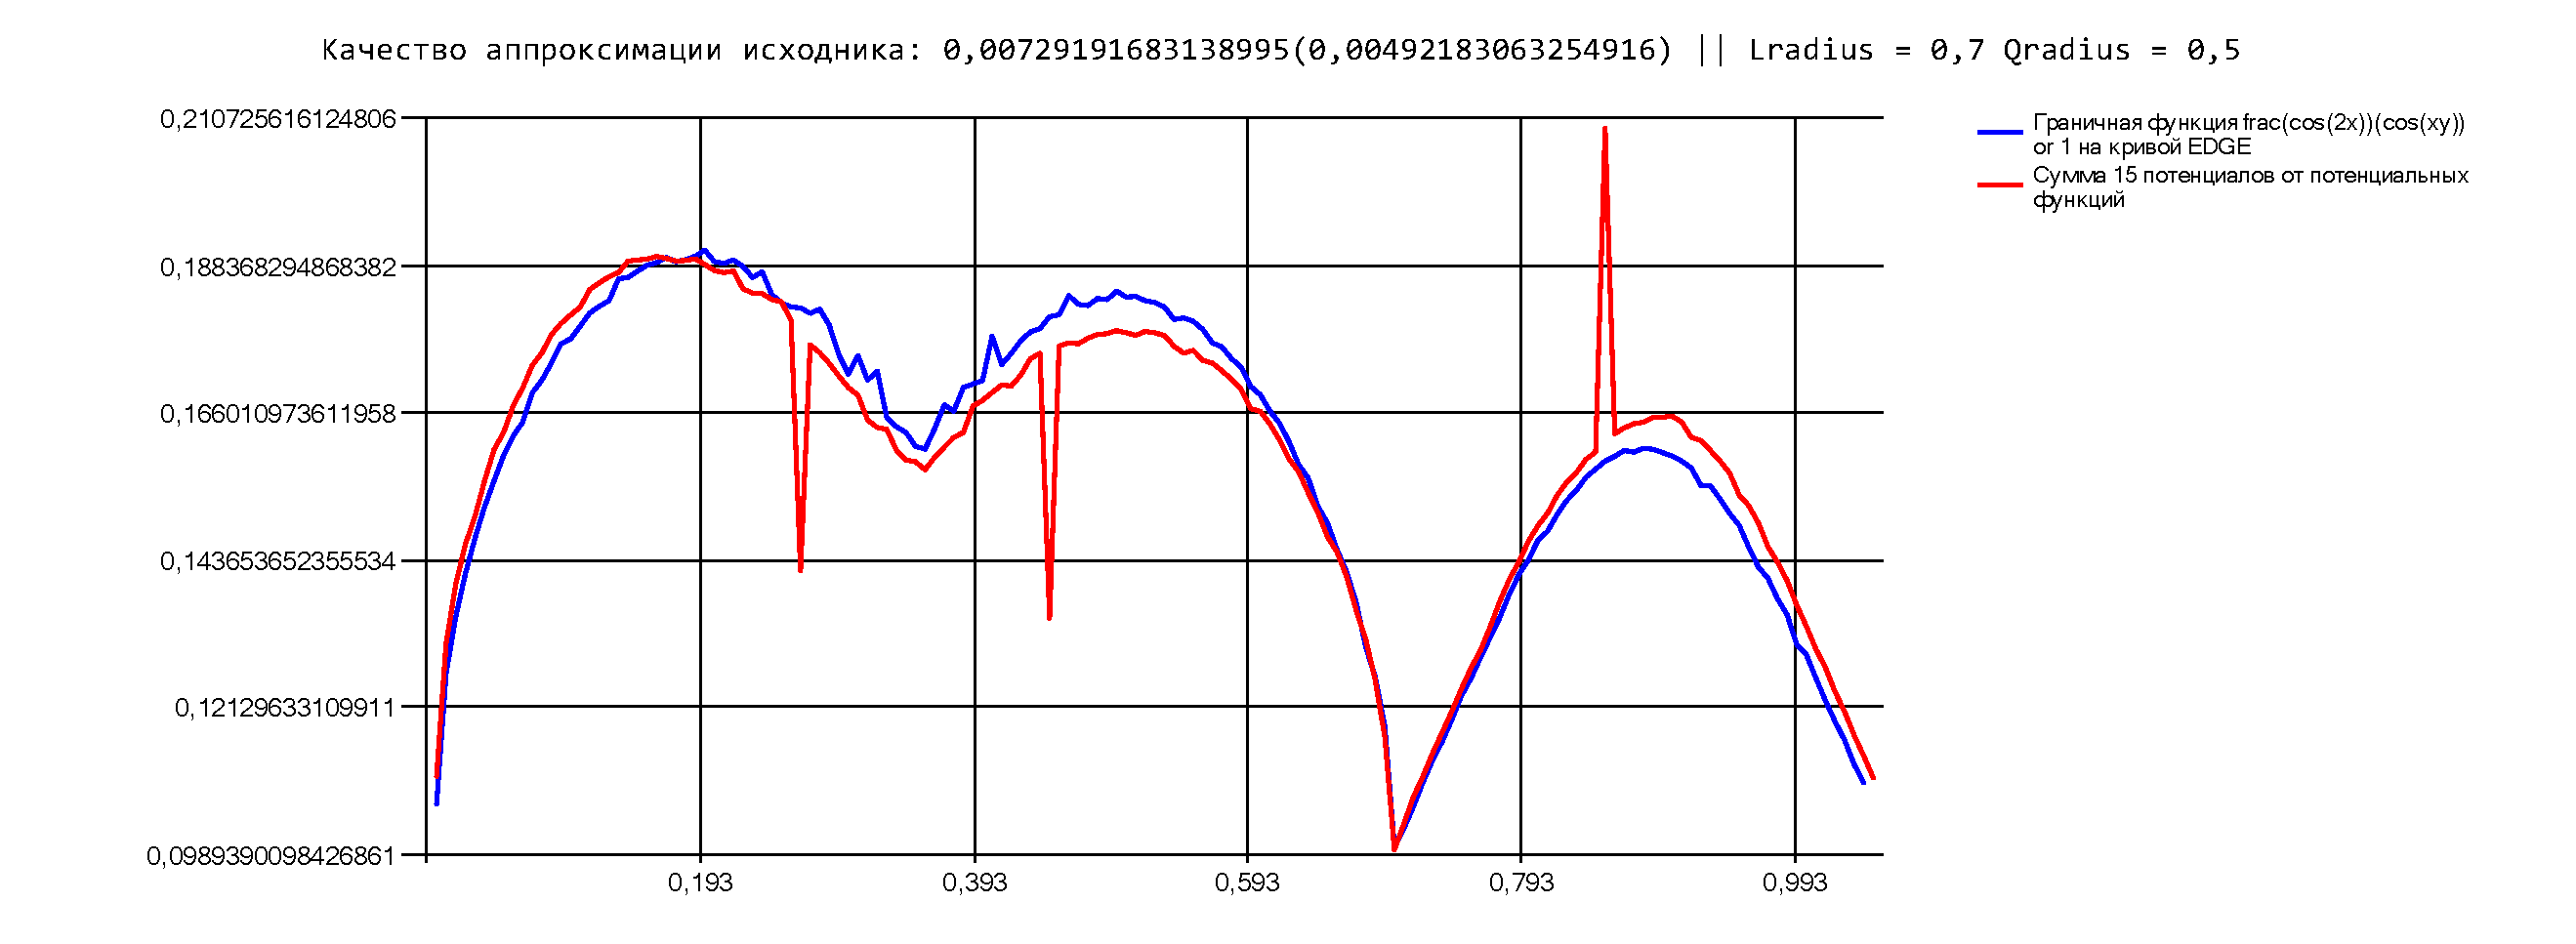
\includegraphics[width=0.8\linewidth]{v20.pdf} \\ для потенциала} 
                          \end{minipage}} 
                          \caption{Один из результатов работы алгоритма} 
                          \label{yyy} 
                          \end{figure}

                          \begin{figure}[h] 
                            \center{\begin{minipage}[h]{\linewidth} 
                            \center{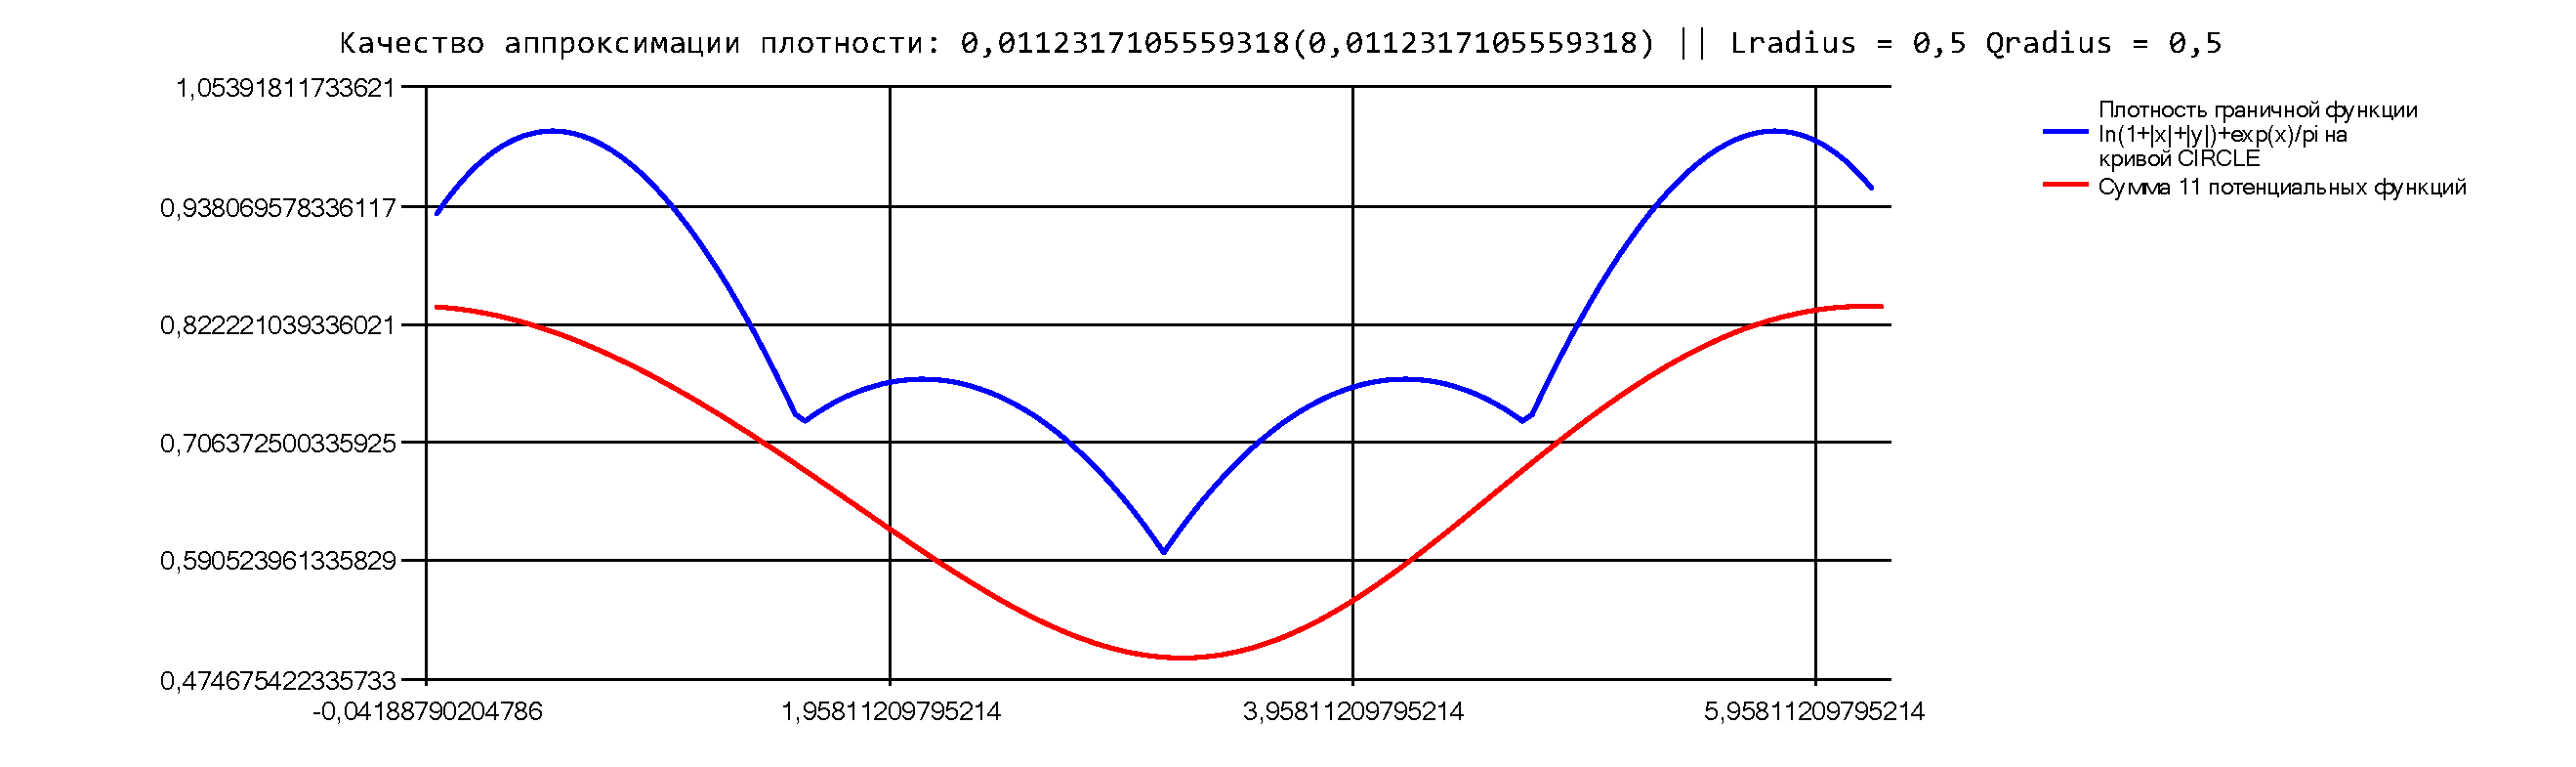
\includegraphics[width=0.8\linewidth]{d21.pdf} \\ для плотности} 
                            \end{minipage}} 
                            \vfill 
                            \center{\begin{minipage}[h]{\linewidth} 
                            \center{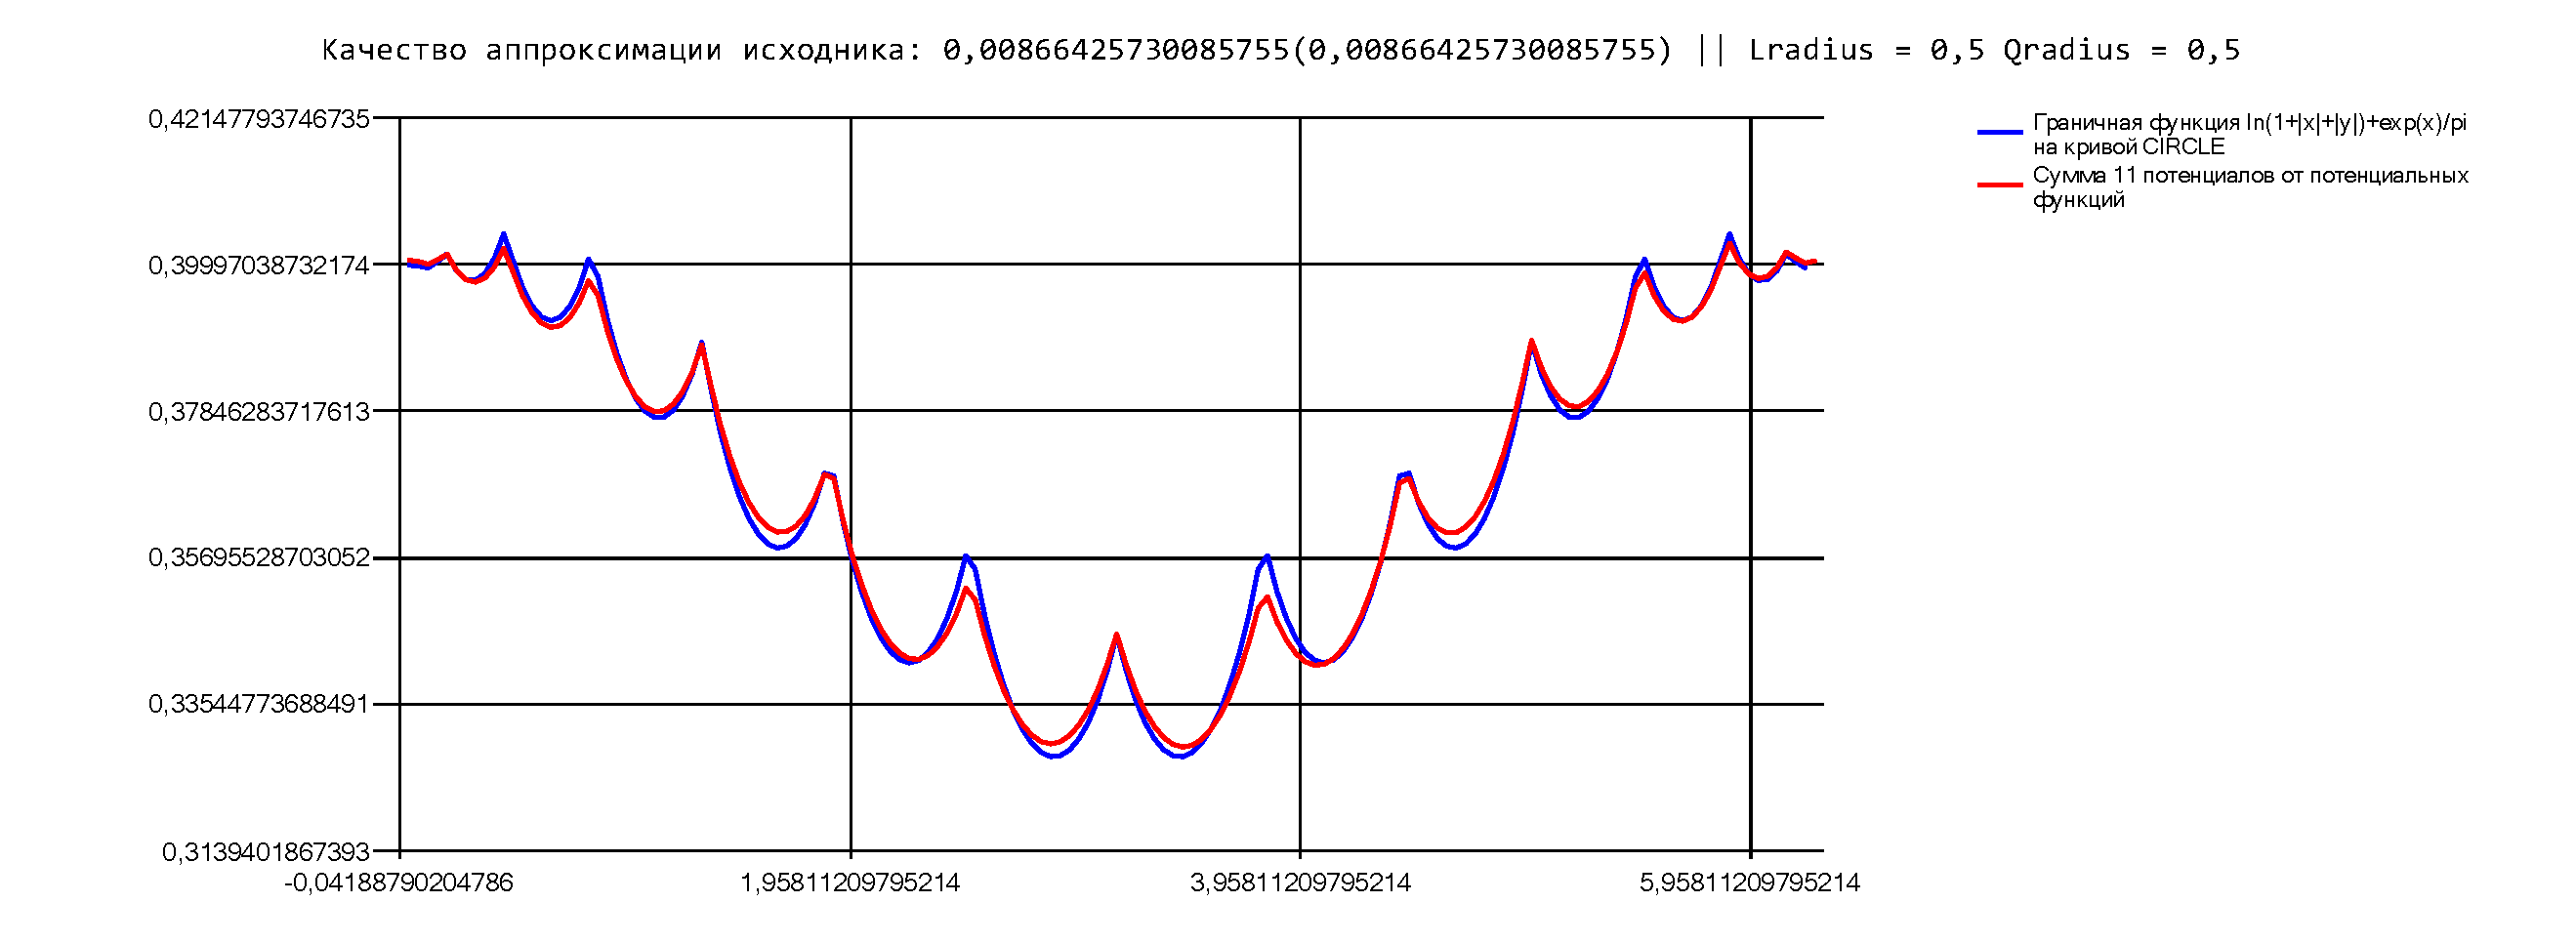
\includegraphics[width=0.8\linewidth]{v21.pdf} \\ для потенциала} 
                            \end{minipage}} 
                            \caption{Один из результатов работы алгоритма} 
                            \label{p6} 
                            \end{figure}

                            \begin{figure}[h] 
                              \center{\begin{minipage}[h]{\linewidth} 
                              \center{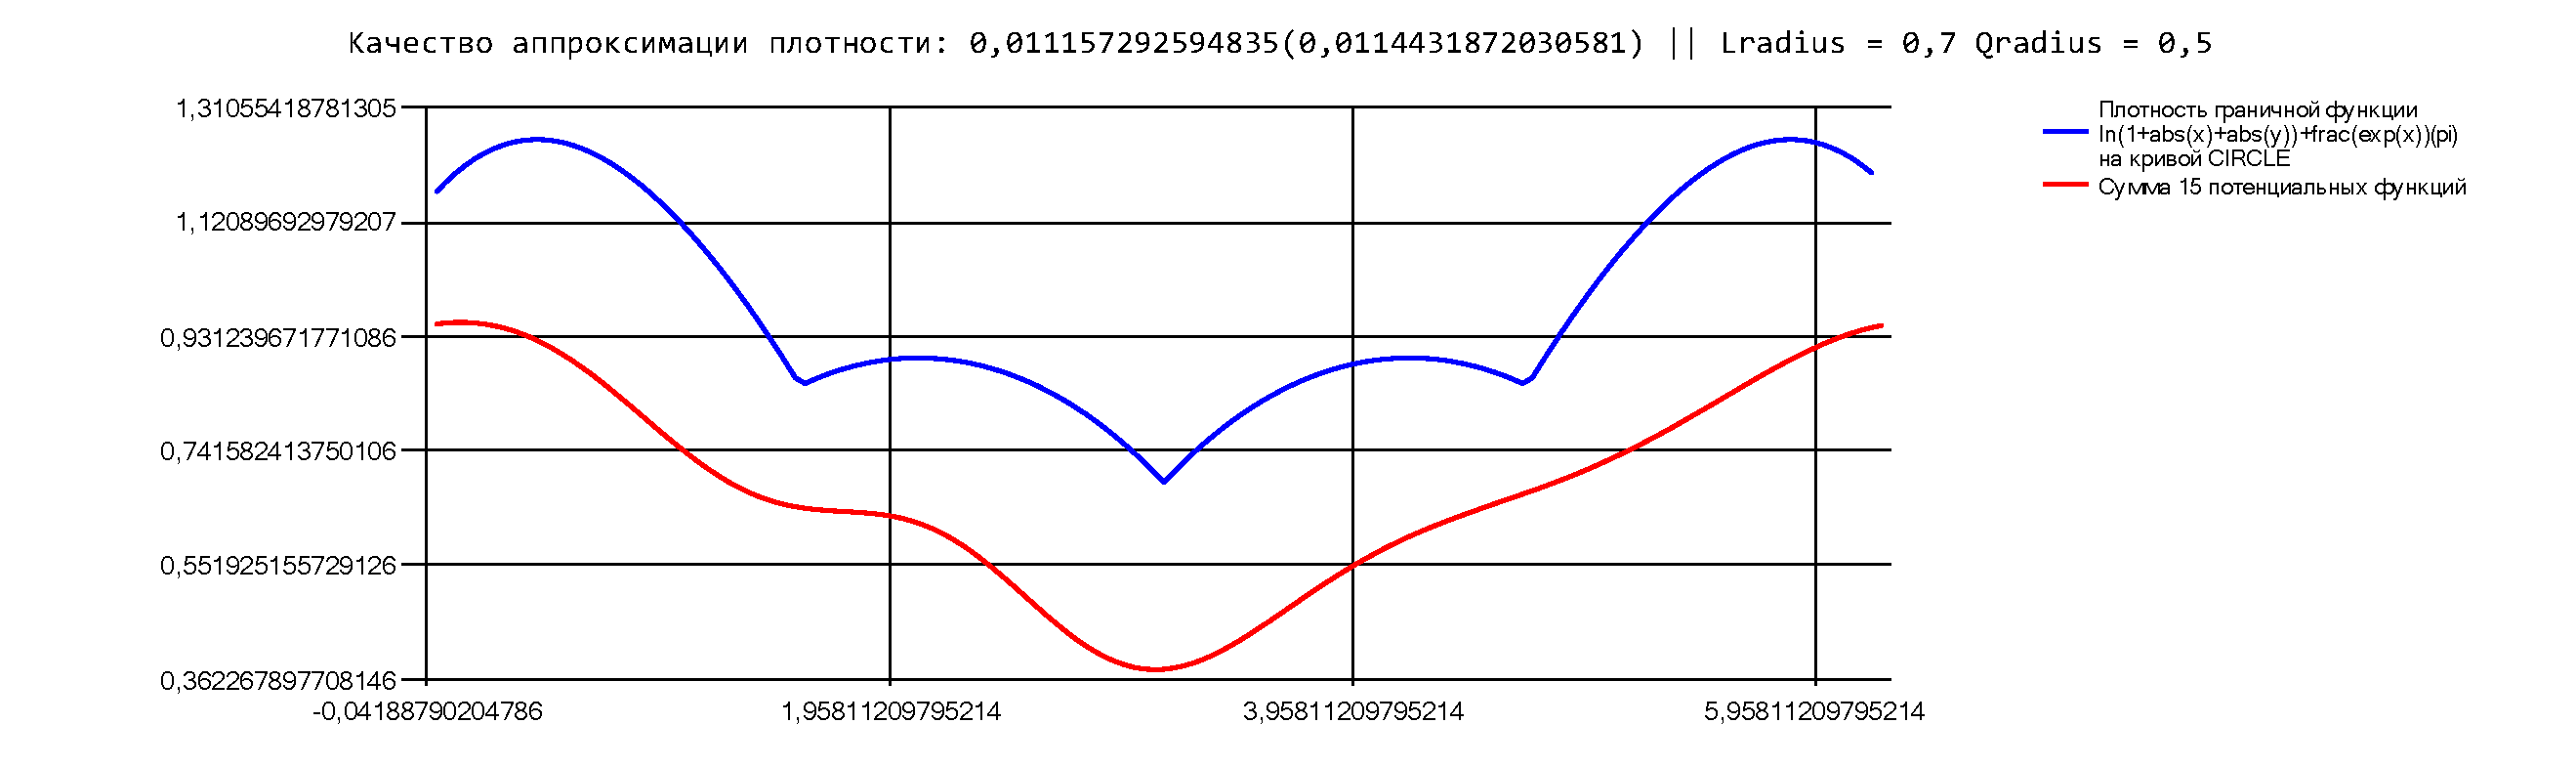
\includegraphics[width=0.8\linewidth]{d22.pdf} \\ для плотности} 
                              \end{minipage}} 
                              \vfill 
                              \center{\begin{minipage}[h]{\linewidth} 
                              \center{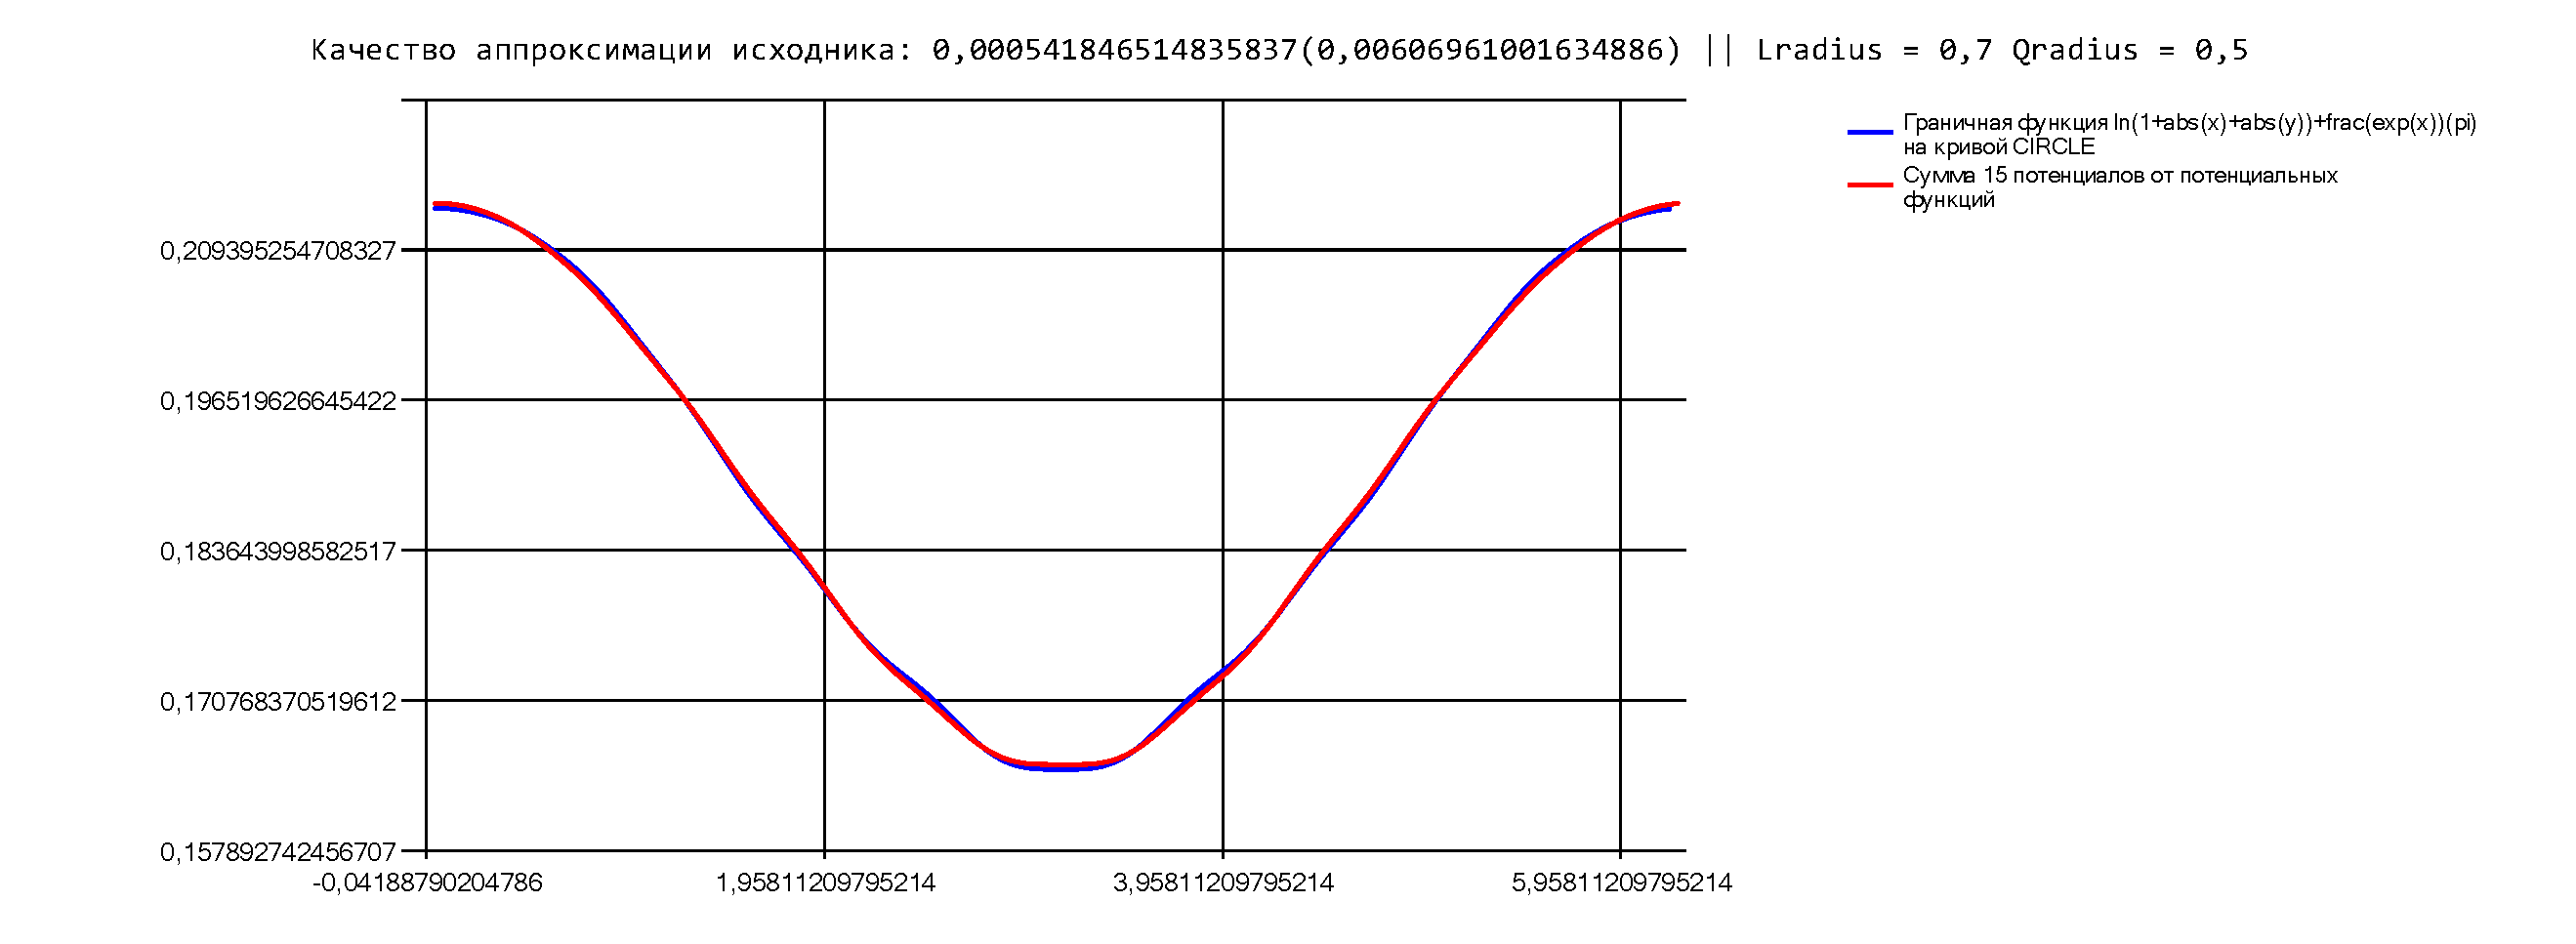
\includegraphics[width=0.8\linewidth]{v22.pdf} \\ для потенциала} 
                              \end{minipage}} 
                              \caption{Один из результатов работы алгоритма} 
                              \label{p7} 
                              \end{figure}


                              \begin{figure}[h] 
                                \center{\begin{minipage}[h]{\linewidth} 
                                \center{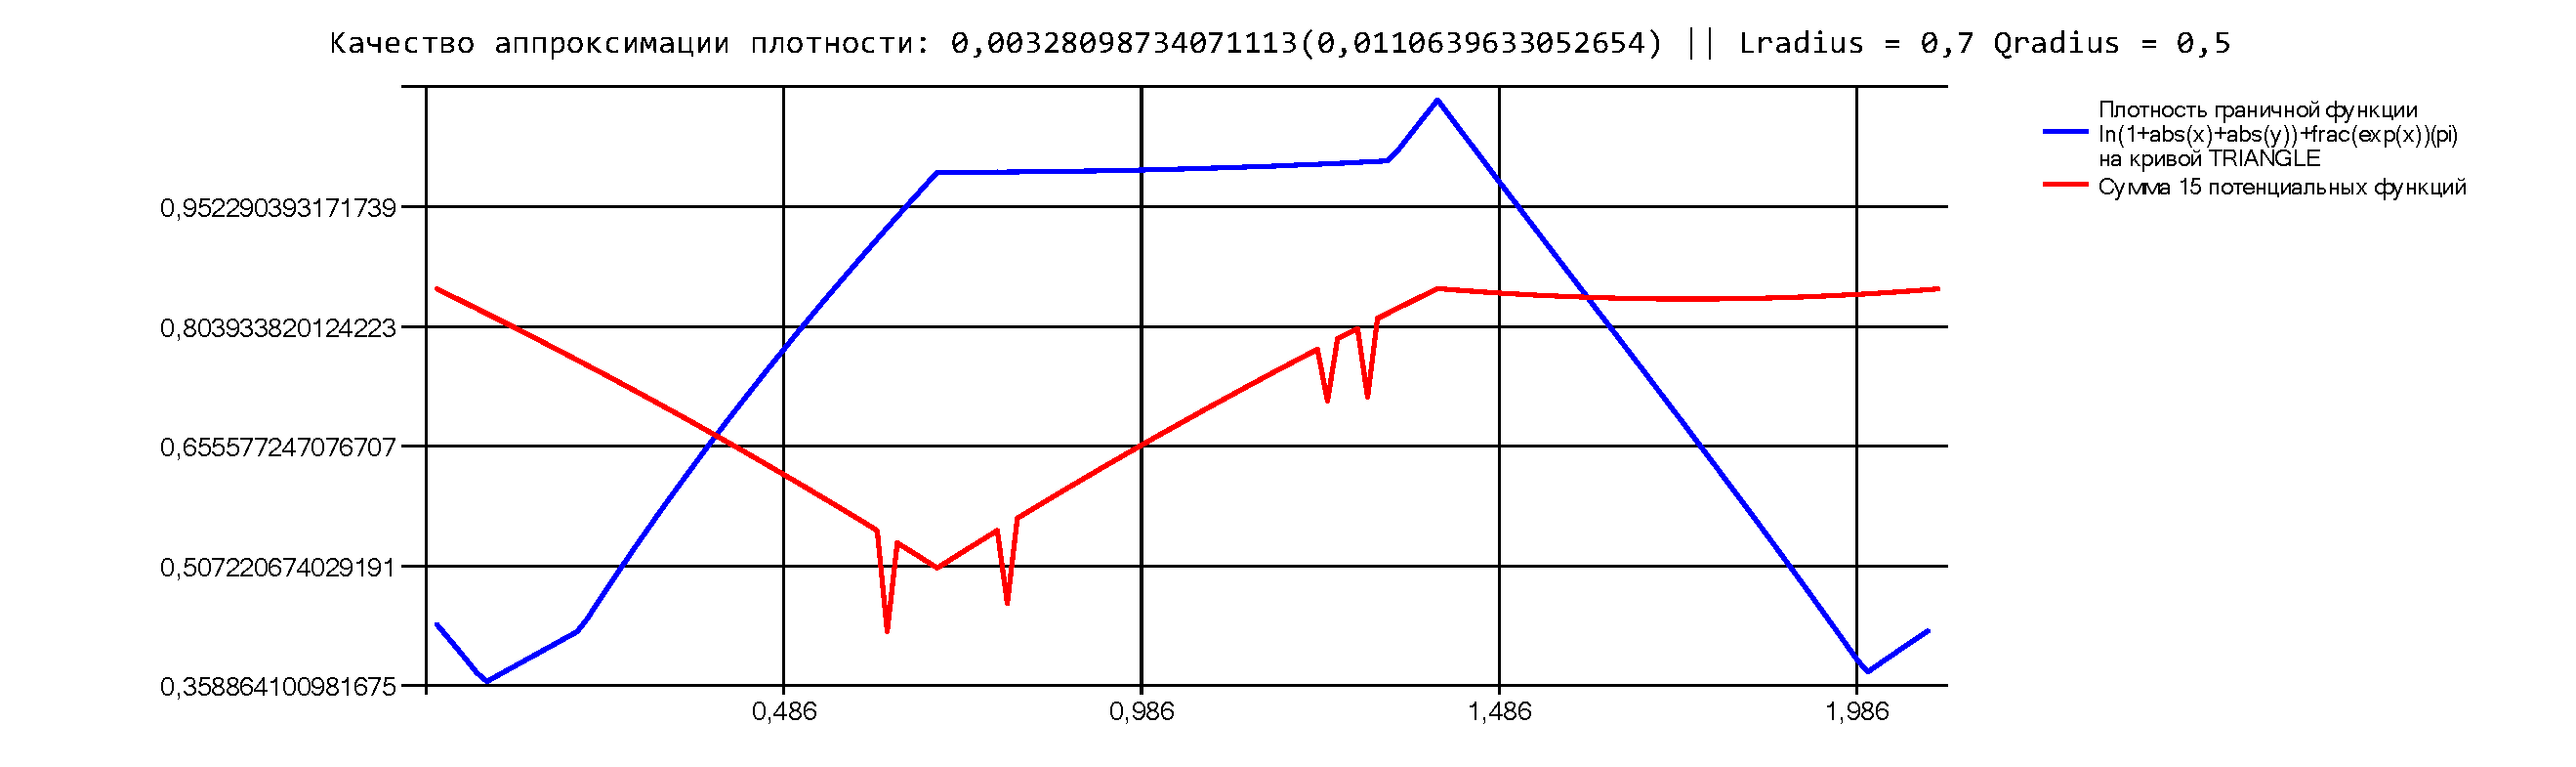
\includegraphics[width=0.8\linewidth]{d23.pdf} \\ для плотности} 
                                \end{minipage}} 
                                \vfill 
                                \center{\begin{minipage}[h]{\linewidth} 
                                \center{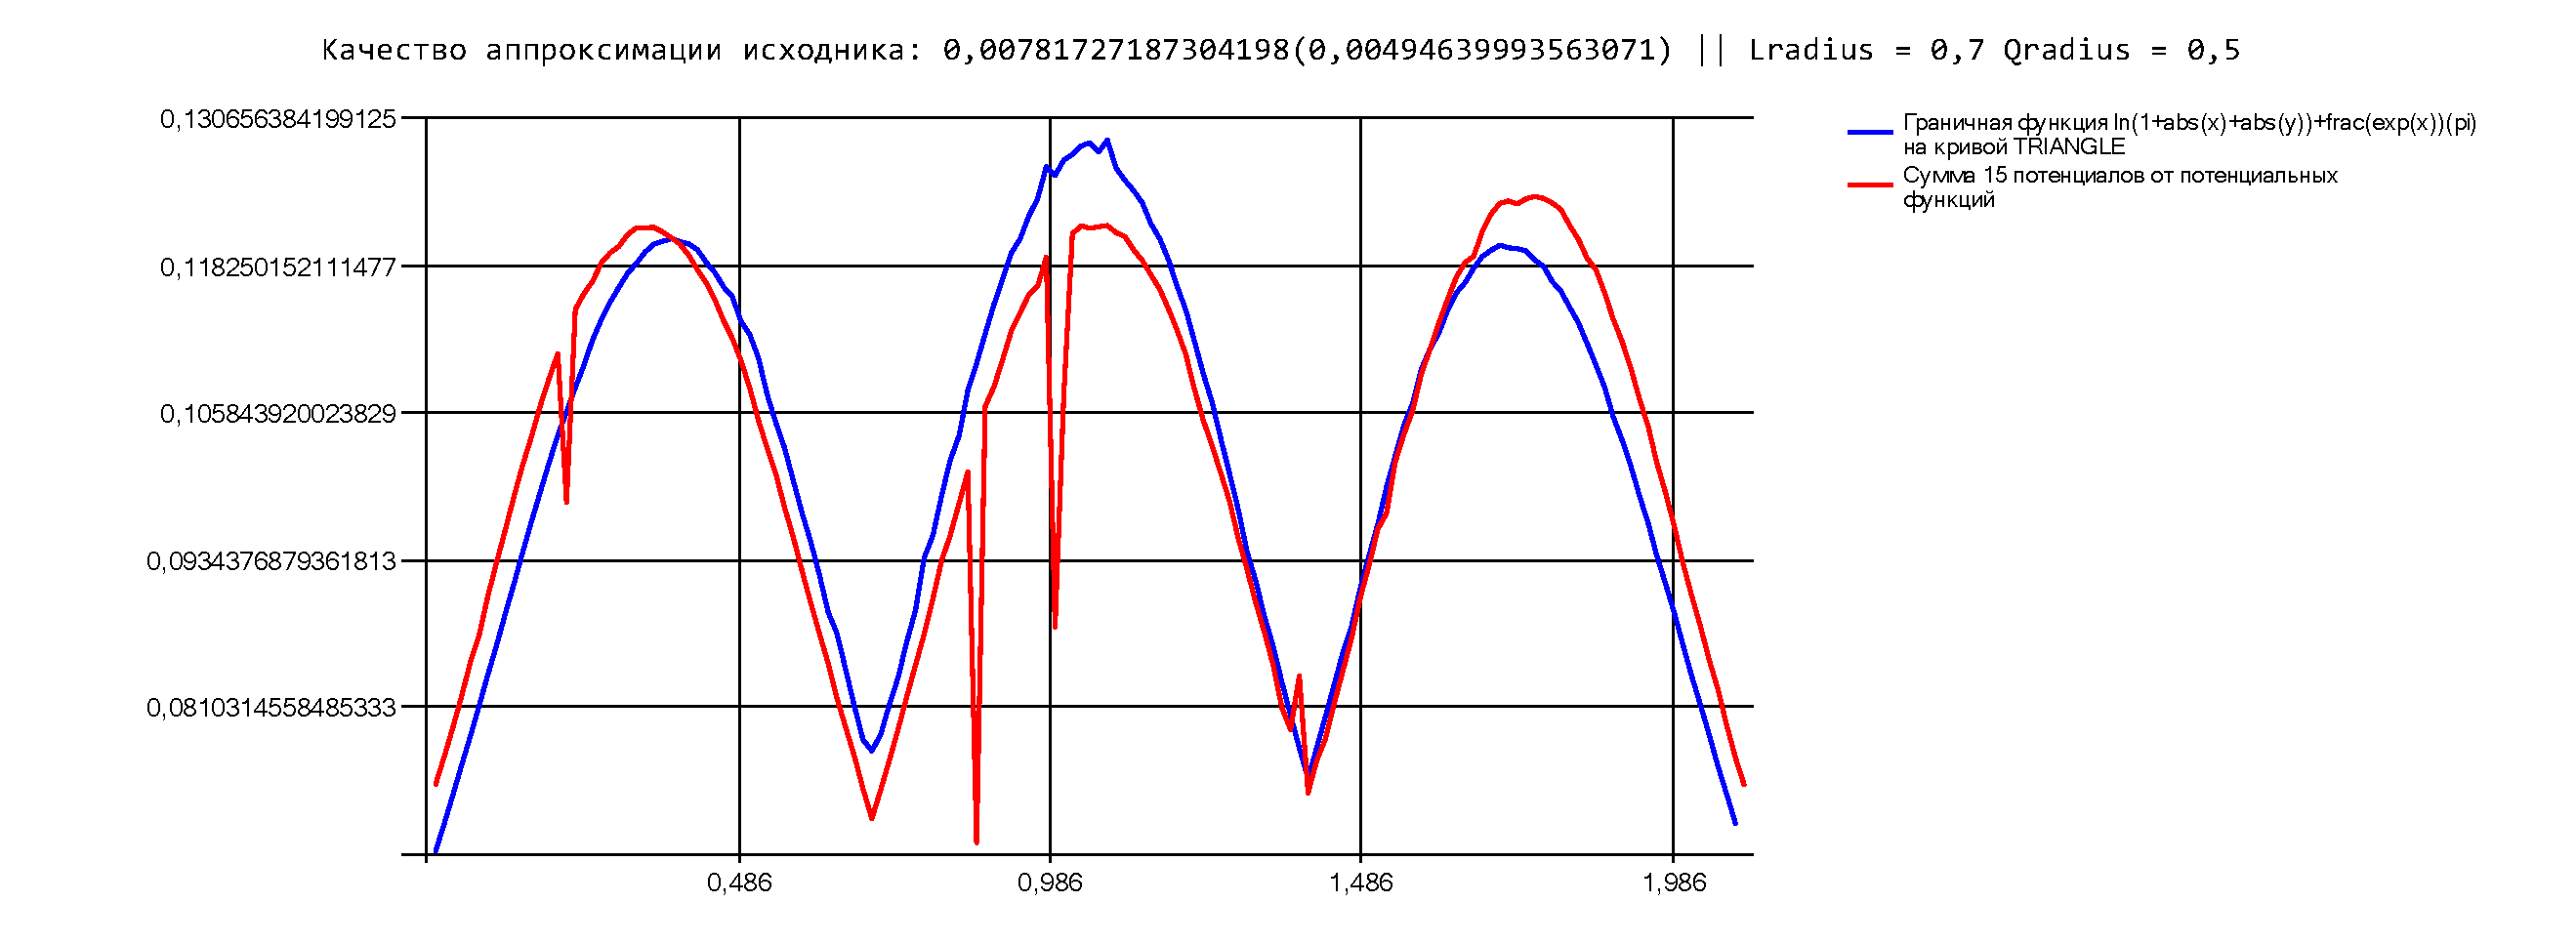
\includegraphics[width=0.8\linewidth]{v23.pdf} \\ для потенциала} 
                                \end{minipage}} 
                                \caption{Один из результатов работы алгоритма} 
                                \label{ris:image1} 
                                \end{figure}                                          


                                \begin{figure}[h] 
                                  \center{\begin{minipage}[h]{\linewidth} 
                                  \center{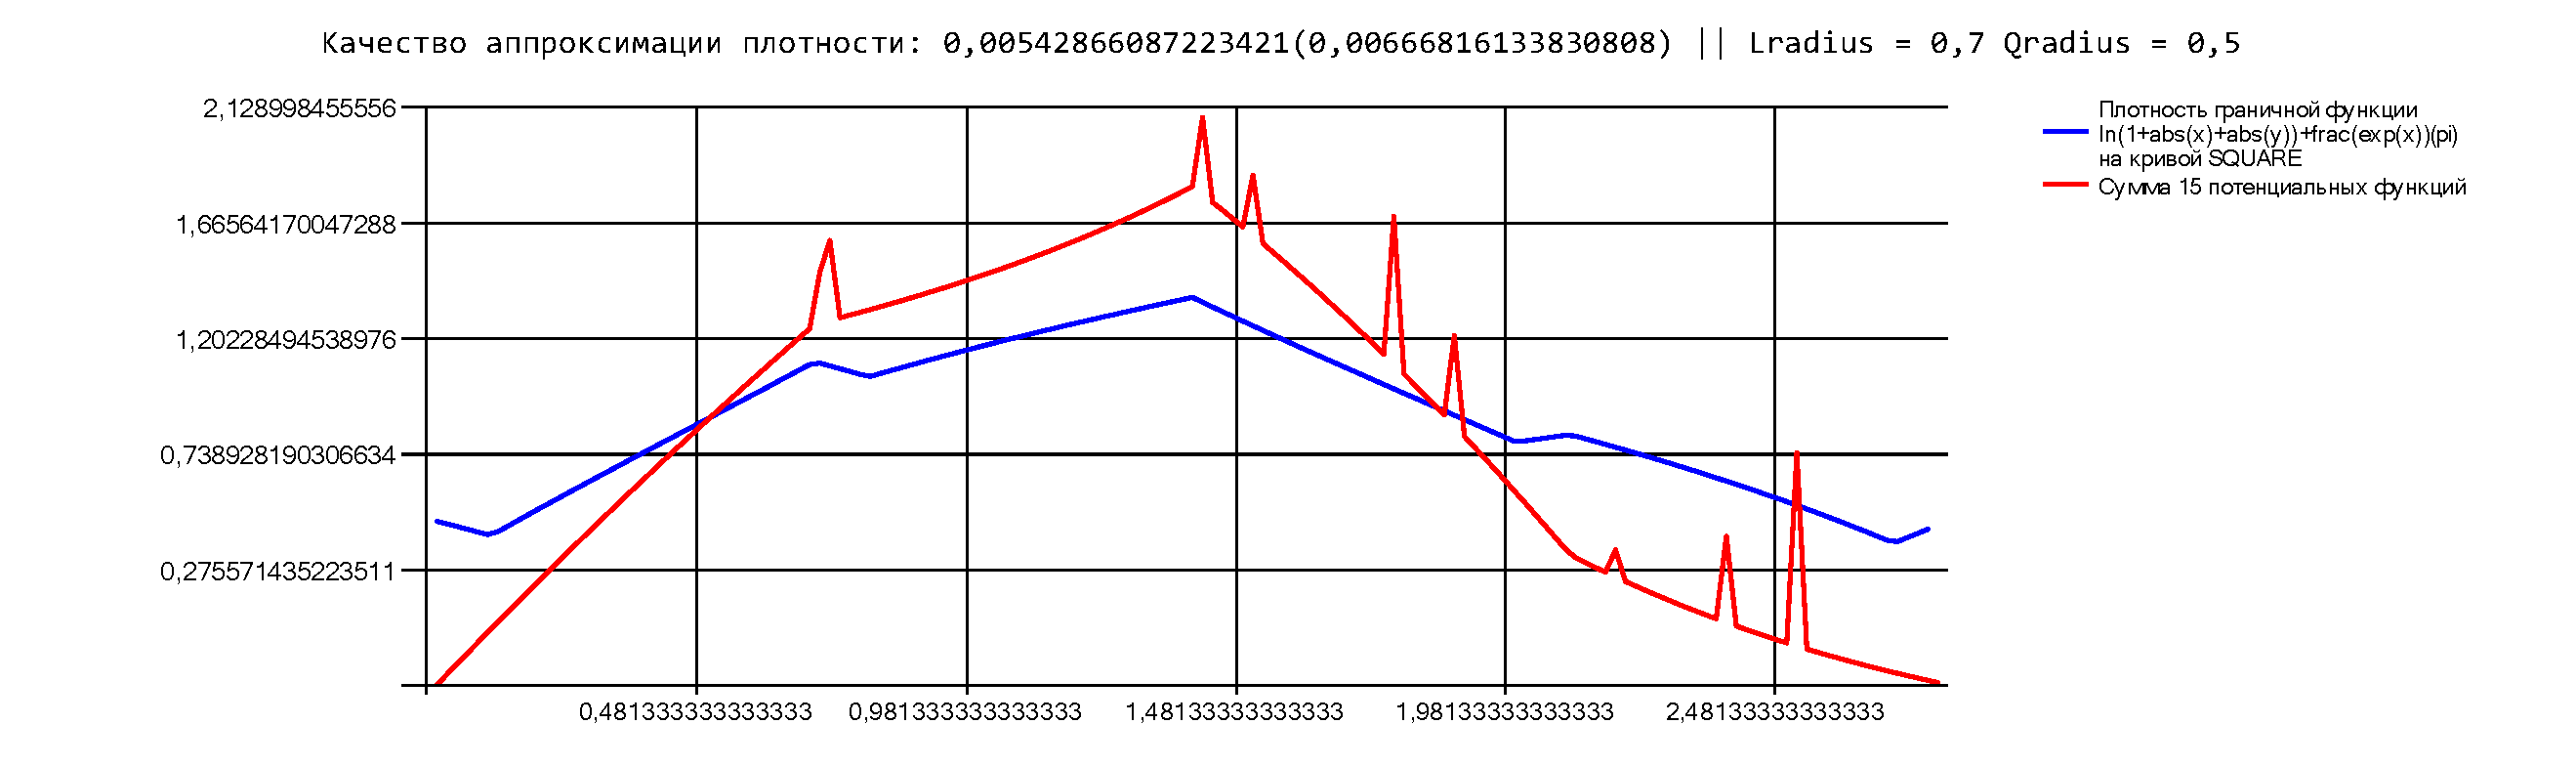
\includegraphics[width=0.8\linewidth]{d24.pdf} \\ для плотности} 
                                  \end{minipage}} 
                                  \vfill 
                                  \center{\begin{minipage}[h]{\linewidth} 
                                  \center{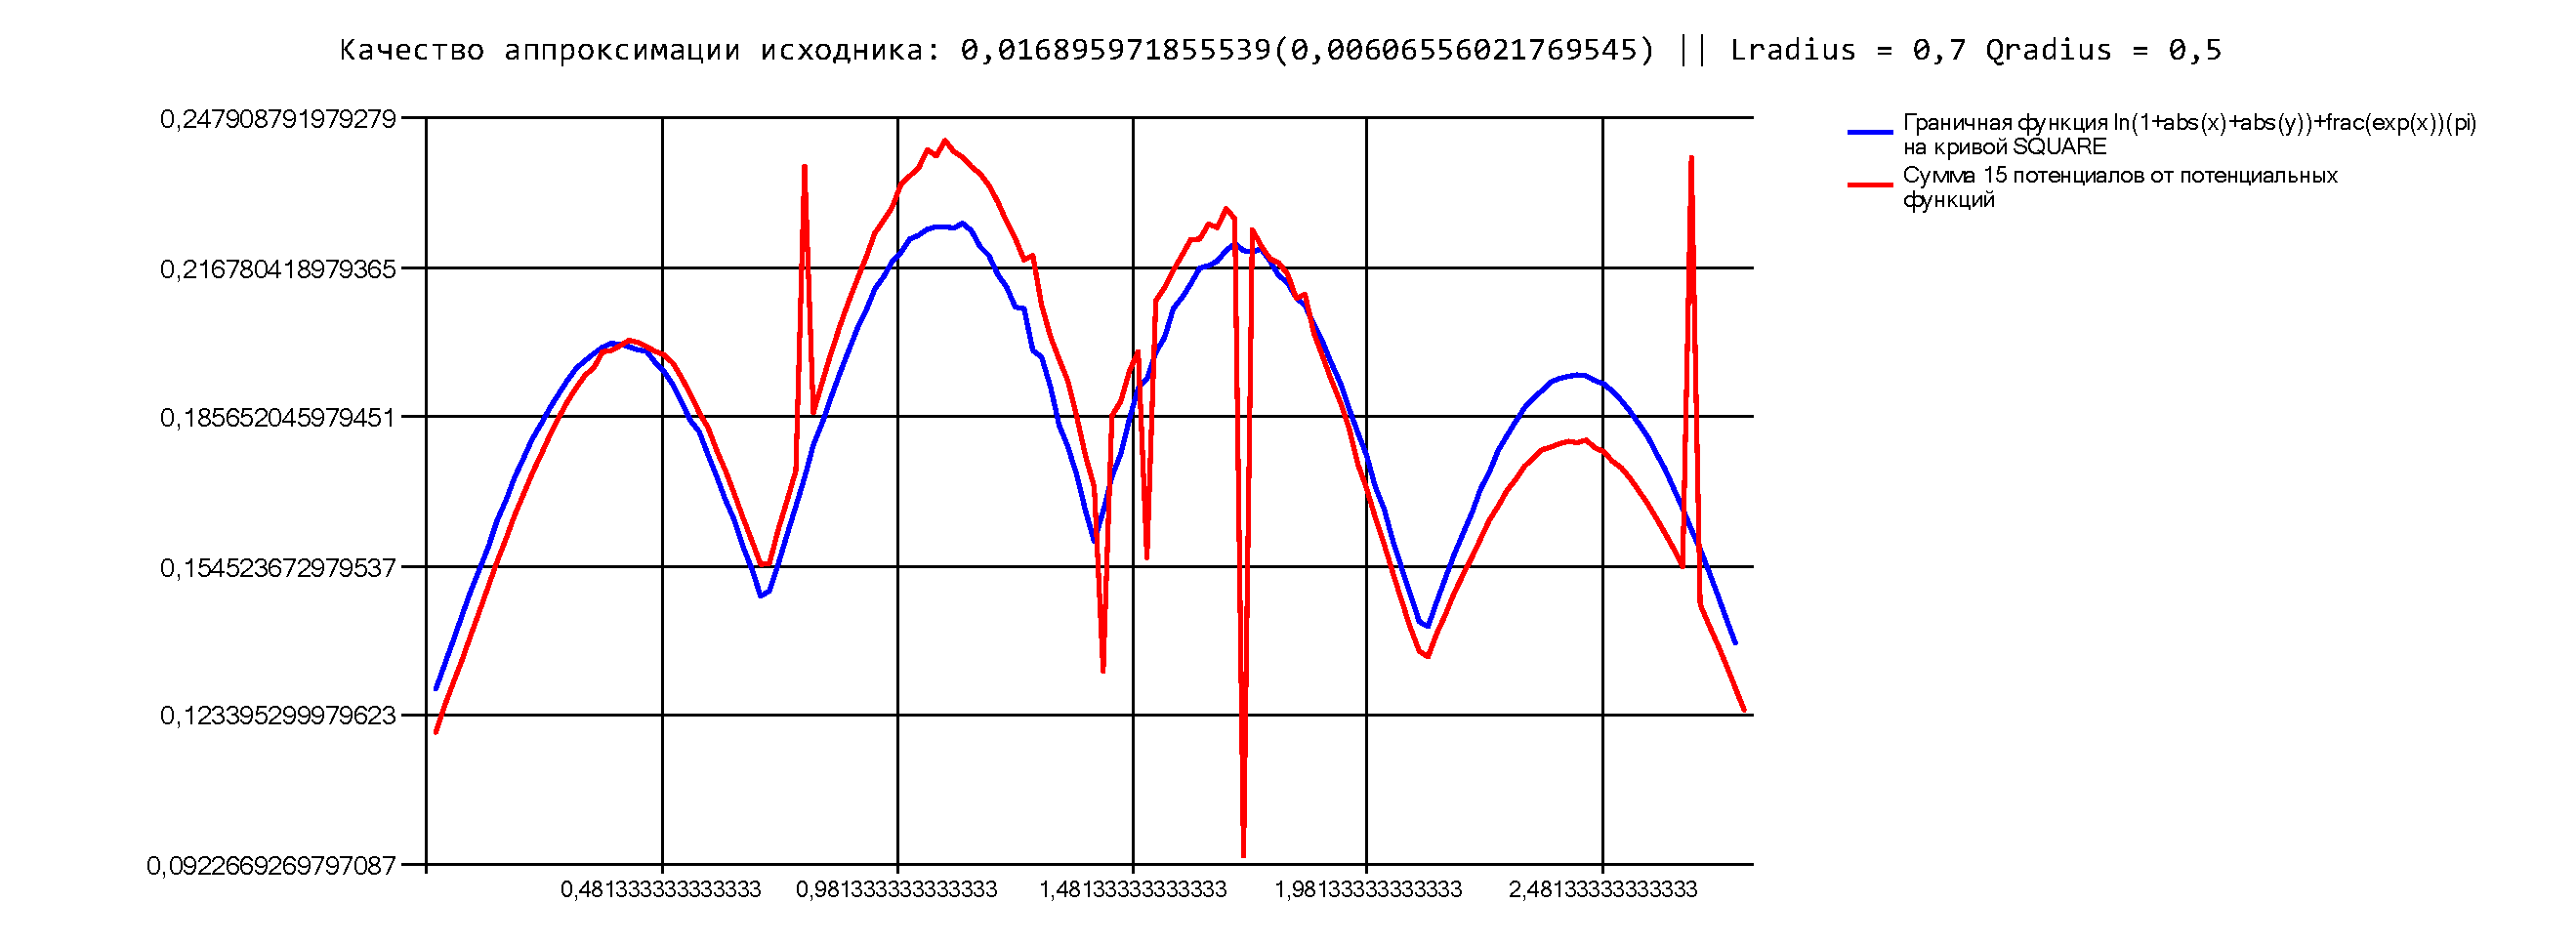
\includegraphics[width=0.8\linewidth]{v24.pdf} \\ для потенциала} 
                                  \end{minipage}} 
                                  \caption{Один из результатов работы алгоритма} 
                                  \label{gend} 
                                  \end{figure}        

\section*{\appendixname\ A. Пример построения параметризации вложенных кривых}
Пусть требуется провести интегрирование по полукругу из верхней полуплоскости (рисунок \ref{hcircapp}) описанным ранее методом.
Для этого требуется задать такую параметризацию полукруга в зависимости от параметра $r$, чтобы с уменьшением $r$ получались вложенные друг в друга кривые, подобные границе полукруга.
\begin{figure}[h!]
  \noindent\centering{
  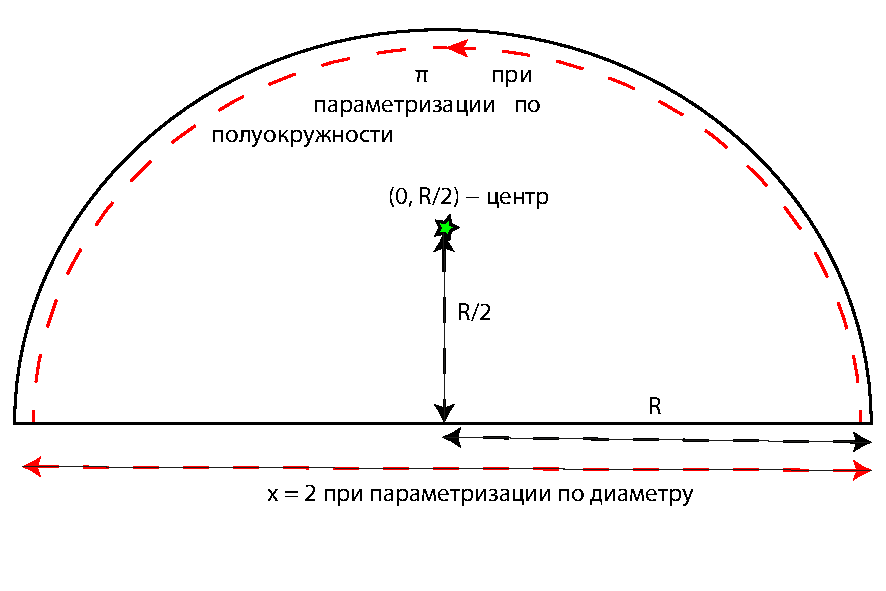
\includegraphics[width=\linewidth]{halfcirc.pdf}
}
  \caption{Полукруг радиуса $R$ c центром в $(0, \frac{R}{2})$}
  \label{hcircapp}
  \end{figure} 
В общем случае требуется проделать следующие действия:
\begin{enumerate}
  \item  {\itОпределить центр области}. Под центр области можно взять любую точку внутри области, лишь бы потом было легко задать такую параметризацию, чтобы при уменьшении $r$ происходило сужение в какую-то точку внутри области.
  В качестве центра можно взять и вообще произвольную точку, но тогда задавать параметризацию будет труднее. В данном случае вполне естественным будет задать центр в точке $(0,\frac{R}{2})$.
  \item {\itОпределение радиуса $r$ (что именно брать за радиус)}. В данном случае под радиусом $r$ естественно взять радиус полуокружности.
  \item {\itОпределение отрезка параметризации}. Отрезок параметризации можно выбрать любым, лишь бы при интегрировании по нему точки, в которых считается интеграл, располагались равномерно; при этом для равномерного расположения точек по области нужно, чтобы длина отрезка параметризации была постоянной (не зависела от радиуса); если же нужно сгущение точек в каких-то местах, это учитывается на этапе задания отрезка. В нашем случае длина полуокружности равна $\pi R$, длина диаметра --- $2R$. Тогда, если для параметризации полуокружности взять отрезок длины $\pi$, для параметризации диаметра придётся взять отрезок длины $x$ такой, что $\frac{\pi R}{2R}=\frac{\pi}{x} \Rightarrow x=2$.
  \item {\itЗадание параметризации границы интегрируемой области}. В нашем случае можно взять такую параметризацию:
  \begin{equation}
    {\bf r}(t)=
    \begin{cases}
      \begin{pmatrix}
        R \cos(t)\\
        R \sin(t)
      \end{pmatrix}, & t \in [0,\pi]\\
    \begin{pmatrix}
      -R+(t-\pi)R\\
      0
    \end{pmatrix}, & t \in [\pi,\pi+2]
  \end{cases}
  \end{equation}.
  \item {\itЗадание параметризации подобных кривых}. Если знать параметризацию границы, для задания параметризации подобных кривых потребуется лишь заменить $R$ на параметр $r$ и учесть смещение координат. В нашем случае внутренние кривые (изображены на рисунке \ref{hcircp}) будут иметь параметризацию
  \begin{equation}
    {\bf r}(t,r)=
    \begin{cases}
      \begin{pmatrix}
        r \cos(t)\\
        r \sin(t)+ \frac{1}{2}(R-r)
      \end{pmatrix}, & t \in [0,\pi]\\
    \begin{pmatrix}
      -r+(t-\pi)r\\
      \frac{1}{2}(R-r)
    \end{pmatrix}, & t \in [\pi,\pi+2]
  \end{cases}
  \end{equation}.
  \begin{figure}[h!]
    \noindent\centering{
    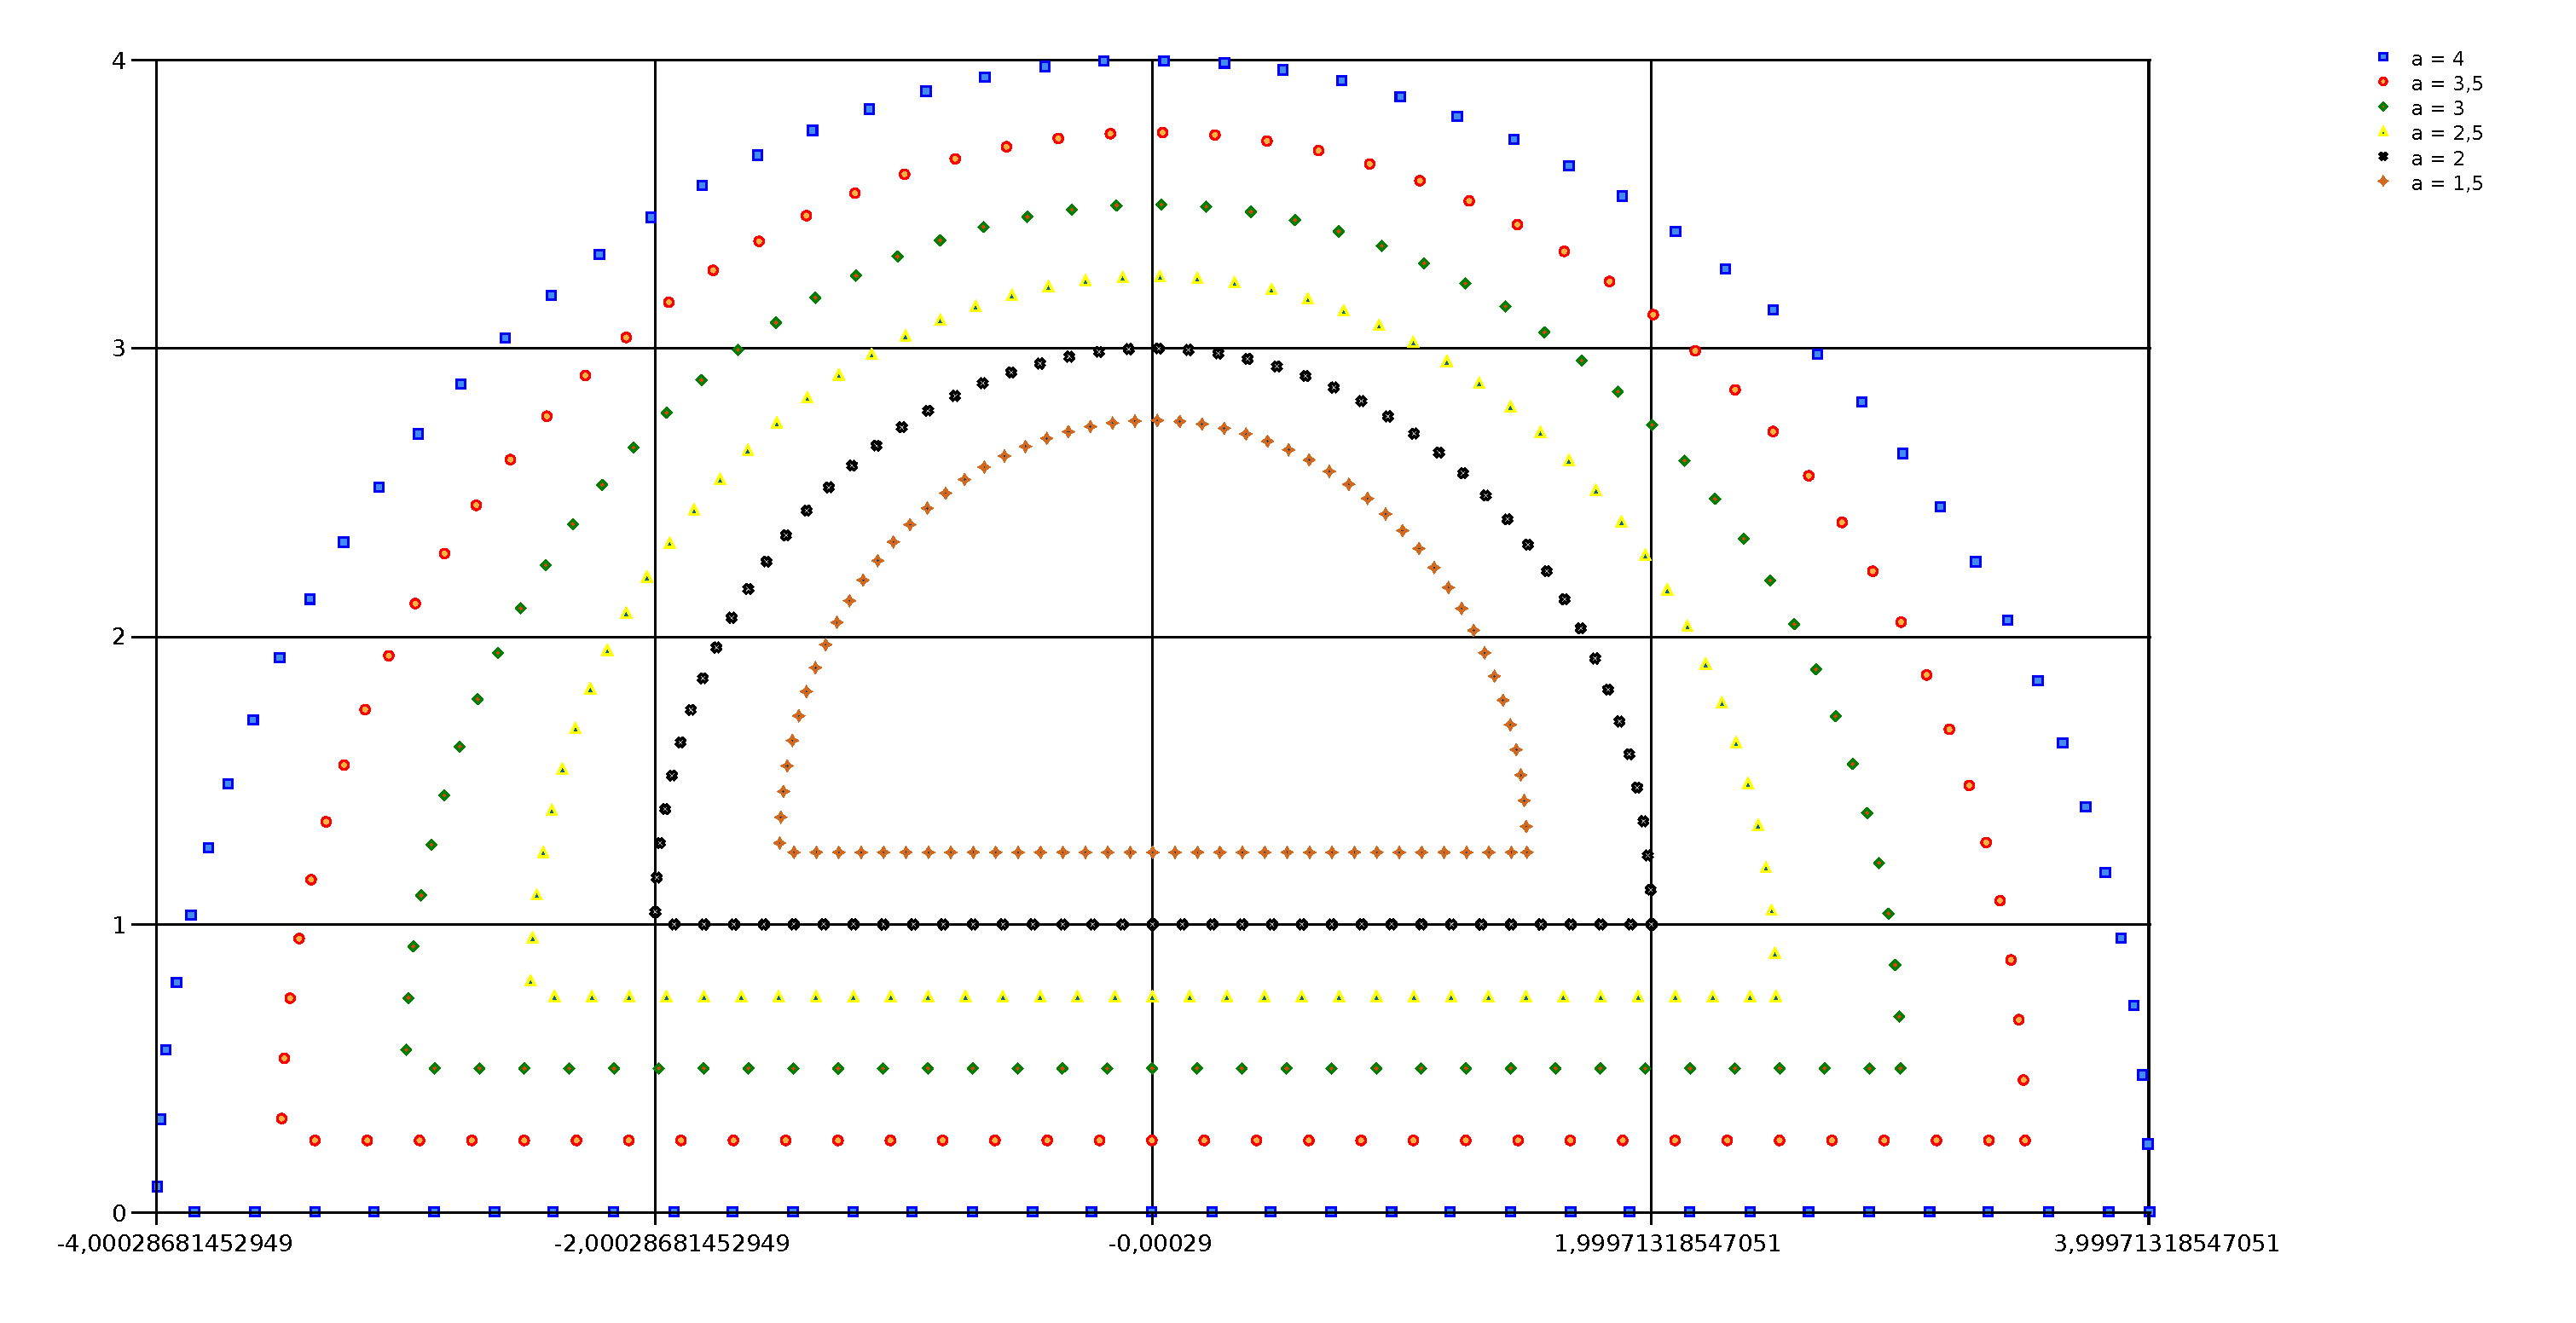
\includegraphics[width=\linewidth]{hcircp.pdf}
  }
    \caption{Вложенные полукруги. Обратите внимание на приблизительно равномерное расположение точек}
    \label{hcircp}
    \end{figure}
    
    \item {\itОпределить площадь кольцевого сегмента}. Площадь сегмента $S=S(t_x,t_y,r)$, где $t_x$ --- шаг по отрезку параметризации, $t_y$ --- шаг по радиусу, $r$ --- радиус кривой в центре кольца (по которой и ведётся интегрирование), можно вычислить так. Сначала вычисляется площадь всего кольца как разность площадей двух областей (минимальной подобной области, содержащей кольцо, и максимальной подобной области, не содержащей кольцо): $\frac{1}{2} \pi (r+\frac{t_y}{2})^2-\frac{1}{2} \pi (r-\frac{t_y}{2})^2=\pi r t_y$; затем это выражение надо умножить на соотношение $\frac{t_x}{\pi +2}$ (шаг по отрезку параметризации на длину отрезка параметризации). В итоге получаем $S = \frac{t_x \pi r t_y}{\pi +2}$.

\end{enumerate}

\section{Вспомогательные утверждения}
В этом разделе доказываются некоторые утверждения, связанные со свойствами объемного потенциала и условиями однозначной разрешимости ОЗГ, накладываемыми на поверхность $S$.
\subsection{Объёмный потенциал и его свойства}

Пусть
$$V_{\rho}(x) \equiv \int_Q \rho(y) E(x-y) dy,$$
$Q$ --- ограниченная область в $\R{2}, x,y \ \in \R{2}, E(x)= -2 \pi \ln|x|, \rho \in L_2(Q)$.

\begin{Lem}
  $\forall x \in \R{2}$ интеграл $V_{\rho}(x)$ сходится в смысле Лебега.
\end{Lem}
\begin{Proof}
  Докажем, что $\forall x \in \R{2}$ функция $E(x-*) \in L_2(Q)$. Достаточно доказать, что $\int_Q E^2 (x-y) dy < +\infty$.
  
  $\exists R>0: Q \subset B_R(x)$ -- шар радиуса $R$ с началом в $x$, поскольку $Q$ -- ограничена.
Рассмотрим интеграл 
$$\int_{B_R(x)} E^2(x-y) dy=\int_{B_R(0)}E^2(y)dy=4\pi^2 \int^{2 \pi}_0 \int^R_0 r\ln^2 r dr d\phi.$$
Он конечен, т. к. функция непрерывна. Т. к.
$$\int_Q E^2(x-y)dy \leq \int_{B_R(x)}E^2(x-y)dy,$$
то лемма доказана. Значит, $V_{\rho}(x)$ сходится как скалярное произведение $(\rho, E)$, где $\rho, E \in L_2(Q)$.

\end{Proof}

\begin{Lem}
  $V_{\rho} \in C(\R{2})$
\end{Lem}

\begin{Proof}
  Оттолкнёмся от скалярного произведения и будем доказывать непрерывность $V_{\rho}$ в $x_0 \in \R{2}$:
$$|V_{\rho}(x)-V_{\rho}(x_0)| \rightarrow 0, x \rightarrow x_0.$$
Рассмотрим 
$$|V_{\rho}(x)-V_{\rho}(x_0)|=\biggl|\int_Q \rho(y) \left(E(x-y)-E(x_0-y) \right)dy\biggl| \leq \text{(по неравнеству Коши-Буняковского)}$$
$$\leq \| \rho\|_{L_2(Q)}\|E(x-*)-E(x_0-*)\|,$$
где $\| \rho\|_{L_2(Q)}$ -- ограничена. 

Представим $E(x)$ как сумму $E(x)= E^1_{\varepsilon} (x)+{E}^2_{\varepsilon}(x)$, где
\[
E^1_{\varepsilon}(x) =
\begin{cases}
E(x), & \text{если $|x|\geq \varepsilon$} \\
\ln \varepsilon, & \text{если $|x|<\varepsilon$}
\end{cases},
E^2_{\varepsilon}(x) =
\begin{cases}
0, & \text{если $|x|\geq \varepsilon$} \\
E(x)-\ln \varepsilon, & \text{если $|x|<\varepsilon$}
\end{cases}.
\]
По неравенству треугольника для норм:
$$\|E(x-*)-E(x_0-*)\| \leq \|E^1_{\varepsilon}(x-*)-E^1_{\varepsilon}(x_0-*)\|+\|E^2_{\varepsilon}(x-*)\|+\|E^2_{\varepsilon}(x_0-*)\|.$$
Так как $E^1_{\varepsilon}$ непрерывна, первое слагаемое в правой части неравенства стремится к 0 при $x \rightarrow x_0, \forall \varepsilon >0$.
Для $E^2_{\varepsilon}$ имеем оценку:
$$\| E^2_{\varepsilon}(x-*)\| \leq \left(\int_{B_{\varepsilon}(0)}E^2(y) dy \right)^2 \rightarrow 0, \varepsilon \rightarrow 0 \text{ как интеграл Лебега.}$$
\end{Proof}

\subsection{О единственности решения ОЗГ}
Пусть
$V = \{V_{\rho} \in L_2(Q)\}, V \in C(\R{2})$ --- множество потенциалов,
\def\MYdef{\mathrel{\stackrel{\rm def}=}}
$V|_{\partial Q}\MYdef \{V_{\rho}|_{\partial Q}: \rho \in L_2(Q)\}$,
$V|_{\Gamma} \MYdef \{V_{\rho}|_{\Gamma}: \rho \in L_2(Q)\}$ --- сужение этих потенциалов на $\partial Q$ и некоторую кривую $\Gamma$,
и пусть имеется отношение эквивалентности между этими сужениями:
$$a \in V|_{\partial Q} \simeq b \in V|_{\Gamma}: \exists \rho \in L_2(Q):V|_{\partial Q}=a,V|_{\Gamma}=b.$$

{\bfУтверждение}:
$$V_{\rho}(x)-\int_Q \rho(y) dy E(x) \rightarrow 0, x \rightarrow \infty.$$
\begin{Proof}
  \begin{multline*}
    V_{\rho}(x)-\int_Q \rho(y) dy E(x)=\int_Q \rho(y) (E(x-y)-E(x))dy, \text{ но}\\
     \sup_{y \in Q}|E(x-y)-E(x)| \leq C \max (\ln(|x|+\text{diam} Q)-\ln|x|,\ln|x|-\ln(|x|-\text{diam} Q)) \rightarrow 0, x \rightarrow \infty
\end{multline*}
\end{Proof}

Сформулируем следующую теорему.

{\bf Единственность решения задачи Дирихле в плоском случае (Олейник)}: если
$\Delta u=0 \text{ в } \R{2}\backslash \bar Q, Q\text{ --- ограниченная в $\R{2}$ область с Ляпуновской границей}$,
$u \text{ органичена в } \R{2}\backslash Q$,
$u \in C(\R{2}\backslash Q)$,
$u|_{\partial Q}=0$,
то $u=0$ в $\R{2}\backslash Q$.

Если $Q$ -- шар с центром в 0, то $V_1(x)=|Q|E(x)$, поскольку
\begin{equation}
  V_1(x)-|Q|E(x) \rightarrow 0, x \rightarrow \infty
\label{limlim}
\end{equation}
как частный случай предыдущей теоремы, где $\Delta u=0, u$ -- ограничена в $\R{2}\backslash Q$, непрерывна, $u|_{\partial Q}=\text{const}$, поэтому $u(x)=\text{const}, \text{const}=0$ из предела (\ref{limlim}) в силу симметричности относительно 0.

По аналогии с результатами \cite{svid} выводятся следующие утверждения.

{\bf Утверждение 1}. Ядро отображения $\rho \in L_2(Q) \rightarrow V_{\rho}|_{\Gamma}, \rho \in G(Q)$ не более чем одномерно.

\begin{Proof}
  Пусть есть две разные функции из ядра: $V_{\rho_1}|_{\Gamma}=V_{\rho_2}|_{\Gamma}=0$.

{\bf Случай А}. $$\rho_1 \bot 1 \text{ в } L_2(Q) \Rightarrow V_{\rho_1} \rightarrow 0, x \rightarrow \infty \Rightarrow V_{\rho_1}=0 \text{ в } \Gamma^+ \Rightarrow V_{\rho_1}=0 \text{ в $\R{2}\backslash Q$},$$
поскольку $V_{\rho_1}$ аналитическая и тогда все её производные равны 0 на аналитических продолжениях, поэтому из леммы Новикова $\rho_1 \in N(Q)$.

{\bf Случай Б}. $$\rho_1 \not\bot 1, \rho_2 \not\bot 1 \Rightarrow \exists c\in R: \rho_3=\rho_1+c\rho_2 \bot 1 \text{ в } L_2(Q) \Rightarrow \rho_3 \in N(Q), \text{ чего не может быть.}$$
\end{Proof}

{\bf Утверждение 2}. Ядро отображения $\rho \in L_2(Q) \bigcap G(Q)\rightarrow V_{\rho}|_{\Gamma} \bigcap z_0, z_0 \in \Gamma^+$ -- тривиально. Доказательство следует из усиленного принципа максимума (опираясь на факт, что $z_0$ не может быть экстремумом).

{\bf Следствие}. Для двух контуров $\Gamma_1, \Gamma_2$ ядра не совпадают.

{\bf Определение}. Будем называть $\Gamma$ регулярным, если ядро отображения $\rho \rightarrow V_{\rho}|_{\Gamma}$ тривиально.

Суть этих утверждений в том, что все контуры $L$, подобные $\partial Q$, кроме одного, являются регулярными, то есть обеспечивают биективность отображения $\rho \rightarrow V_{\rho}|_{\Gamma}$.\footnote{ Специфические названия шагов метода связаны с историей его создания: ультра-гибрид является комбинацией методов Гаусса, наискорейшего спуска и покоординатной минимизации с акцентом на последний. Включение других методов решения СЛАУ либо уточнения решения не дало результатов в том числе потому, что, оказывается, матрица Грама не является положительно определённой в численном плане, поэтому при решении такой СЛАУ методом Холецкого и пр., рассчитанными на положительно определённые матрицы, возникают корни из отрицательных чисел, т. е. NaN, а итерационные методы расходятся; есть предположение, что это явление связано с погрешностями при вычислении сумм чисел разного порядка.}

\end{document}